% Options for packages loaded elsewhere
\PassOptionsToPackage{unicode}{hyperref}
\PassOptionsToPackage{hyphens}{url}
\PassOptionsToPackage{dvipsnames,svgnames,x11names}{xcolor}
\documentclass[
  11pt,
]{article}
\usepackage{xcolor}
\usepackage[margin=1in]{geometry}
\usepackage{amsmath,amssymb}
\setcounter{secnumdepth}{5}
\usepackage{iftex}
\ifPDFTeX
  \usepackage[T1]{fontenc}
  \usepackage[utf8]{inputenc}
  \usepackage{textcomp} % provide euro and other symbols
\else % if luatex or xetex
  \usepackage{unicode-math} % this also loads fontspec
  \defaultfontfeatures{Scale=MatchLowercase}
  \defaultfontfeatures[\rmfamily]{Ligatures=TeX,Scale=1}
\fi
\usepackage{lmodern}
\ifPDFTeX\else
  % xetex/luatex font selection
\fi
% Use upquote if available, for straight quotes in verbatim environments
\IfFileExists{upquote.sty}{\usepackage{upquote}}{}
\IfFileExists{microtype.sty}{% use microtype if available
  \usepackage[]{microtype}
  \UseMicrotypeSet[protrusion]{basicmath} % disable protrusion for tt fonts
}{}
\makeatletter
\@ifundefined{KOMAClassName}{% if non-KOMA class
  \IfFileExists{parskip.sty}{%
    \usepackage{parskip}
  }{% else
    \setlength{\parindent}{0pt}
    \setlength{\parskip}{6pt plus 2pt minus 1pt}}
}{% if KOMA class
  \KOMAoptions{parskip=half}}
\makeatother
\usepackage{longtable,booktabs,array}
\newcounter{none} % for unnumbered tables
\usepackage{calc} % for calculating minipage widths
% Correct order of tables after \paragraph or \subparagraph
\usepackage{etoolbox}
\makeatletter
\patchcmd\longtable{\par}{\if@noskipsec\mbox{}\fi\par}{}{}
\makeatother
% Allow footnotes in longtable head/foot
\IfFileExists{footnotehyper.sty}{\usepackage{footnotehyper}}{\usepackage{footnote}}
\makesavenoteenv{longtable}
\usepackage{graphicx}
\makeatletter
\newsavebox\pandoc@box
\newcommand*\pandocbounded[1]{% scales image to fit in text height/width
  \sbox\pandoc@box{#1}%
  \Gscale@div\@tempa{\textheight}{\dimexpr\ht\pandoc@box+\dp\pandoc@box\relax}%
  \Gscale@div\@tempb{\linewidth}{\wd\pandoc@box}%
  \ifdim\@tempb\p@<\@tempa\p@\let\@tempa\@tempb\fi% select the smaller of both
  \ifdim\@tempa\p@<\p@\scalebox{\@tempa}{\usebox\pandoc@box}%
  \else\usebox{\pandoc@box}%
  \fi%
}
% Set default figure placement to htbp
\def\fps@figure{htbp}
\makeatother
\setlength{\emergencystretch}{3em} % prevent overfull lines
\providecommand{\tightlist}{%
  \setlength{\itemsep}{0pt}\setlength{\parskip}{0pt}}
\usepackage[numbers,sort&compress]{natbib}
\bibliographystyle{IEEEtran}
\usepackage{xurl}
\usepackage{calc}
\DeclareUnicodeCharacter{2260}{\ensuremath{\neq}}
\DeclareUnicodeCharacter{2265}{\ensuremath{\geq}}
\DeclareUnicodeCharacter{2264}{\ensuremath{\leq}}
\DeclareUnicodeCharacter{2192}{\ensuremath{\rightarrow}}
\DeclareUnicodeCharacter{2282}{\ensuremath{\subset}}
\DeclareUnicodeCharacter{2248}{\ensuremath{\approx}}
\DeclareUnicodeCharacter{00D7}{\ensuremath{\times}}
\DeclareUnicodeCharacter{2211}{\ensuremath{\sum}}
\DeclareUnicodeCharacter{221E}{\ensuremath{\infty}}
\DeclareUnicodeCharacter{03B5}{\ensuremath{\varepsilon}}
\DeclareUnicodeCharacter{03C4}{\ensuremath{\tau}}
\DeclareUnicodeCharacter{03BB}{\ensuremath{\lambda}}
\DeclareUnicodeCharacter{03A9}{\ensuremath{\Omega}}
\DeclareUnicodeCharacter{03B8}{\ensuremath{\theta}}
\DeclareUnicodeCharacter{2208}{\ensuremath{\in}}
\DeclareUnicodeCharacter{2026}{\ldots}
\DeclareUnicodeCharacter{2020}{\dag}
\DeclareUnicodeCharacter{2021}{\ddag}
\DeclareUnicodeCharacter{00A7}{\S}
\DeclareUnicodeCharacter{03BA}{\ensuremath{\kappa}}
\DeclareUnicodeCharacter{03B1}{\ensuremath{\alpha}}
\DeclareUnicodeCharacter{03B2}{\ensuremath{\beta}}
\DeclareUnicodeCharacter{03B4}{\ensuremath{\delta}}
\DeclareUnicodeCharacter{03B3}{\ensuremath{\gamma}}
\DeclareUnicodeCharacter{2295}{\ensuremath{\oplus}}
\DeclareUnicodeCharacter{2218}{\ensuremath{\circ}}
\DeclareUnicodeCharacter{2212}{-}
\DeclareUnicodeCharacter{2070}{\ensuremath{^0}}
\DeclareUnicodeCharacter{00B1}{\ensuremath{\pm}}
\DeclareUnicodeCharacter{200B}{\hskip0pt}
\usepackage{bookmark}
\IfFileExists{xurl.sty}{\usepackage{xurl}}{} % add URL line breaks if available
\urlstyle{same}
\hypersetup{
  pdftitle={Frontier and Localhost: A Survey of How Production AI Learns Outside the Weights},
  pdfauthor={Mikhail L. Arbuzov Independent Researcher mike.arbuzov54@gmail.com; Lee Mosbacker Independent Researcher lee.mosbacker@gmail.com; Sisong Bei Independent Researcher qurining@gmail.com; Ziwei Dong Independent Researcher ziwei.dong@alumni.emory.edu; Dmitri Kalaev Independent Researcher kalaevdr@gmail.com; Alexey A. Shvets Palo Alto Networks ashvets@paloaltonetworks.com},
  colorlinks=true,
  linkcolor={Maroon},
  filecolor={Maroon},
  citecolor={Blue},
  urlcolor={Blue},
  pdfcreator={LaTeX via pandoc}}

\title{Frontier and Localhost: A Survey of How Production AI Learns Outside the Weights}
\author{Mikhail L. Arbuzov\\
Independent Researcher\\
mike.arbuzov54@gmail.com \and Lee Mosbacker\\
Independent Researcher\\
lee.mosbacker@gmail.com \and Sisong Bei\\
Independent Researcher\\
qurining@gmail.com \and Ziwei Dong\\
Independent Researcher\\
ziwei.dong@alumni.emory.edu \and Dmitri Kalaev\\
Independent Researcher\\
kalaevdr@gmail.com \and Alexey A. Shvets\\
Palo Alto Networks\\
ashvets@paloaltonetworks.com}
\date{}

\begin{document}
\maketitle
\begin{abstract}
Every serious AI deployment now improves itself outside the model weights. After a failure, a team edits instructions, skills, memories, tools, orchestration, or evaluation suites, and the system changes within the hour; the weights change on a cycle of months. This survey of 256 production and research systems asks what discipline that layer needs and finds the industry has built most of its optimizer and never assembled it. The optimizer is one loop with two halves: trace a recurring failure to the artifact responsible, make one edit, keep it only if the deployment's failure rate falls, then decide how far it may travel, to a team, an organization, or every customer. Its first half is routine. The second exists in parts that no surveyed system assembles into promotion across organizations with lineage, access control, and rollback, so every customer relearns the same fixes and nobody can say which rule helped. The reason is structural. What a deployment can automate is fixed by the feedback that decides whether an edit is kept: an exact check, an observed outcome, a judgment, or a reward months late. An accepted edit improves only what that feedback measured, so no lift travels on its own. The survey turns that finding into tools: five conditions that separate an optimizer from a pile, four feedback classes that say which half of the loop a deployment can automate, and, for the half still unassembled, four properties to audit against and the piece each class should build first.
\end{abstract}

\section{Introduction}\label{sec:intro}

The standard mental model of a system built on a large language model (LLM) is the model. Pre-training fixes the weights, fine-tuning nudges them, and deployment wraps a thin layer of prompts and tools around the result. Production in 2025 and 2026 has stopped behaving this way. Frontier weights change on a cycle of months; the systems built on them change daily, in instruction files checked into repositories, memories that persist across sessions, skills loaded on demand, registered tools, evaluation suites that block a merge, agent topologies, and pull-request gates on shared rule repositories. We call that fast-changing layer around a slow-changing model the scaffold, and a growing share of the adaptation that makes a deployed system reliable now happens there, outside the weights.

Read one at a time, these artifacts look like unrelated engineering. A skill file is a procedure the model did not have; a repository rule is a convention for one project; a retrieval connector is memory access for one workflow; a tool registry provisions a capability the base model cannot reach; a pull-request review against a shared rule repository is a promotion gate. Read together, they are one adaptation surface, the non-model part of what Zaharia et al.~call a compound AI system \cite{zaharia2024compound}, and most deployments maintain it as patchwork. A failure happens, someone adds a rule, the pile grows, nobody knows which addition helped, a fix validated in one place leaks into another that never tested it, and every customer relearns the same lesson. This survey asks what optimization discipline that surface needs. Its answer is that the industry has built most of the optimizer, piece by piece, and has never assembled it.

The optimizer is one loop with two halves. A coding agent keeps misnaming a class in one repository; the first half traces that recurring failure to the rule file responsible, proposes one edit, and keeps it only if the repository's own failure rate falls. The second half decides how far the edit may travel, to a team template, to the company's core instructions, or to a registry shared across companies, and lets it travel only as far as evidence supports. Five conditions make the loop an optimizer rather than good intentions. The decisive one, a measurable loss, carries two consequences the paper returns to throughout: an accepted edit improves only what its gate measured, and the loop descends to that measure's ceiling rather than evolving toward some better goal.

Set side by side, the 256 systems in this survey tell one story about that loop. Its first half is routine: in most research systems and a growing number of production ones it closes under an automatic gate. The second half exists in parts. The newer systems wait for several pieces of evidence before keeping an edit, remove stale skills through the same check that admitted them, keep a history of every change to memory, have settled on one artifact format and one tool protocol, and in a few cases carry edits between deployments of one operator. None of the 256 assembles those parts into promotion across organizations under versioned lineage, access control, and rollback. The reason is structural rather than a matter of effort. What a deployment can automate is fixed by the feedback its gate receives: a test or an observed outcome can gate an edit by program, a judgment only once the judge is calibrated against people, and a reward that arrives months later cannot gate edits one at a time. Because the lift an edit earns is bounded by what its gate measured, that lift reaches another deployment only if the receiver measures the same thing or measures again.

What follows turns that finding into things a reader can use. Section~\ref{sec:loop} states the loop in plain language and as an update rule, with the five conditions against which a team can check whether its own maintenance is an optimizer or a pile. The rule that decides, from the feedback a deployment can get, which half of the loop it may automate today and which failure it should expect is the subject of Section~\ref{sec:signal}. The rest of the survey tests that rule against the corpus: Sections~\ref{sec:method} to \ref{sec:families} find the field converged on the first half and sorted on the second exactly as the rule predicts, with five research lines arriving at the same loop from five different starting problems. For the half nobody has built, Sections~\ref{sec:gap} to \ref{sec:open} give the four properties any future system must show, the failures the literature has already measured in their absence, and, for each feedback class, the piece to build next. The survey runs no experiments; its evidence is the published behavior of 256 systems, scored on a released table.

\section{Why adaptation lives outside the weights}\label{sec:why}

\subsection{Breadth in the weights, depth in the scaffold}\label{breadth-in-the-weights-depth-in-the-scaffold}

Frontier training optimizes for breadth. The weights are tuned to generalize across millions of unseen deployments, and the objective smooths over exactly what one deployment cares about: local naming conventions, contradictory preferences between customers, rare workflow-specific failures. Reinforcement learning from human feedback reduces output diversity and homogenizes preferred style across users \cite{kirk2024understanding, padmakumar2023diversity}, and instruction-tuning data rewards patterns that generalize across the annotator pool, so the frontier model is trained to disfavor one customer's idiosyncrasies. Tiwari et al. \cite{tiwari2026fastandslow} reach the same place from the optimization side: in-context adaptation is cheap but capacity-bounded, in-weights adaptation is expressive but induces forgetting and loss of plasticity \cite{dohare2024loss}, so a system that learns slowly in the weights needs a cheap outer layer that learns fast outside them.

Production reliability is won in depth, inside one deployment, and it turns on what global training had to smooth away. Encoding every deployment in the weights is ruled out three times over: fine-tuning per customer multiplies the training, evaluation, and serving lifecycle by the number of deployments; weights ship quarterly at best, while the deployment wants daily updates; and overfitting the weights to one customer degrades the neighbors whose preferences contradict. In principle, per-customer adapters \cite{hu2021lora}, distilled models, and learned routing could absorb some of the residual, the failures that remain after training. In practice they are rare. Adaptation lands in the scaffold, the one substrate that is cheap, inspectable, reversible, scoped to one customer, and updatable daily.

\subsection{Why the scaffold is the right architecture: the two earlier results}\label{why-the-scaffold-is-the-right-architecture-the-two-earlier-results}

The case for learning outside the weights does not rest on cost alone. The two papers that precede this one in the series supply the hypothesis that explains the pattern the corpus shows, and each states the scope on which it rests. \emph{Beyond Exponential Decay} \cite{arbuzov2025beyond} argues that long outputs do not fail at the rate a uniform per-token error model predicts, because reliability hinges on a sparse set of key decisions. Its evidence is twofold: a direct measurement of long-range dependence on one natural-text corpus, where under a tenth of tokens depend on distant context, and the accuracy that majority voting recovers on reasoning benchmarks. The argument stops where the number of decisions grows with the task, as in long-horizon agentic work. For a deployment that operates inside a bounded slice of recurring tasks, tools, and evaluator expectations, \emph{The Architecture of Errors} \cite{arbuzov2026architecture} argues that those decisions fail in a small recurring catalogue of modes whose size grows only slowly with the number of observed failures. A targeted intervention budget that grows polylogarithmically in sequence length, and becomes constant once the catalogue saturates, then covers the residual. The paper's own negative result marks the limit: no finite catalogue covers an unbounded domain.

If those results hold in general, a deployment's errors are few enough to fix one at a time, and a small catalogue of fixable modes is exactly what a cheap, inspectable, reversible artifact layer is for. This article asks where the fixes live, and the corpus answers: in persistent artifacts outside the weights, one recurring mode at a time, which is the pattern the hypothesis predicts. On that hypothesis the gated and scoped layer is not a workaround for an inadequate model. It is the architecture the error structure calls for: a frontier model that generalizes, a local scaffold that specializes, and reliability that comes from governing the specialization. The survey's own findings, in Sections~\ref{sec:findings} to \ref{sec:gap}, stand without it.

\subsection{Relation to existing surveys}\label{relation-to-existing-surveys}

The neighboring surveys explain how agents evolve, what their memories store, how context is engineered, how skills are evaluated, and how harnesses are built. None asks the question this one is organized around: who decides that an edit is good, and how far may the edit travel. That question has four parts: whether a feedback loop closes at all, whether its gate is a program or a person, what the gate can observe, and whether promotion beyond one deployment is governed. Table~\ref{tab:II-2} says, for each neighbor, what it classifies by and where this survey departs from it. Two neighbors come close on the governance part. Ding et al.'s survey of persistent-state agents finds the literature concentrated on accumulating and retrieving state rather than on governing, recovering, or relinquishing it \cite{ding2026alwayson}, and the memory-security survey of Lin et al.~scopes and rolls back memory for safety \cite{lin2026memorysecurity}; neither asks who gates an edit, and neither covers promotion across organizations.

\begin{table}[htbp]
\caption{Neighboring surveys and where this one departs from each. This survey classifies by loop closure, gate type, signal class, and governance, and is the only one to cover promotion across organizations.}\label{tab:II-2}
\centering\small
\begin{tabular}{@{}
  >{\raggedright\arraybackslash}p{(\linewidth - 4\tabcolsep) * \real{0.1757}}
  >{\raggedright\arraybackslash}p{(\linewidth - 4\tabcolsep) * \real{0.2027}}
  >{\raggedright\arraybackslash}p{(\linewidth - 4\tabcolsep) * \real{0.6216}}@{}}
\toprule\noalign{}
\begin{minipage}[b]{\linewidth}\raggedright
Survey
\end{minipage} & \begin{minipage}[b]{\linewidth}\raggedright
Scope
\end{minipage} & \begin{minipage}[b]{\linewidth}\raggedright
How this survey differs
\end{minipage} \\
\midrule\noalign{}


Gao et al. \cite{gao2026selfevolving} & self-evolving agents & organizes by what, when, how, and where an agent evolves; the gate that accepts an edit, and the edit's scope, are mentioned but not classified \\ \addlinespace[2.5pt]
Fang et al. \cite{fang2025comprehensive} & self-evolving agents & organizes by inputs, agent system, environment, and optimizer; loop closure appears in passing, gates and promotion do not \\ \addlinespace[2.5pt]
Zhou et al. \cite{zhou2026selfevolvingcoding} & self-evolving coding agents (108 methods) & organizes by evolution target, timing, and code signal; closest on reversibility, with no gate or promotion axis \\ \addlinespace[2.5pt]
Ding et al. \cite{ding2026alwayson} & persistent-state agents (435 works) & organizes by authority, scope, mutability, provenance, and recoverability of state; governance is an axis, the gate on an edit is not \\ \addlinespace[2.5pt]
Lin et al. \cite{lin2026memorysecurity} & memory security (\textasciitilde90 works) & organizes by lifecycle phase and security objective; principal scoping and rollback are axes, feedback and promotion are not \\ \addlinespace[2.5pt]
Guo et al. \cite{guo2026harness} & agent system and harness design & organizes by six runtime responsibilities; touches all four questions without classifying by any \\ \addlinespace[2.5pt]
Xia et al. \cite{xia2026harnessing} & skill-mediated agents (8 systems) & organizes by four responsibility layers and ten patterns; loop closure and governance appear as patterns, not as axes \\ \addlinespace[2.5pt]
Ding et al. \cite{ding2026skilleval} & skill evaluation and evolution & organizes by four evolution paradigms and six benchmark classes; evaluation is the subject, the gate it feeds is not \\ \addlinespace[2.5pt]
Mei et al. \cite{mei2025context} & context engineering (1,411 papers) & organizes by components and system implementations; adaptation loops lie outside its scope \\ \addlinespace[2.5pt]
\bottomrule\noalign{}
\end{tabular}
\end{table}

A reader will also expect the prompt-optimization lineage: OPRO, EvoPrompt, Promptbreeder, DSPy, and TextGrad \cite{yang2023opro, guo2023evoprompt, fernando2023promptbreeder, khattab2023dspy, yuksekgonul2024textgrad}. That lineage optimizes a prompt or program once against a development set and is not a deployed loop; agentic context engineering \cite{ace2025agentic} does persist its artifact, an evolving playbook, but never promotes it. The closest precedents optimize the scaffold itself under a benchmark score: agent symbolic learning updates prompts, tools, and pipeline as symbolic parameters from textual feedback \cite{zhou2024symbolic}, STOP's scaffolding program improves its own improvement code \cite{zelikman2023stop}, and a coding agent edits its own harness to raise its score \cite{robeyns2025sica}. What changes here is that the edited artifact persists in a deployment and must clear a second gate before it earns any scope beyond it (Appendix~\ref{app:related}).

\section{The loop: artifact-layer descent}\label{sec:loop}

\subsection{The loop in plain language}\label{the-loop-in-plain-language}

We call the disciplined version of scaffold maintenance artifact-layer descent. It is one loop with two halves, run again and again over the life of a deployment: Loop 1 fixes a recurring failure inside one deployment, and Loop 2 decides how far the fix may travel. Fig.~\ref{fig:descent} draws the first half. The deployment runs and logs what goes wrong: failed outputs, user corrections, rejected answers, evaluation regressions, tool-call errors. The loop does not react to single failures. It clusters the log into recurring modes and takes up the ones that matter most, ranked by how often each recurs and how badly it fails. For such a mode it locates the scaffold coordinate responsible, which may be a stale memory entry, an under-specified instruction, a missing tool argument, a brittle retrieval rule, or a misrouted agent edge, and it proposes one candidate edit to that coordinate.

Then it measures. A deployment serves one \textbf{patch}: the slice of users, tasks, and conventions it handles. The failure rate on that patch's recurring tasks is the \textbf{patch loss}. A gate accepts the edit if the patch loss falls and rejects it otherwise. An accepted edit stays in the scaffold, versioned; one that a later check shows made things worse is rolled back. That is the whole of Loop 1, and it is what most research systems and a growing number of production systems now do.

\begin{figure*}[!t]
\centering
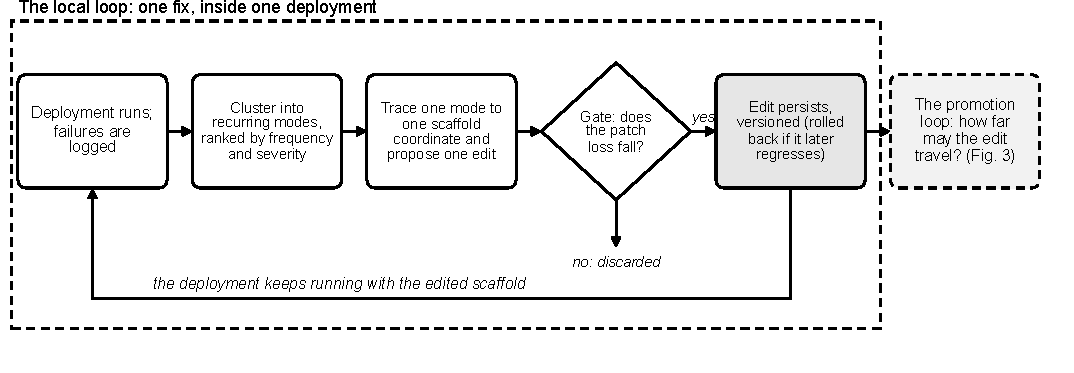
\includegraphics[width=\textwidth]{figures/fig1_descent}
\caption{Loop 1, the local half of artifact-layer descent. A recurring failure is traced to one scaffold coordinate, one edit is proposed, and a gate keeps the edit only if the deployment's patch loss falls. An accepted edit then enters Loop 2 (Fig.~\ref{fig:scope}).}
\label{fig:descent}
\end{figure*}

Loop 2 is the step most systems skip. An engineer notices that a coding agent keeps misnaming a class in one repository. The fix is a one-line rule in that repository's instruction file. That same rule could be promoted to a team-wide template, to the company's core instructions, or to a skill registry shared across companies. The edit did not change; its scope did. And the gate that should let it through gets stricter at each step, because the loss it is tested against is now an average over more deployments, and a fix that helps one repository can hurt another.

The scopes nest (Fig.~\ref{fig:scope}). USER is one person's account or fork; PROJECT is one repository, workflow, or product workspace; STACK is a curated bundle of projects under one team; a \textbf{tenant} is one organization or customer; CORE is the scope every tenant shares. Each level's loss is the average failure rate over the deployments it contains. Promotion that reaches CORE crosses tenants, which is what cross-tenant promotion means here. Loop 2 promotes an edit upward only as far as the evidence reaches; we call that limit the edit's \textbf{evidence radius}. The check that belongs at each rung is \textbf{receiving-side evaluation}: a check run where the edit arrives, not where it was made. In optimizer terms, Loop 1 sets the step (how much one accepted edit changes the local scaffold) and Loop 2 sets the target (which average failure rate the scaffold is tuned to reduce). Governance is therefore not administrative overhead. It is the regularization that keeps a small fix from being aimed at the wrong target.

\begin{figure}[htbp]
\centering
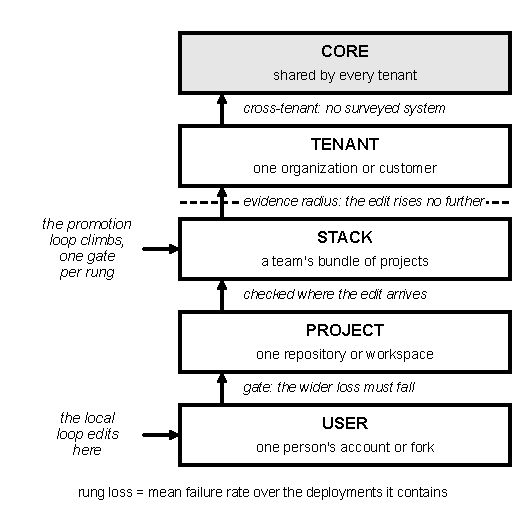
\includegraphics[width=0.55\textwidth]{figures/fig2_scope}
\caption{Loop 2, the promotion half. Scopes nest from USER to CORE, each rung's loss averages the deployments it contains, and an edit rises one rung at a time, only while a check at the receiving side shows the wider loss falling and only as far as its evidence radius. Promotion into CORE crosses tenants.}
\label{fig:scope}
\end{figure}

\subsection{When the loop is an optimizer}\label{when-the-loop-is-an-optimizer}

The loop is an optimization process, rather than a description of good practice, when five conditions hold:

\begin{enumerate}
\def\labelenumi{\arabic{enumi}.}
\tightlist
\item
  a measurable patch loss, such as a failure rate, a correction rate, or an evaluation score;
\item
  captured residuals, so that failures are logged rather than lost;
\item
  credit assignment, so that a failure can be traced, at least sometimes, to the scaffold coordinate that caused it;
\item
  a synthesized candidate edit to that coordinate; and
\item
  a gate that checks whether the edit lowers the loss before the edit is kept or promoted.
\end{enumerate}

The conditions presuppose frozen frontier weights, edits that persist as inspectable artifacts rather than transient prompts, and promotion that widens an artifact's scope under a gate rather than averaging comparable updates as weight-space federated learning does.

Written out, the patch loss of deployment \(D\) is \[L_D(\theta_s) = \mathbb{E}_{x \sim D}\!\left[\ell(\pi(\theta_M, \theta_s, x))\right],\] where \(\theta_M\) are the frontier weights, fixed during deployment, \(\theta_s\) is the scaffold, a structured object over the six substrate coordinates of Section~\ref{sec:method}, and \(\ell\) is an operational loss. A failure yields no analytic gradient. It yields a candidate edit \(z_t\), proposed by reflecting over the accumulated failure history. The gate accepts the edit when its noisy estimate of the change in loss clears a margin, \[G_t(z_t) = 1 \iff \widehat{\Delta}_{z_t} L_D(\theta_s^t) + \lambda\,\Omega(z_t) \le -\tau_t,\] where \(\Omega \ge 0\) penalizes the complexity of the edit and the breadth of its promotion, and \(\tau_t \ge 0\) is the required margin. Production systems implement this inequality without ever writing it down: an evaluation blocks a merge on regression, a reviewer rejects a vague rule, a governance system holds an artifact back until evidence accumulates. Under a bounded-bias assumption on the gate, the update satisfies a one-step descent inequality. When that bias is summable over the run, the loss converges and improving edits stop clearing the gate; the scaffold is then gate-stable, which is a statement about the gate, not about optimality (Appendix~\ref{app:formal}). Where a condition fails, the picture is an analogy, and the survey marks which systems meet which conditions.

Each half of the loop has a gate, and we name three kinds by who decides. A gate is \textbf{Auto} when a program applies a check before the edit goes through: an evaluation score, a verifier, a reinforcement-learning threshold, or a language-model judge \cite{zheng2023judge} with a quantified agreement rate. It is \textbf{Human} when a person decides. It is \textbf{None} when nothing decides, either because that half of the loop is absent or because the step runs unchecked, as when a system pushes every edit to its neighbors without a test. Who writes the candidate is recorded separately and is not a gate: the author may be an agent reflecting over failures, an engineer at a desk, or a contributor registering an artifact. We write a system's two gates as a pair, Loop 1 first: {[}Auto × Human{]} means an algorithmic local gate and a human promotion gate. These pairs index the design space of Section~\ref{sec:design}.

Condition 1 says the loss must be measurable. It does not say what measures it, and that turns out to be the question that sorts the corpus.

\subsection{From patchwork to descent}\label{from-patchwork-to-descent}

Three stages of scaffold maintenance recur across the corpus, and the five conditions separate them. Take the coding agent above that keeps misnaming a class. At the first stage, patchwork, an engineer adds a rule to the instruction file after noticing the failure; nobody measures whether it helped, nothing is promoted on evidence, and the file sprawls with every incident until nobody knows which rule does what. At the second stage, random artifact search, the system tries many variants of the file under the test suite and keeps the best. The suite is the only signal and no failure is traced to the rule that caused it; the winning variant has learned the suite as much as the task. At the third stage, artifact-layer descent, the recurring failure is traced to the one rule responsible, one edit is proposed, the gate checks that the patch loss falls, and promotion stops at the evidence radius and can be reversed. A loop reaches the third stage once the five conditions hold, and its dominant failure becomes evaluation fragility, because the suite that gates the edits is itself a scaffold artifact that drifts and can be gamed (Section~\ref{sec:failure}). Production deployments that reach it on Loop 1 then promote in one of two ways: behind a human gate, as Spotify \cite{palumbo2026spotify} and SkillForge do, or, in Letta's Context Repositories alone, by an ungated push that carries lineage but no evaluation.

Two consequences of condition 1 follow the loop everywhere, and the survey keeps returning to them. The first is that the measure bounds the lift. An accepted edit is an improvement in what the gate measured, on the tasks the gate sampled, and nothing more; a rule that lowers the failure rate on one repository's suite has earned nothing about another repository's. Every loss has a scope. That is why Loop 2 cannot carry Loop 1's evidence: the receiving scope measures a different mix of tasks, so a promoted edit either travels under a measure the scopes share or re-establishes its lift where it arrives, which is what receiving-side evaluation is for. Where tenants measure different things, a lift does not transfer at all without it.

The second is that the loop optimizes and does not evolve. It needs a defined measure before it can start and descends toward that measure's ceiling; at the ceiling no edit clears the gate, which is what gate stability means. It does not discover a better goal than the one its measure encodes. Two scaffolds optimized for the same goal under the same measure need not converge to one version; each stops at the ceiling by its own route. A system that edits its own measure, the reflexive gate of Section~\ref{sec:signal}, moves the destination rather than evolving toward an unknown truth. The distinction matters because the corpus is often described in the vocabulary of evolution; what the gated systems in it actually do is descent.

\section{Where the signal comes from: four classes of feedback}\label{sec:signal}

Four scaffolds all run the loop of Section~\ref{sec:loop}. A coding agent changes one line in its repository rule file; the test suite runs and reports pass or fail within seconds. A scheduling assistant changes how it phrases a booking request; the appointment either appears on the calendar or it does not, and the system learns which an hour later. A marketing assistant changes the tone rule in its instructions; nobody can say whether the next draft is better, only whether a reviewer prefers it. A research assistant changes how it chooses which direction to pursue; whether the choice was good becomes visible months later, after many other edits have landed. All four produce a candidate edit. They differ in what the gate can know about it.

That difference is the whole of this section. The gate needs an estimate of one quantity: whether the edit lowered the patch loss. That estimate comes from a feedback signal. Signals differ in three ways: how soon they arrive, how exact they are, and whether there is a fact of the matter at all. Those three differences sort every surveyed system into four classes (Table~\ref{tab:IV-1}), and the class fixes what the gate can be, which half of the loop can close automatically, and which failure dominates.

\begin{table}[htbp]
\caption{The four feedback-signal classes. Reading across a row: what the gate receives, what it can therefore be, and what it cannot fix.}\label{tab:IV-1}
\centering\small
\begin{tabular}{@{}
  >{\raggedright\arraybackslash}p{(\linewidth - 8\tabcolsep) * \real{0.1011}}
  >{\raggedright\arraybackslash}p{(\linewidth - 8\tabcolsep) * \real{0.2697}}
  >{\raggedright\arraybackslash}p{(\linewidth - 8\tabcolsep) * \real{0.2247}}
  >{\raggedright\arraybackslash}p{(\linewidth - 8\tabcolsep) * \real{0.2472}}
  >{\raggedright\arraybackslash}p{(\linewidth - 8\tabcolsep) * \real{0.1573}}@{}}
\toprule\noalign{}
\begin{minipage}[b]{\linewidth}\raggedright
Class
\end{minipage} & \begin{minipage}[b]{\linewidth}\raggedright
The signal the gate receives
\end{minipage} & \begin{minipage}[b]{\linewidth}\raggedright
What the gate can be
\end{minipage} & \begin{minipage}[b]{\linewidth}\raggedright
What stays hard
\end{minipage} & \begin{minipage}[b]{\linewidth}\raggedright
Corpus examples
\end{minipage} \\
\midrule\noalign{}


C1 exact & A check that returns pass or fail, or an exact score, at once and repeatably: tests, compilers, answer keys & An automatic check; one run per case, repeated only to sample the task mix & The lift is bounded and specific, an improvement in what the check measures on the cases it ran; the check names the failed output, not the coordinate that caused it; a check that is also the target can be gamed & DGM, AlphaEvolve, SkillOpt \\ \addlinespace[2.5pt]
C2 observable outcome & A real result one episode later: a booked slot, a merged pull request, a closed ticket; noisy and confounded & An automatic threshold over batched episodes; a person at promotion & The outcome says \emph{that} the episode failed, not \emph{why}; the channel can be poisoned & Devin, Sierra, SAGE, SkillRL, PACE, Voyager \\ \addlinespace[2.5pt]
C3 judged & A rater, a rubric, or a model judge; no ground truth & A judge calibrated against people; a person at promotion & The rubric is itself a scaffold coordinate, so the gate judges edits to itself; the proxy gets optimized past the point where it tracks quality & SkillForge, CASCADE, skills-repository review \\ \addlinespace[2.5pt]
C4 delayed & An outcome weeks or months later, once per many edits & No per-edit gate; proposals are pruned and milestones stand in & Credit across many edits; drift; the loop cannot be told from random search & NanoResearch, CORAL, the AI Scientist \\ \addlinespace[2.5pt]
\bottomrule\noalign{}
\end{tabular}
\end{table}

The classes are a partition, not three independent axes: a system is assigned by the property that binds its gate first. Delay binds before anything else, so an outcome that arrives months later is C4 even when it is objective; the absence of ground truth binds next, so an immediate judgment is C3; and among signals that are prompt and objective, exactness separates C1 from C2.

\textbf{C1, exact.} A deterministic checker returns pass or fail, or an exact score, immediately and repeatably: unit tests, compilers, type checkers, exact-match answer keys, proof checkers, schema validators. DGM accepts a self-modification only after it passes in a sandbox on coding benchmarks \cite{zhang2025darwin}; AlphaEvolve scores candidate programs with a cascade of exact evaluators \cite{alphaevolve2025}; SkillOpt gates a skill edit on a held-out exact-match split of a math benchmark \cite{yang2026skillopt}. Because the check is exact for the artifact and the test it runs, and repeating it returns the same answer, one run settles the checked case. What the check does not settle is the patch loss: the suite is a sample of the patch's task mix, and the agent that runs under the edited scaffold is stochastic, so the gate's estimate of the loss change still carries sampling error. The gate can be a program and its margin can be small, but the margin absorbs sampling error, not error in the check. The improvement the check certifies is also bounded and specific: an improvement in what the check measures, on the cases it ran, not an improvement in general. Two things stay hard. A failing test localizes the output, not the scaffold coordinate that caused it, so credit assignment remains open; and a checker that is also the training target can be gamed. The dominant failures are test overfitting and scaffold bloat, because cheap acceptances accumulate.

\textbf{C2, observable outcome.} The environment or the user emits an outcome after an episode: a booked appointment, a closed ticket, a merged pull request, a tool call that returns without error, a retrieved document that contains the answer. The signal is real but one episode late, noisy, and confounded, since a user can accept a wrong answer and reject a right one. Gates of this class include Devin's merged pull requests \cite{cognition2025devinreview}, SAGE's task success on AppWorld \cite{wang2025sage}, SkillRL's success-rate threshold \cite{skillrl2026}, and PACE's failure signals from a deployed small model \cite{ling2026pace}. The gate can still be a program (a reinforcement-learning threshold or a held-out task suite), but it needs a positive margin, and it absorbs the noise by batching episodes or by requiring agreement across samples (Appendix~\ref{app:gates}). Credit assignment takes its most stubborn form here: the outcome says \emph{that} the episode failed, not \emph{why}. Most production deployments live in this class, and its signal arrives through a channel an attacker can control, which is why poisoned memory and tool-output injection dominate.

\textbf{C3, judged.} There is no fact of the matter. An essay, a marketing page, a design, a pitch deck, or a code review for style can be scored only by a judge: a human rater, a language-model judge, a rubric, or a comparison against references. SkillForge accepts a skill diff when its judge agrees with human engineers more than nine times in ten \cite{skillforge2026}; CASCADE consolidates memory under a human-and-agent gate \cite{huang2025cascade}; Anthropic's skills repository promotes a skill when a reviewer approves the pull request. The gate can be a program only after the judge has been calibrated against people, because the judge's bias is now the estimator's bias. Residuals, meanwhile, are captured only when someone objects, so condition 2 depends on complaint channels rather than instrumentation. The dominant failure is Goodhart's law in the form measured for reward models: optimizing a proxy past a point lowers the true score \cite{gao2023overoptimization}. Once the judge is the target, the scaffold learns the judge. Nor is a human judge stable: Shankar et al.~find that evaluators' criteria drift as they grade more outputs \cite{shankar2024validators}.

\textbf{C4, delayed and sparse.} The outcome arrives after weeks or months, once per many edits, in a world that has moved on. Research programs, product strategy, and open-ended discovery are of this kind; the clearest instances are automated research pipelines such as the AI Scientist, which generates ideas, runs experiments, and writes the paper \cite{lu2024aiscientist}. NanoResearch merges candidate skills by semantic compatibility rather than by a measured loss change \cite{xu2026nanoresearch}, and CORAL promotes findings into shared memory on a heartbeat rather than on an evaluation \cite{qu2026coral}. AlphaEvolve's evolutionary database can look like an instance, and is not one: it balances improving the best programs against diversity only after every candidate has been scored by its exact evaluators, so it is a search strategy inside the exact class, not a gate for a delayed signal \cite{alphaevolve2025}. With no per-edit estimate to gate on, the gate degenerates to proposal pruning plus proxy milestones, and the descent argument covers only the composition of pruning and whatever gate exists at the horizon (Appendix~\ref{app:gates}). Temporal credit assignment across many edits is open. The dominant failure is drift: the scaffold ages faster than the signal that would correct it. An optimizer in this class also cannot be told from random search by its outcomes alone; Ong et al. \cite{ong2026harnesseval} report the same indistinguishability for harness optimizers.

\textbf{The judge is part of the scaffold.} The judged class has one feature the other three lack: the rubric that sets the loss is itself a scaffold coordinate, and it returns in the findings and in the open problems. Suppose a pitch-review system keeps overrating decks that claim a large market without numbers. It traces the failure to its rubric and edits ``evaluate market size'' into ``require a numeric estimate and a source''. That edit changes the gate that will judge the next edit. We call this the \emph{reflexive gate}, and nothing in the corpus calibrates one: three scaffold systems report judge calibration \cite{skillforge2026, hu2026skillchain, zhu2026skillcoach}, and none calibrates a judge that is itself being edited. The weight side faces the same question. Reinforcement learning from verifiable rewards lies outside the scored corpus, but pushing it into writing and other open-ended tasks has forced researchers to build judged gates. One group holds the gate fixed while the policy learns, as a checklist, a pairwise judge, a reference-anchored judge, or a fixed rubric \cite{gunjal2025rubrics, jia2025writingzero, shi2026references, jin2026rlaes}; a second group lets the gate move with the policy, scoring by the policy's own probability of a reference or updating the rubric or judge during training \cite{yu2025rlpr, xu2026rubricarm, ding2026evorubrics, zhu2026score, li2026rubricem}. Fixed versus co-evolved is exactly the reflexive-gate question, and of the co-evolving methods only RLPR, whose reward is a probability rather than a rubric, reports agreement with human labels (Appendix~\ref{app:audit}).

\textbf{What the class decides.} Read down the table and three consequences follow, each a prediction about the corpus that Section~\ref{sec:design} checks. First, which half of the loop can close automatically. An exact check or an observed outcome can gate a local edit by program. A judgment can do so only once the judge is calibrated, and a delayed reward cannot gate edits one at a time. Promotion is stricter. Only the exact class carries its own measure to the receiver, and only when the receiving side runs the same check: that is the one case in which the sending side's evidence means the same thing on arrival. In every other case the receiving-side evaluation of Section~\ref{sec:loop} is still owed. Second, which gate pairings a deployment can reach. {[}Auto × Auto{]} belongs to exact signals and simulated outcomes; {[}Auto × Human{]} belongs to observed outcomes and judgments, where the person on Loop 2 does the work the missing exact signal cannot; and the delayed class has no per-edit gate on either half. Third, which failure dominates, as the last column of the table records and Section~\ref{sec:failure} develops.

\section{The corpus, and how it was read against the loop}\label{sec:method}

Every placement in Sections~\ref{sec:findings} to \ref{sec:failure} is a reading of one system's own text in the vocabulary of Section~\ref{sec:loop}: which scaffold coordinate the system edits, whether a measure gates the edit, who decides, and how far the edit travels. The reading was done from each system's method section or documentation, and it is released row by row with a one-line justification, so that any placement below can be checked against the system rather than against this survey.

\subsection{How the corpus was assembled}\label{how-the-corpus-was-assembled}

A system enters the corpus if it wraps a foundation model with at least one persistent artifact updated from deployment signal, or if it is described in public as self-improving, scaffolded, or agentic; systems whose only update mechanism is weight-level training, and systems with no public evidence of deployment or release, are excluded (Appendix~\ref{app:data}). The systems were found in public sources in two passes (130 by May 2026 and 126 more by the October 2026 cutoff), and the second pass records, for each system it added, the gate on each half of the loop, the signal class, and the governance properties as columns of the released table, so the counts that follow by gate and by class are counts over the systems it added.

Two filters sort the systems (Fig.~\ref{fig:corpus}), and both are stricter than the field's own labels. The first keeps a system in the core corpus only when some artifact of it persists across scope or is updated from feedback, which is a score of at least 3 on at least one substrate on the ruler below; systems that carry the labels but fail it form a contrast corpus, kept so that the boundary can be audited rather than asserted. Of the 256 systems, 204 form the core corpus and 52 the contrast corpus. Every system is scored on each substrate it adapts, and a system that adapts several gets one composite row as well, which is why 256 systems give 269 rows.

\begin{figure}[htbp]
\centering
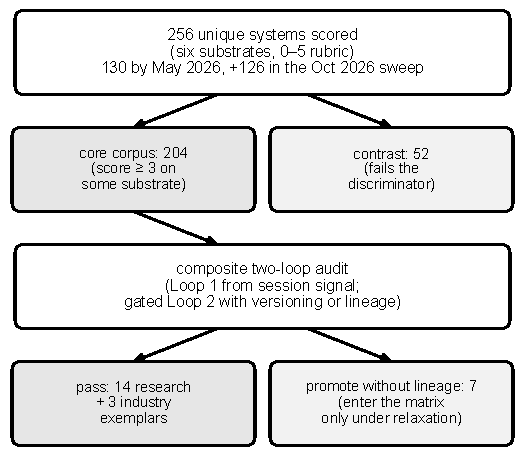
\includegraphics[width=0.55\textwidth]{figures/fig4_corpus_flow}
\caption{Corpus flow. Every system is scored on the substrates it adapts, with an integrated row for systems that adapt several, giving 269 substrate-level rows for 256 systems; the discriminator splits core from contrast; the composite two-loop audit selects the systems placed in the design space of Section~\ref{sec:design}.}
\label{fig:corpus}
\end{figure}

The second filter is the two-loop audit, which asks each core system the two questions of the loop's two halves: does Loop 1 modify a persisted artifact from session signal, and does Loop 2 promote the artifact beyond the deployment that produced it, with versioning or lineage? Applied to the 204 core systems, and to ten more classified from their papers alone (they are not rows of the released table), it admits 14 research systems (13 table rows and SkillOpt) and 3 industry exemplars (Sierra Agent OS 2.0, Cognition Devin, and Letta's Context Repositories). These are the systems the gate grid of Section~\ref{sec:design} places by who decides on each half; the grid's lighter cells also show curation and, for comparison, the systems with no failure-driven loop, and the systems that promote without lineage join cells already occupied. Passing the audit is a weaker thing than having the governed second loop of the thesis: every passing system promotes across users, teams, or repositories inside one operator, none reaches another organization, and one of them, Letta, promotes with no gate at all (Section~\ref{sec:gap}).

\subsection{Six coordinates and one ruler}\label{six-coordinates-and-one-ruler}

Condition 3 of Section~\ref{sec:loop} asks that a failure be traced to the scaffold coordinate that caused it, and the corpus locates that coordinate on one of six substrates (Table~\ref{tab:V-1}); they are the coordinates of \(\theta_s\), each editable independently of the others, and the three kinds of memory on the memory substrate follow the cognitive-architecture taxonomy of Sumers et al. \cite{sumers2023coala}.

\begin{table}[htbp]
\caption{The six scaffold substrates, what each holds, and what a system must do on it to score 5.}\label{tab:V-1}
\centering\small
\begin{tabular}{@{}
  >{\raggedright\arraybackslash}p{(\linewidth - 4\tabcolsep) * \real{0.1642}}
  >{\raggedright\arraybackslash}p{(\linewidth - 4\tabcolsep) * \real{0.4179}}
  >{\raggedright\arraybackslash}p{(\linewidth - 4\tabcolsep) * \real{0.4179}}@{}}
\toprule\noalign{}
\begin{minipage}[b]{\linewidth}\raggedright
Substrate
\end{minipage} & \begin{minipage}[b]{\linewidth}\raggedright
What persists
\end{minipage} & \begin{minipage}[b]{\linewidth}\raggedright
A score of 5 requires
\end{minipage} \\
\midrule\noalign{}


S1 Instructions & Project, team, or organization rules attached to a workspace & Versioned rules promoted under an automatic gate \\ \addlinespace[2.5pt]
S2 Skills & Procedures, as code or text, loaded on demand & A skill bank that edits itself on failure, test-gated, versioned, and promoted \\ \addlinespace[2.5pt]
S3 Memory & Experience kept across sessions: episodic, semantic, procedural & Provenance, versions, and a correction path for every entry \\ \addlinespace[2.5pt]
S4 Tools & The vetted action surface and its schemas & Evaluation-gated tool versions; a curated bundle as the product \\ \addlinespace[2.5pt]
S5 Orchestration & The multi-role graph and its routing & Topology updated from an outer-loop signal \\ \addlinespace[2.5pt]
S6 Governance & Versioning, promotion, audit, rollback & Staged promotion with evaluation thresholds, an audit log, and rollback \\ \addlinespace[2.5pt]
\bottomrule\noalign{}
\end{tabular}
\end{table}

The ruler is the same on every substrate, 0 to 5, and it measures distance along the loop. At 0 the artifact is ephemeral; at 1 it is persistent and local; at 2 it is persistent with tool attachment but no feedback; up to that point an artifact persists and nothing measures it, which is the patchwork stage of Section~\ref{sec:loop}. At 3 the artifact either spans scopes with no gate on the way or is updated from feedback by a person; at 4 a program updates it from feedback, so Loop 1 closes. The top mark, 5, is each substrate's own in Table~\ref{tab:V-1}: both halves of the loop on the substrates that hold adaptable content (S1, S2, S5), and the machinery a second loop would need on those that hold governance (S3, S4, S6), which is why a registry or a prompt platform can score 5 with no Loop 1 at all.

\subsection{What was gathered, by substrate}\label{what-was-gathered-by-substrate}

No system matures all six substrates at once (Table~\ref{tab:V-2}). Research systems learn fast and lack enterprise governance; production systems govern well and learn slowly; open standards solve artifact portability but not adaptation. Each kind was built to satisfy one constraint (fast learning, safe change, or portability) and matured only the substrates that constraint touches, so the top marks fall on different substrates for different kinds of system: research systems on skills and memory and in the composite row, products and standards on tools and governance, and no system at all on instructions or orchestration.

\begin{table}[htbp]
\caption{Substrate maturity across the 256-system corpus. Column n counts scored rows on each substrate, Mean is the average score, and Score-5 systems reach the substrate's top mark; the composite row counts systems scored across several substrates as one row. Of the 126 most recently added systems, 102 are core and 31 are skill systems; 92 of those core systems close Loop 1 under a program, and none of the 126 scores 5 on any substrate.}\label{tab:V-2}
\centering\small
\begin{tabular}{@{}
  >{\raggedright\arraybackslash}p{(\linewidth - 8\tabcolsep) * \real{0.1600}}
  >{\raggedleft\arraybackslash}p{(\linewidth - 8\tabcolsep) * \real{0.0533}}
  >{\raggedleft\arraybackslash}p{(\linewidth - 8\tabcolsep) * \real{0.0667}}
  >{\raggedright\arraybackslash}p{(\linewidth - 8\tabcolsep) * \real{0.2667}}
  >{\raggedright\arraybackslash}p{(\linewidth - 8\tabcolsep) * \real{0.4533}}@{}}
\toprule\noalign{}
\begin{minipage}[b]{\linewidth}\raggedright
Substrate
\end{minipage} & \begin{minipage}[b]{\linewidth}\raggedleft
\(n\)
\end{minipage} & \begin{minipage}[b]{\linewidth}\raggedleft
Mean
\end{minipage} & \begin{minipage}[b]{\linewidth}\raggedright
Score-5 systems
\end{minipage} & \begin{minipage}[b]{\linewidth}\raggedright
What the corpus holds on it
\end{minipage} \\
\midrule\noalign{}


S1 Instructions & 15 & 3.07 & (none) & Rules persist across IDEs and agents and nothing measures them; no system closes both loops; ceiling 4 \\ \addlinespace[2.5pt]
S2 Skills & 50 & 3.34 & SAGE, COSPLAY & Loop 1 closes under a program in the research systems; the production repositories merge by hand \\ \addlinespace[2.5pt]
S3 Memory & 50 & 3.06 & Cuadros et al. & The ledger ships in products; the correction a gate would enforce is absent \\ \addlinespace[2.5pt]
S4 Tools & 20 & 3.65 & MCP, Harvey, Hippocratic AI & The most mature production substrate; registries govern admission, not evaluation \\ \addlinespace[2.5pt]
S5 Orchestration & 37 & 3.08 & (none) & Topologies change under an evaluation gate; one structurally gated instance; no two-loop system \\ \addlinespace[2.5pt]
S6 Governance & 45 & 3.02 & Braintrust, Vellum, LangSmith Hub, AGENTS.md/AAIF & Prompts-as-code mature; registries add lineage and rollback; no Loop 1 generates a candidate \\ \addlinespace[2.5pt]
Integrated & 52 & 3.81 & NanoResearch, AutoAgent, SkillRL & High-water mark; reached only by research systems without enterprise governance \\ \addlinespace[2.5pt]
\bottomrule\noalign{}
\end{tabular}
\end{table}

\subsection{Evidence and scoring discipline}\label{evidence-and-scoring-discipline}

Every classification rests on public evidence of uneven strength and on one rater. Each system carries one or more evidence tiers (T1 to T5 in the released table: peer-reviewed publication, arXiv preprint, production claim with metrics, open-source artifact, industry blog or interview); peer-reviewed papers and open-source artifacts weigh most in corpus-level statements, a production claim counts when it names a benchmark or integration target, a blog post or interview counts only when a higher tier corroborates it, and production claims are never pooled with peer-reviewed evidence in a corpus-level statistic. Industry systems evaluated from vendor documentation rather than a paper are flagged wherever they appear. One author scored every system, used half-scores only when one criterion was clearly met and another partially, and rounded ambiguous cases down; the scores have not been independently re-rated, and that check is future work. The complete score table, with a one-line justification per row, is released so that every scored classification can be re-derived (Appendix~\ref{app:scores}); the counts move under natural relaxations of the audit (counting rollback alone as Loop-2 governance, asking for a promotion mechanism with no governance at all, admitting a Loop 1 that persists only optimizer state) while the qualitative findings survive every one of them (Appendix~\ref{app:data}).

\section{Loop 1 in the industry: a failure, one edit, a gate}\label{sec:findings}

The local half of the loop is built, and it is built from the gate backward. In nine of ten of the most recently added core systems a program keeps or discards each local edit on a measured loss, and the pattern holds on every substrate that has a failure-driven loop at all (Table~\ref{tab:V-2}). What stands before the gate is far less built: production deployments log preferences and successes rather than failures, so there is little to cluster, and no general method traces a failed output to the coordinate that caused it. What stands after the gate is half built: the memory products keep every entry's history and still return facts that were revoked. Walked in the order it runs, from the logged failure to the kept edit, Loop 1 is a gate the field has made well, fed by a trace it has hardly made at all.

\subsection{The failure and its trace}\label{the-failure-and-its-trace}

Condition 2 asks that failures be logged rather than lost, and in production they are mostly lost. Deployed memory systems record preferences and successful facts, not residuals, so the loop has little to cluster. The one field report of a store that records dead ends so they are not repeated describes a single, self-reported deployment \cite{helwig2026memory}; everywhere else the log that Loop 1 would cluster is never written. The gap sits in the observable-outcome class (C2), where an episode is recorded as a success or a preference and the failure that would have been the residual leaves no entry.

Which sessions inform the next edit is left to chance. The loop of Section~\ref{sec:loop} ranks recurring modes by how often they recur and how badly they fail before it takes one up; nearly every system in the corpus takes failures in the order they arrive instead. Task-CoEvolve's variance-weighted task sampling and AutoSaddler's mini-batch failure signals are the exceptions \cite{miyai2026taskcoevolve, park2026autosaddler}, and both weight the sessions the loop learns from by how much they disagree (C2). A loop that learns from whatever arrived last is descending on a sample nobody chose.

Condition 3, tracing a failure to the coordinate that caused it, is the step the field itself names as the bottleneck: the harness-optimization line and the evaluation of harness optimizers by Ong et al.~agree that attributing a system-level failure to one scaffold coordinate is what separates descent from trial and error \cite{lin2026ahe, zehle2026cantante, lee2026metaharness, nguyen2026harnessevo, liu2026skillsvote, ong2026harnesseval}. Where it is solved, it is solved one substrate at a time. Meta-Harness keeps a filesystem of candidate harnesses that records which edit helped, and that record is the history the loop reflects over \cite{lee2026metaharness}; SkillsVote attributes each outcome to skill, exploration, or environment before an update is admitted \cite{liu2026skillsvote}; SkillOpt-Lite's consensus filter across rollouts is the form of credit assignment its ablation finds load-bearing \cite{shen2026skilloptlite}. In the general case, where a failed output may come from a stale memory entry, an under-specified rule, or a misrouted edge, the trace remains unsolved. A gate can keep only the edit it is given, and the step that would say which coordinate to edit is the one the field has hardly built.

\subsection{The edit and the pool}\label{the-edit-and-the-pool}

Three kinds of author write the candidate of condition 4, and who writes it decides how often the loop can start. In the research systems an agent writes it by reflecting over the failure history, which is the author the loop of Section~\ref{sec:loop} assumes. In the prompts-as-code platforms an engineer writes it at a desk, and session feedback never triggers a candidate (Section~\ref{sec:design}). A contributor writes it in the public skill repositories, where every substantive edit is human-authored and human-merged \cite{shen2026whomaintains}. Who writes the candidate is not a gate, but where the author is a person Loop 1 runs only as often as a person notices.

The pool the candidate enters is governed as carefully as the candidate. Eleven skill systems treat removing an artifact as an operation that must pass a check, the same as adding one \cite{zhang2026librarydrift, wei2026skillsmith, pu2026skillops, wang2026assay}. The reason is in Ratchet's result: skills written by a language model gain nothing over a no-skill baseline until lifecycle hygiene is applied, while human-curated ones show a double-digit gain \cite{zhang2026ratchet}. A pool nobody prunes starves the gate of signal, because failures caused by stale artifacts cannot be told from failures the edit under test would fix (Section~\ref{sec:failure}). Hygiene is not an alternative to descent; it is what makes the gate readable.

\subsection{The gate: what it measures, who decides, how long it waits}\label{the-gate-what-it-measures-who-decides-how-long-it-waits}

Wherever a failure-driven loop runs on skills or orchestration, the local gate is now a program, with one exception, and the research activity is concentrated there. On skills, SAGE and COSPLAY close both halves of the loop inside one research environment \cite{wang2025sage, wu2026cosplay}; the exception is SkillChain, which puts a person after the judge, a human reflection gate before an edit reaches the skill bank \cite{hu2026skillchain}. On orchestration, topology changes are evaluation-gated and no system closes both loops: GPTSwarm's optimizable graphs \cite{zhuge2024gptswarm} and AFlow's tree search over code-represented workflows \cite{zhang2024aflow} searched for a topology under a score; Optimas, AgentGrad, and HarnessForge keep a change only under an evaluation \cite{cheng2026optimas, chu2026agentgrad, chen2026harnessforge}, and TOCOMAS keeps it only when it also satisfies a structural invariant \cite{zhao2026tocomas}.

The counter-example is the most widespread artifact of all. Instruction files persist across IDEs and agents (Claude Code, Cursor, AGENTS.md \cite{agentsmd2025}, Windsurf, Continue.dev) and appear in a fifth to a quarter of coding-agent projects \cite{robbes2026agenticmuch, galster2026harnessconfig}, yet in the one controlled study they raise inference cost by about a fifth and buy nothing in task success \cite{gloaguen2026agentsmd}. That is the patchwork stage of Section~\ref{sec:loop} on the most widely deployed substrate: a rule is added after a failure, nothing measures whether it helped, and the file grows. A rule file that nobody measures is patchwork at scale.

Read by who decides, the three gate kinds of Section~\ref{sec:loop} fall on Loop 1 in a fixed pattern. A program decides nearly everywhere a failure-driven loop runs. A person decides only in curation, where an agent drafts and a person chooses what is kept, as in VerificAgent's fact-checked and frozen memories \cite{nguyen2025verificagent} and SkillChain's final reflection gate. Where no local loop exists, in the prompts-as-code platforms and the registries of Section~\ref{sec:design}, nothing decides on Loop 1 at all; what those systems gate is admission to a shared pool, which is a Loop 2 decision. The pattern is the one Section~\ref{sec:signal} predicts for the local half: a program wherever the loop has a check or an outcome to read, or a judge calibrated against people.

How long the gate waits is where the newer systems differ from the earlier ones. The earlier systems accepted an edit on one evaluation and absorbed the estimator's noise through the margin alone; the newer ones wait. SAGE-gate commits an edit only when a paired per-item test says its wins are reliable \cite{wang2026sagegate}; in VaG, three heterogeneous critics must pass \cite{shang2026vag}; AutoSaddler feeds mini-batch failure signals into validation-based selection \cite{park2026autosaddler}. Waiting hides two different operations: if each of \(k\) independent proposals is wrongly accepted with probability \(p\), requiring all \(k\) to agree drives the false-accept rate to \(p^k\), while averaging \(k\) noisy scores shrinks the variance of the estimate only by \(1/k\) (Appendix~\ref{app:gates}). A gate that waits for a batch is condition 5 taking the noise in condition 1 seriously, and in the corpus that care arrived after the gate itself.

\subsection{The ledger: versioned, not corrected}\label{the-ledger-versioned-not-corrected}

Versioning and rollback are the last step of Loop 1: an accepted edit stays in the scaffold and is reversed if a later check shows it made things worse. They are also the record a second loop would read, and the memory products have built the record and not the correction. Letta's git-backed Context Repositories \cite{letta2026memfs}, Mem0's per-memory history \cite{mem02026history}, and Zep's bitemporal facts \cite{zep2026facts} all record how an entry came to be, so a user who asks what the system remembers and why can be answered. Research memory splits into write-gating and provenance on one side \cite{wang2026toki, xu2026ppmf, margalit2026governed} and verifier-gated failure loops on the other \cite{yu2026recuris, wang2026memguard, sun2026vermem}, and only the governed collaborative memory of Cuadros et al.~does both \cite{cuadros2026governed}, which is why it alone reaches the top mark.

What lineage does not give is correction. Five production backends still return facts that were revoked \cite{shen2026revoked}: the ledger exists, the gate that would act on it does not, and the gap sits in the observable-outcome and judged classes (C2, C3), where a revocation arrives as a user's objection rather than as a failed check. Rollback of a single edit inside one deployment exists, as edit-level reversal \cite{wei2026skillsmith, gao2026skillaudit} and as an admission test that rejects edits which cannot be undone \cite{sah2026evoundo}, and the one negative result on it cuts deep: once a contaminated skill has descendants, rolling it back recovers little, so gating must happen before commit \cite{shang2026vag}. No system rolls back a promotion that has crossed an organization, because none makes one (Section~\ref{sec:gap}). A memory that remembers its own history and cannot forget on request has the record a second loop would read, without the gate that would act on it.

\section{Loop 2 in the industry: how far an edit travels, and who lets it}\label{sec:design}

The second half of the loop exists in parts, and the parts sort by what they cross. Below the tenant boundary every kind of crossing is occupied inside one operator, from one user to another and one repository to another up to teams, and across the clients of a federated run. Who lets an edit climb is set by the feedback the crossing can get, as Section~\ref{sec:signal} predicted: a program where a check travels with the edit, a person where the signal is an observed outcome or a judgment, and in one production system nothing at all. Above the tenant boundary the scope exists and the promotion does not: CORE is settled across vendors as a format and a protocol, and what fills it is admitted by hand. On the gate grid the industry has converged on the local gate and is sorted on the promotion gate by its signal, and no system carries a promotion out of its operator under lineage, access control, and rollback.

\subsection{Inside one operator: what crosses, and the check where it arrives}\label{inside-one-operator-what-crosses-and-the-check-where-it-arrives}

Each crossing below the tenant boundary is occupied by a system of one operator, and a promotion differs from a push in having a check at all; the check that counts is the one where the edit arrives. The crossings run up the ladder of Section~\ref{sec:loop}. Between users, ShareMem consolidates one user's memories for another and evaluates them there \cite{hu2026sharemem}. Between repositories, a rule in XRepoSkill survives only if it is verified in at least two of them \cite{guo2026xreposkill}. Evo2Team promotes routing skills between teams (the STACK rung) and confirms them at the target \cite{wang2026evo2team}. Across the data-local clients of a federated run (partitions, not deployments of a tenant, so they sit on no rung), EvolveNet evolves a shared harness and accepts a merge only when it fixes at least as many held-out items as it breaks \cite{nie2026evolvenet}, and FederatedSkill's server agent applies, adapts, or rejects each client's patch and logs the decision \cite{yang2026federatedskill}. VACE checks a candidate against the model that will receive it, held fixed, before accepting it \cite{qi2026vace}; RASO adapts skills retrieved from a public corpus, which is inbound retrieval rather than promotion \cite{chu2026raso}.

Where the check sits is the next difference. ShareMem, XRepoSkill, Evo2Team, and VACE check where the edit arrives; EvolveNet checks at the aggregator and nowhere else; FederatedSkill records a decision taken at the server. The receiving-side evaluation that Section~\ref{sec:loop} places at every rung is therefore present in the corpus and rare, and where it is present it is necessary rather than sufficient: nearly a fifth of Evo2Team's confirmed transfers still fail on graphs the confirmation never saw.

None of these leaves its operator: no system promotes across customers or organizations with evidence. That is the thesis of this article, and because the failure log and the trace of Section~\ref{sec:findings} are hardly built, a system that tried would have little to promote and no way to check what it promoted.

\subsection{Who lets it climb: a program, a person, or nothing}\label{who-lets-it-climb-a-program-a-person-or-nothing}

A program lets an edit climb where a check travels with it. In AlphaEvolve, and in FunSearch before it, the evaluator cascade that scores every candidate is also the only thing that admits a program to the archive every later generation draws from, and the programs admitted that way went on to production gains at Google \cite{alphaevolve2025, romeraparedes2024funsearch}. It is a research loop run in production rather than a product, so it does not count against the two production routes of Section~\ref{sec:loop}, behind a person or not at all.

A person lets an edit climb where the signal is an observed outcome or a judgment. SkillForge shows the pairing most plainly: a judge that agrees with people more than nine times in ten passes each skill diff, and support engineers decide whether it ships \cite{skillforge2026}; CASCADE consolidates memory under a human-and-agent gate \cite{huang2025cascade}. Sierra routes agent-generated insights through human-authored expert answers \cite{sierra2025os20}. In Devin one event serves both halves: the merge of a pull request is the outcome Loop 1 reads, and the reviewer's decision to merge is also what lets the edit stand in the repository every later session uses \cite{cognition2025devinreview}. Spotify's automatically optimized prompts and plans go live only after an online A/B test and a launch decision \cite{palumbo2026spotify}. In every one of them the person on Loop 2 stands in for the exact signal production lacks, which makes the pairing the production-viable one rather than a compromise.

Nothing lets an edit climb in one production system. Letta's Context Repositories push every edit to shared memory with lineage and no check; the ledger records what crossed, and nothing asks whether it should have.

\subsection{The top rung: CORE exists, and everything in it is admitted by hand}\label{the-top-rung-core-exists-and-everything-in-it-is-admitted-by-hand}

CORE, the scope every tenant shares, exists today in two forms, and an edit promoted into it on evidence is not one of them. The first form is a format: Claude Agent Skills, Cursor Rules, GitHub Copilot instructions, Windsurf, Continue.dev, Zed, and Replit all keep a git-tracked markdown artifact attached to a workspace, with an MCP-style tool layer beside it \cite{galster2026harnessconfig, barbaste2026harnessengineering}, so an artifact written for one deployment can be carried to any other. The second form is a registry that admits artifacts for everyone, and admission is by hand: in the five public skill repositories of one field study, every substantive edit is written and merged by a person, with one deprecation in 254 edits \cite{shen2026whomaintains}; the MCP registries split into catalogues (namespaces and version records, no scanning) and control planes (scanning, access control, quarantine) \cite{agenticcommunity2026mcpgateway, microsoft2026apicentermcp, truefoundry2026mcpgateway}; and the governance registries bring lineage and rollback \cite{kang2026registry, quessadavial2026acm, qin2026governed}, none with evaluation-gated promotion. The prompts-as-code platforms hold the rest of the machinery a second loop would need, and nothing feeds it: Braintrust, Vellum, and LangSmith Hub \cite{braintrust2026docs, vellum2026docs, langsmith2026hub} keep immutable versions, evaluation thresholds, and rollback. But engineers author the candidates at a desk, an evaluation blocks a release on regression, and session feedback never triggers either, which makes them MLOps for scaffolds rather than for weights. Even where a repository runs an autonomous loop, the runtime state of that loop sits outside version control \cite{lulla2026loopengineering}, so what the format versions is the artifact and not the process that edits it. Registries govern what may be used and the platforms gate releases on evaluation, but neither generates a candidate from a failure, which is how tools and governance reach the top mark of Section~\ref{sec:method} with no Loop 1 at all.

\subsection{The two halves together: the gate grid}\label{the-two-halves-together-the-gate-grid}

\begin{figure}[htbp]
\centering
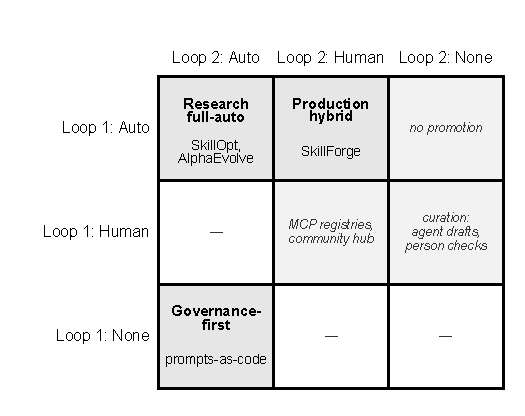
\includegraphics[width=0.5\textwidth]{figures/fig3_design_space}
\caption{The two-loop design space. Rows give the Loop 1 gate and columns the Loop 2 gate, with None for a step that is absent or runs unchecked; a cell [Loop 1 $\times$ Loop 2] such as [Auto $\times$ Human] pairs an algorithmic local gate with a human promotion gate. Darker cells mark the three populated kinds of system; lighter cells hold curation, the registries, and the systems whose promotion is ungated or absent.}
\label{fig:design}
\end{figure}

The loop makes exactly two decisions, whether a local edit enters the scaffold and whether an accepted edit leaves the deployment, and the grid of Fig.~\ref{fig:design} puts one on each axis, the gate on Loop 1 in the rows and the gate on Loop 2 in the columns, with the three gate kinds of Section~\ref{sec:loop}. One thing jumps out of it: the field varies almost only along one axis. Every system whose local gate is a program sits in the top row, and what tells them apart is the column: a program, a person, or nothing. The column is not a free choice; it follows the signal as Section~\ref{sec:signal} predicted, with one qualification the data adds for two systems. Every {[}Auto × Auto{]} system whose promotion gate estimates the loss change runs on an exact signal or a simulated outcome, as EvolveNet's held-out merge and XRepoSkill's second repository do. The two on delayed or judged signals, NanoResearch and ShareMem, decide by program on both halves but by pruning or a judged merge rather than by estimating a loss change, which is the degenerate gate Section~\ref{sec:signal} describes for a loop without a per-edit estimate. {[}Auto × Human{]} holds observed outcomes and judgments and no exact-signal system. Nor does any system calibrate a judge under edit. The industry has converged on the local gate and is sorted on the promotion gate by the feedback it can get (Table~\ref{tab:VII-1}).

\begin{table}[htbp]
\caption{The gate grid read cell by cell: who keeps a local edit and who lets it climb, which systems sit in the cell, and the feedback signal they gate on. {[}Human × Auto{]} and {[}Human × Human{]} hold no surveyed system.}\label{tab:VII-1}
\centering\small
\begin{tabular}{@{}
  >{\raggedright\arraybackslash}p{(\linewidth - 6\tabcolsep) * \real{0.1129}}
  >{\raggedright\arraybackslash}p{(\linewidth - 6\tabcolsep) * \real{0.3226}}
  >{\raggedright\arraybackslash}p{(\linewidth - 6\tabcolsep) * \real{0.3226}}
  >{\raggedright\arraybackslash}p{(\linewidth - 6\tabcolsep) * \real{0.2419}}@{}}
\toprule\noalign{}
\begin{minipage}[b]{\linewidth}\raggedright
Cell
\end{minipage} & \begin{minipage}[b]{\linewidth}\raggedright
Who keeps the local edit, who lets it climb
\end{minipage} & \begin{minipage}[b]{\linewidth}\raggedright
Who is there
\end{minipage} & \begin{minipage}[b]{\linewidth}\raggedright
Signal found there
\end{minipage} \\
\midrule\noalign{}


{[}Auto × Auto{]} & A program keeps it; a program lets it climb & Research systems that close both halves inside one environment or one operator & Exact and simulated outcomes; delayed and judged only under pruning or merging \\ \addlinespace[2.5pt]
{[}Auto × Human{]} & A program keeps it; a person lets it climb & Production systems with a reviewer on promotion & Observed outcomes and judgments \\ \addlinespace[2.5pt]
{[}Auto × None{]} & A program keeps it; nothing lets it climb & Letta's ungated push; systems that promote nothing & As on the local gate \\ \addlinespace[2.5pt]
{[}Human × None{]} & A person keeps it; nothing lets it climb & Curation & Judged \\ \addlinespace[2.5pt]
{[}None × Auto{]} & Nothing generates candidates; a threshold gates release & Prompt-management platforms and governance registries & No failure-driven loop \\ \addlinespace[2.5pt]
{[}None × Human{]} & Nothing generates candidates; a person admits & Open standards, MCP registries, community hubs & No failure-driven loop \\ \addlinespace[2.5pt]
\bottomrule\noalign{}
\end{tabular}
\end{table}

The top row holds the learning. A program keeps the local edit and a program lets it climb in NanoResearch, AutoAgent, FunSearch and AlphaEvolve, DGM, ADAS, Voyager, and SAGE \cite{xu2026nanoresearch, wang2026autoagent, romeraparedes2024funsearch, alphaevolve2025, zhang2025darwin, hu2024adas, wang2023voyager, wang2025sage} and in the systems that carry edits between deployments of one operator; what they promote into is a bank or archive shared beyond the run that produced the edit, which is as far as any of them travels, and none of them has access control, audited promotion, or a gate at a receiving organization. A program keeps it and a person lets it climb in SkillForge, CASCADE, Sierra, and Devin; the seven systems that promote without lineage on the promoted artifact, Spotify among them, join cells already occupied and open no new one (Appendix~\ref{app:data}). In Letta's Context Repositories and in the systems whose accepted edits never leave the deployment that made them, a program keeps it and nothing lets it climb.

The rest of the grid holds the governance and the curation. A person keeps the local edit and nothing lets it climb only in curation, where an agent drafts and a person decides what is kept (VerificAgent, SkillChain's reflection gate); {[}Human × Auto{]} and {[}Human × Human{]} are empty, since no surveyed system puts a person on the local gate of a failure-driven loop and then promotes the result. The bottom row holds the systems with no failure-driven loop at all, which enter the grid for comparison rather than through the audit (Appendix~\ref{app:contrast}): the prompt-management platforms, which gate promotion on evaluation but generate no candidates, and the registries and community hubs in which a person registers an artifact and a person, or an admission scan, approves its use \cite{agenticcommunity2026mcpgateway, microsoft2026apicentermcp, truefoundry2026mcpgateway, jiang2026buildrix}. No system has both the learning of the top row and the governance of the bottom, and what no cell contains is governed cross-tenant promotion, which Section~\ref{sec:gap} specifies.

\section{Five research lines arrive at the same loop}\label{sec:families}

Nobody designed the loop of Section~\ref{sec:loop}. Five research lines, each started from a different problem, built a different part of it, though the parts do not map one to a condition: the candidate (condition 4), the penalty in the gate (condition 5), the trace (condition 3), the gate applied to removal, and the check where a promoted edit arrives (Loop 2). A single research system, SkillOpt, holds all five conditions at once, and the ablation in its follow-up says which of them carry the weight.

\subsection{Where each line started, and the part it built}\label{where-each-line-started-and-the-part-it-built}

Reflective evolution came from prompt optimization and continual learning: GEPA proposes edits by reflecting over trajectories, and Tiwari et al.~argue on two timescales for keeping those edits outside the weights \cite{agrawal2025gepa, tiwari2026fastandslow}. Reflective context learning (RCL), the most direct independent formalization of the loop, came from the observation that credit assignment, overfitting, forgetting, and high-variance signals persist whether the learned object lies in parameter space or context space. Its generalization penalty is the complexity term \(\Omega\) of the gate \cite{vassilyev2026rcl}. Starting from orchestration rather than skills, harness optimization works on the trace, which it names as its bottleneck: Meta-Harness keeps a filesystem of candidate harnesses that records which edit helped, and that record is the accumulated history the loop reflects over; roughly two hundred papers cite the line's founding entries, and a dozen are scored here \cite{lee2026metaharness, lin2026ahe, cai2026moss, zehle2026cantante, nguyen2026harnessevo, chen2026harnessforge, li2026growingharness}. The lifecycle line came from skill pools that bloat under platform limits and built the gate on the way out: retirement is a gated operation in eleven systems, each outcome is attributed to skill, exploration, or environment before an update is admitted, and the complexity penalty becomes a hard frontier once platform limits bind, so the gate trades gain against size rather than weighting it \cite{zhang2026ratchet, tanjim2026mocha, liu2026skillsvote, zhang2026librarydrift, wei2026skillsmith, pu2026skillops, wang2026assay}. The transfer line came from how far an edit travels and built the check on arrival, from measuring how far one edit's lift carries, one task at a time, to federating skill patches across clients or deployments, with FederatedSkill's server agent applying, adapting, or rejecting each client's patch \cite{shalev2026ict, li2026combee, qu2026coral, ling2026pace, yang2026federatedskill, nie2026evolvenet}. Table~\ref{tab:VIII-1} sets the five side by side with what each leaves open.

\begin{table}[htbp]
\caption{Five research lines converging on artifact-layer descent: the problem each started from, the part of the loop it built, and what it leaves open.}\label{tab:VIII-1}
\centering\small
\begin{tabular}{@{}
  >{\raggedright\arraybackslash}p{(\linewidth - 6\tabcolsep) * \real{0.1395}}
  >{\raggedright\arraybackslash}p{(\linewidth - 6\tabcolsep) * \real{0.2326}}
  >{\raggedright\arraybackslash}p{(\linewidth - 6\tabcolsep) * \real{0.3488}}
  >{\raggedright\arraybackslash}p{(\linewidth - 6\tabcolsep) * \real{0.2791}}@{}}
\toprule\noalign{}
\begin{minipage}[b]{\linewidth}\raggedright
Research line
\end{minipage} & \begin{minipage}[b]{\linewidth}\raggedright
Started from
\end{minipage} & \begin{minipage}[b]{\linewidth}\raggedright
The part of the loop it built
\end{minipage} & \begin{minipage}[b]{\linewidth}\raggedright
What it leaves open
\end{minipage} \\
\midrule\noalign{}


Reflective evolution & Prompt optimization and continual learning & Condition 4, the candidate: proposal by reflection over trajectory evidence; the two-timescale case for editing outside the weights & A persistent artifact; a bounded step; a held-out gate \\ \addlinespace[2.5pt]
Reflective context & Learning in context as a setting of its own & Condition 5, the penalty: the learned object in context space; a generalization penalty, the \(\Omega\) of the gate & A cross-deployment Loop 2 \\ \addlinespace[2.5pt]
Harness optimization & Orchestration and harness engineering & Condition 3, the trace: attribution of a failure to one slot of the orchestration graph; source-level edits & A governed Loop 2; access control; rollback \\ \addlinespace[2.5pt]
Lifecycle and multi-objective & Skill pools that bloat under platform limits & The gate on removal: gated retirement; hygiene as a precondition; a hard frontier as the shape of \(\Omega\) & Closing the loop as descent; retiring a promoted artifact's descendants \\ \addlinespace[2.5pt]
Transfer and federation & How far an edit travels & Loop 2, the check on arrival: evidence radius measured one task at a time; cross-client aggregation; receiving-side confirmation & A cross-organization gate, lineage, and rollback \\ \addlinespace[2.5pt]
\bottomrule\noalign{}
\end{tabular}
\end{table}

\subsection{One system holds all five conditions}\label{one-system-holds-all-five-conditions}

SkillOpt \cite{yang2026skillopt} treats one markdown skill document as the trainable external state of a frozen agent, and read condition by condition it holds all five: a held-out exact-match split is the measurable loss (condition 1, an exact signal in the terms of Section~\ref{sec:signal}); rollout and reflection batches are the captured residuals (condition 2); a consensus filter across rollouts is the credit assignment (condition 3); add, delete, and replace edits under a bounded step are the candidate (condition 4); and a held-out gate that accepts only a strictly better score is the gate (condition 5). Across six benchmarks, seven target models, and three harnesses it is best or tied on every cell its authors evaluate. Its transfer across models, harnesses, and benchmarks measures how far one edit's lift carries, which is the evidence radius of Section~\ref{sec:loop}, and governs nothing about how far the edit may go. Its follow-up SkillOpt-Lite \cite{shen2026skilloptlite} strips the stabilizers (a rejected-edit buffer and a slow update schedule), keeps the held-out gate and the consensus filter, and matches or beats it; so the gate and a consensus form of credit assignment are load-bearing and the rest are stabilizers (Appendix~\ref{app:families}).

\subsection{What the convergence shows, and what it does not}\label{what-the-convergence-shows-and-what-it-does-not}

Two things follow, and one does not. The scaffold-versus-weights decomposition is confirmed independently: GEPA, Meta-Harness, MOSS, RCL, PACE, and the harness-optimization papers all begin from the observation that weights and the external artifact layer are distinct adaptation surfaces with different cost, reversibility, and scope, and a system that updates both keeps them as separate levers \cite{hebbar2026sia}. No line documents the governed second loop: FederatedSkill and EvolveNet each narrow the gap on different properties, and neither meets the four that Section~\ref{sec:gap} sets out. What does not follow is that the shape is the best one. The vendors' convergence on one artifact format and one tool layer is the same kind of evidence from the production side (Section~\ref{sec:design}), reached by groups that were not looking for it; convergence shows only that the same constraints keep producing the same shape.

\section{The missing architecture: governed cross-tenant scaffold optimization}\label{sec:gap}

What is missing is the rung that crosses a tenant boundary under a gate, and it is specific enough to audit for. Four properties define it, and no surveyed system holds all four. Which of them a deployment should expect to meet follows from the feedback it has rather than from its domain. The four are:

\begin{itemize}
\tightlist
\item
  \begin{enumerate}
  \def\labelenumi{(\alph{enumi})}
  \tightlist
  \item
    \textbf{auto-gated Loop 1}: the commit criterion is an algorithmic threshold;
  \end{enumerate}
\item
  \begin{enumerate}
  \def\labelenumi{(\alph{enumi})}
  \setcounter{enumi}{1}
  \tightlist
  \item
    \textbf{cross-organization promotion}: Loop 2 routes artifacts between organizations (we use \emph{cross-tenant} and \emph{cross-organizational} interchangeably);
  \end{enumerate}
\item
  \begin{enumerate}
  \def\labelenumi{(\alph{enumi})}
  \setcounter{enumi}{2}
  \tightlist
  \item
    \textbf{versioned lineage with access control}: promoted artifacts carry versions, audit trails, and role-based access policies;
  \end{enumerate}
\item
  \begin{enumerate}
  \def\labelenumi{(\alph{enumi})}
  \setcounter{enumi}{3}
  \tightlist
  \item
    \textbf{rollback}: a bad promotion can be reverted without redeploy.
  \end{enumerate}
\end{itemize}

The closest approaches split these properties among them, and no row of Table~\ref{tab:IX-1} is full on promotion across organizations.

\begin{table}[htbp]
\caption{The closest approaches to governed cross-organization scaffold optimization, scored against the four properties.}\label{tab:IX-1}
\centering\small
\begin{tabular}{@{}
  >{\raggedright\arraybackslash}p{(\linewidth - 8\tabcolsep) * \real{0.1778}}
  >{\raggedright\arraybackslash}p{(\linewidth - 8\tabcolsep) * \real{0.1111}}
  >{\raggedright\arraybackslash}p{(\linewidth - 8\tabcolsep) * \real{0.2667}}
  >{\raggedright\arraybackslash}p{(\linewidth - 8\tabcolsep) * \real{0.2444}}
  >{\raggedright\arraybackslash}p{(\linewidth - 8\tabcolsep) * \real{0.2000}}@{}}
\toprule\noalign{}
\begin{minipage}[b]{\linewidth}\raggedright
System
\end{minipage} & \begin{minipage}[b]{\linewidth}\raggedright
(a) auto-gated Loop 1
\end{minipage} & \begin{minipage}[b]{\linewidth}\raggedright
(b) cross-organization promotion
\end{minipage} & \begin{minipage}[b]{\linewidth}\raggedright
(c) versioned lineage with access control
\end{minipage} & \begin{minipage}[b]{\linewidth}\raggedright
(d) rollback
\end{minipage} \\
\midrule\noalign{}


FederatedSkill \cite{yang2026federatedskill} & full & partial: privacy-preserving aggregation of skill patches across heterogeneous clients that sit under one operator & partial: auditable per-modification decision log & none \\ \addlinespace[2.5pt]
EvolveNet \cite{nie2026evolvenet} & full & partial: held-out merge gate at the aggregator, but clients are benchmark partitions, not organizations & none: no lineage, no access control & full: rollback to the previous shared harness after a failed round \\ \addlinespace[2.5pt]
SkillForge \cite{skillforge2026} & full & partial: cross-team within one enterprise & partial & not documented \\ \addlinespace[2.5pt]
Governance-first registries \cite{kang2026registry, qin2026governed, quessadavial2026acm} & none: no inner loop & none & partial: lineage without access control & full, with evidence \\ \addlinespace[2.5pt]
MCP control planes \cite{agenticcommunity2026mcpgateway} & none: no inner loop & none & partial: access control without evaluation-gated promotion & not reported \\ \addlinespace[2.5pt]
\bottomrule\noalign{}
\end{tabular}
\end{table}

Row by row, the partition is tidy: the systems with a local loop carry the automatic gate and part of the promotion, the registries carry lineage and rollback without an inner loop, and the control planes carry access control alone. Rollback exists inside one federated round and, as Section~\ref{sec:findings} records, inside single deployments; no system rolls back a promotion that has crossed an organization boundary, because none makes such a promotion (Appendix~\ref{app:contrast}).

In machine-learning terms, what is missing is a cross-tenant aggregator with an automated evaluation gate at the scaffold layer. It would carry five parts: per-tenant artifact pools, each tagged with provenance; an aggregation step across tenants that respects tenant isolation; a held-out evaluation at the receiving tenant that blocks a promotion whenever it does not lower that tenant's patch loss; versioned lineage with access control; and a rollback envelope on every promoted artifact. The federated-learning analogy \cite{mcmahan2017fedavg, mcmahan2018dpfedavg, kairouz2021federated} is useful only in the limit where artifacts are mergeable update representations; federated prompt tuning, in which participants learn a shared prompt rather than shared weights \cite{guo2022promptfl}, is the weight-side precedent closest to that limit. In surveyed practice Loop 2 is selection and merge: the nearest systems aggregate program edits with a language model, not by averaging.

Whether the architecture \emph{should} be built depends on the feedback-signal class, not on the application domain (Section~\ref{sec:signal}). Where the signal is exact, automatically gated cross-tenant promotion of a test-validated skill would be low-risk, and receiving-side evaluation is cheap to add. Where it is an observable outcome, the sending side's outcome does not transfer, so promotion should be automated only behind receiving-side evaluation, the check that re-establishes the lift under the receiver's own measure and would catch a scaffold over-fitted to one deployment before it propagates to another. Even that check is necessary rather than sufficient: some of Evo2Team's transfers still fail on new graphs after target-side confirmation \cite{wang2026evo2team}. Where it is judged, a human gate on Loop 2 is a design feature, and governance means lineage and rollback around a human decision. With a delayed signal, property (a) cannot be met; what remains is lineage and rollback without an automatic gate. Safety-critical domains, the usual case for human gates, are judged or delayed domains with high stakes. Whatever the class, the measure bound of Section~\ref{sec:loop} holds: where tenants measure different things, as they usually do across organizations, no lift transfers without the receiving-side check.

\section{The failure surface}\label{sec:failure}

While the second loop is missing, deployments pay for its absence in failures that weight-only systems do not have. They are the scaffold-layer entries in the technical-debt ledger that Sculley et al.~opened for machine-learning systems a decade ago \cite{sculley2015debt}. There are seven, each shown below in a measured case and paired with the piece of the optimizer that would close it (Table~\ref{tab:X-1}). Each dominates in the feedback-signal class that the third prediction of Section~\ref{sec:signal} assigns it, bloat and test overfitting to the exact class, poisoning to the observed-outcome class, a gamed judge to the judged class, drift to the delayed class, which is why the open problems of Section~\ref{sec:open} come one per class. The entries are documented attacks and degradations, not a new threat model.

\begin{table}[htbp]
\caption{The failure surface of patchwork scaffold maintenance: what goes wrong, the piece of the loop that answers it, and the feedback-signal class in which it dominates.}\label{tab:X-1}
\centering\small
\begin{tabular}{@{}
  >{\raggedright\arraybackslash}p{(\linewidth - 6\tabcolsep) * \real{0.1463}}
  >{\raggedright\arraybackslash}p{(\linewidth - 6\tabcolsep) * \real{0.3659}}
  >{\raggedright\arraybackslash}p{(\linewidth - 6\tabcolsep) * \real{0.3659}}
  >{\raggedright\arraybackslash}p{(\linewidth - 6\tabcolsep) * \real{0.1220}}@{}}
\toprule\noalign{}
\begin{minipage}[b]{\linewidth}\raggedright
Failure
\end{minipage} & \begin{minipage}[b]{\linewidth}\raggedright
What goes wrong
\end{minipage} & \begin{minipage}[b]{\linewidth}\raggedright
The loop piece that answers it
\end{minipage} & \begin{minipage}[b]{\linewidth}\raggedright
Dominant class
\end{minipage} \\
\midrule\noalign{}


Scaffold bloat & Rules and skills accumulate until the model follows them worse and the gate has no clean signal & Complexity penalty \(\Omega\) in the gate; pruning and expiry as first-class gated operations & C1, C3 \\ \addlinespace[2.5pt]
Poisoned memory & An attacker writes an entry that later retrieval trusts & Provenance on every entry; write gating; a rollback envelope & C2 \\ \addlinespace[2.5pt]
Injection via tools and MCP & A tool's output or a connected server carries instructions into context & Narrow tool permissions; a privilege hierarchy over instructions; tool bindings pass the same promotion gate as any other coordinate & C2 \\ \addlinespace[2.5pt]
Evaluation fragility & The suite that gates edits is itself edited, gamed, and read non-independently & Held-out evaluations scoped within evidence radius, weighted toward recurring modes, re-read as the target drifts, checked against attribution & C3 (primary), C1 \\ \addlinespace[2.5pt]
Coordination failures & Multi-agent roles blur and context is lost between agents & Orchestration topology treated as a scaffold coordinate under the same gate and rollback discipline & C2 \\ \addlinespace[2.5pt]
Patch overfitting & A scaffold tuned to one deployment degrades another & Evidence-radius discipline at promotion; receiving-side held-out evaluation & C2 \\ \addlinespace[2.5pt]
Plasticity loss & Old rules, polluted memory, and drifting tool versions crowd out adaptation & Expiry and rollback as explicit loop operations rather than retrospective hygiene & C4 \\ \addlinespace[2.5pt]
\bottomrule\noalign{}
\end{tabular}
\end{table}

Bloat is not only slow; it is a signal-quality problem. Instruction-following accuracy falls and latency grows sharply as the instruction count scales \cite{jaroslawicz2025ifscale}. Ratchet's result, that model-written skills gain nothing until lifecycle hygiene is applied, is the loop-level symptom \cite{zhang2026ratchet}: in the vocabulary of Section~\ref{sec:loop}, failures cannot be captured and clustered on a messy artifact pool, which is why gated retirement comes before descent, not after it.

Poisoning and injection are the two ways an adversary reaches the scaffold, and both arrive through the channel the observable-outcome class depends on. Memory is reached by writing: attacks against standard retrieval-augmented generation succeed at high rates \cite{zou2024poisonedrag}, AgentPoison shows that backdoors can be planted in long-term memory or knowledge bases \cite{chen2024agentpoison}, and memory control-flow attacks work across the major agent frameworks \cite{xu2026mcfa}. Tools are reached by output: a tool's result or a connected server can smuggle instructions into context \cite{greshake2023injection, debenedetti2024agentdojo}, and one approved MCP configuration could later be modified without re-approval (CVE-2025-54136) \cite{checkpoint2025mcpoison}. The responses are the ledger of Section~\ref{sec:findings} and the governance of Section~\ref{sec:gap} turned inward: provenance and write gating with a rollback envelope on memory \cite{su2026chronomem, yu2026rollbackrepair}, and a privilege hierarchy over instructions \cite{wallace2024hierarchy} with tool bindings that pass the same promotion gate as every other coordinate.

Evaluation fragility compounds because the evaluation suite is itself a patch-local artifact rather than a fixed instrument. It is optimized against: once a metric becomes the target it is gamed, optimizing a proxy reward past a point lowers the true score \cite{gao2023overoptimization}, and access asymmetries alone produce large relative gains that reflect exposure to the test \cite{singh2025leaderboard}. It is read non-independently, because the gate scores path-dependent agent trajectories whose readings do not compose like ordinary test-set statistics. It goes stale, because the suite adapts on the same cadence as the scaffold it gates; and because failures concentrate in a finite catalogue of recurring modes, a suite that samples tasks at random under-weights exactly the families that drive the failure rate. The consequence has been measured: harness optimizers cannot be told from trial-and-error by downstream score alone \cite{ong2026harnesseval}. From those facts the response follows: held-out and scoped, mode-weighted, re-read, and checked against attribution rather than only against score.

The remaining three are failures of structure rather than of signal. Multi-agent systems fail in fourteen measured modes, dominated by role confusion and context lost between agents \cite{cemri2025mast}, and the response is to treat the topology as one more scaffold coordinate under the same gate and rollback. A scaffold tuned to one deployment over-fits it by construction (Appendix~\ref{app:mechanism}). Because the measure bounds the lift, the answer at promotion is evidence-radius discipline, with a held-out evaluation at the receiving side. And a scaffold that only grows loses plasticity the way a long context does: context rot \cite{liu2023lostmiddle}, instruction conflict, memory pollution, and tool-version drift accumulate until expiry and rollback, run as loop operations rather than as retrospective hygiene, are the only way to recover it.

None of the seven needs a new mechanism. Every response in the table is a piece of the second loop or of the governance around it. The surface stays largely unmitigated in production because no surveyed system runs those pieces together, so what the table itemizes is the cost of the missing half, already measured.

\section{Open problems and conclusion}\label{sec:open}

Each feedback-signal class leaves one problem open, and the architecture a fifth. None is a general agenda; each is the specific step its class is blocked on.

\begin{enumerate}
\def\labelenumi{\arabic{enumi}.}
\tightlist
\item
  \textbf{Exact signals: credit assignment from a failing check to a scaffold coordinate.} A test tells the loop that an output failed, not which instruction, skill, or tool binding caused it. Slot attribution \cite{nguyen2026harnessevo}, intervention-based attribution \cite{chu2026agentgrad}, and contrastive multi-agent attribution \cite{zehle2026cantante} each solve one substrate's case; a general method is the bottleneck the harness-optimization family names.
\item
  \textbf{Observable outcomes: receiving-side evaluation before promotion.} The outcome that justified an edit on the sending side does not transfer, and even where a promoted edit is checked on arrival, some transfers still fail (Section~\ref{sec:design}). The gate a federated scaffold optimizer needs, a held-out test at the receiving tenant, has been proposed but not built \cite{yang2026fao}.
\item
  \textbf{Judged signals: calibrating a gate that is itself being edited.} When the rubric is a scaffold coordinate, each accepted edit to it moves the instrument that judges the next edit. No method that co-evolves a rubric or judge reports agreement with human judgment, and no scaffold system calibrates a judge under edit (Section~\ref{sec:signal}); the nearest measurement is on the human side, where evaluators' criteria drift as they grade \cite{shankar2024validators}.
\item
  \textbf{Delayed signals: telling descent from search.} Where the outcome arrives after many edits, an optimizer's gains cannot be distinguished from trial-and-error by outcome alone \cite{ong2026harnesseval}; evaluating harness optimizers against their attribution claims rather than their scores is the open method.
\item
  \textbf{The governed cross-organization loop.} The architecture of Section~\ref{sec:gap}, properties (a) through (d), is documented by no surveyed system; the receiving-side gate of problem 2 is the piece that would make cross-organization promotion safe in the two classes where it should be automatic.
\end{enumerate}

The field has built an external adaptation layer for language models but not, as far as public evidence shows, the optimizer that should govern it. Both earlier papers of this series supply the hypothesis for why the layer belongs where it is: errors concentrate in a few key decisions; inside a bounded deployment, those decisions fail in a small and recurring catalogue of modes; and such a catalogue can be fixed one mode at a time in a persistent, inspectable, reversible artifact outside the weights. The corpus is consistent with that hypothesis. If it holds, the gated and scoped artifact layer is not a workaround but the architecture the error structure calls for.

Seen whole, the corpus says the industry has built most of that optimizer piecemeal. The local loop closes automatically in most research systems and in a growing number of production ones; evidence is batched before acceptance; retirement is gated; memory ships with its lineage; formats and registries have converged; and the first federations promote edits across deployments inside one operator. What nobody has done is assemble the pieces. No surveyed system promotes a validated edit across an organization boundary under an automatic gate with lineage, access control, and rollback. Read by signal class, this is not one gap but four, each with its own reachable answer. Under every class the same rule holds: a lift travels only as far as its measure does.

The frontier model generalizes. The local scaffold specializes. Reliability comes from governing that specialization. Because the instruments that judge each edit are themselves part of the moving scaffold, the same evidence-radius and lifecycle discipline the optimizer needs must extend to the gates that judge it.

\section*{Acknowledgments}\label{acknowledgments}
\addcontentsline{toc}{section}{Acknowledgments}

The authors used an AI assistant (Claude, Anthropic) to help search the literature, check citations, and edit prose; all claims, scores, and classifications were reviewed and approved by the authors.

\bibliography{references}
\appendix

\section{Formal statement of artifact-layer descent}\label{app:formal}

This appendix states the setup behind Section~\ref{sec:loop}, a one-step descent inequality under a noisy gate, an informal convergence proposition, the optimization-analogy correspondence, and four worked cases. No new theorem is claimed; the proposition is the ordinary target of local stochastic optimization under noisy estimators, restated for a discrete, versioned parameter.

\begin{table}[htbp]
\caption{Optimization concepts and their scaffold analogues.}\label{tab:A-1}
\centering\small
\begin{tabular}{@{}
  >{\raggedright\arraybackslash}p{(\linewidth - 2\tabcolsep) * \real{0.2333}}
  >{\raggedright\arraybackslash}p{(\linewidth - 2\tabcolsep) * \real{0.7667}}@{}}
\toprule\noalign{}
\begin{minipage}[b]{\linewidth}\raggedright
Optimization concept
\end{minipage} & \begin{minipage}[b]{\linewidth}\raggedright
Scaffold analogue
\end{minipage} \\
\midrule\noalign{}


Parameter vector & Instructions, skills, memories, tools, routing graphs, evaluation gates, governance rules \\ \addlinespace[2.5pt]
Loss & Failure, user correction, evaluation regression, retrieval miss, tool error, schema violation \\ \addlinespace[2.5pt]
Gradient estimate & Credit assignment identifying the coordinate responsible for a failure \\ \addlinespace[2.5pt]
Step & Accepted scaffold edit; step size is edit magnitude under \(\oplus\) \\ \addlinespace[2.5pt]
Aggregated update & Several recurring failures combined before an update, by averaging or by agreement across \(k\) proposals \\ \addlinespace[2.5pt]
Update radius & Promotion scope: which loss is descended (USER, PROJECT, STACK, TENANT, CORE) \\ \addlinespace[2.5pt]
Validation loss & Held-out patch evaluation before merge \\ \addlinespace[2.5pt]
Regularization & Complexity penalty \(\Omega(z)\), bloat control, cross-patch regression checks \\ \addlinespace[2.5pt]
Overfitting & Scaffold improves on this deployment and degrades elsewhere \\ \addlinespace[2.5pt]
Rollback & Reverting a harmful accepted update \\ \addlinespace[2.5pt]
\bottomrule\noalign{}
\end{tabular}
\end{table}

\subsection{Setup}\label{setup}

Let the frontier model have fixed parameters \(\theta_M\) and let the scaffold be a structured object \(\theta_s \in \Theta_s = \Theta_1 \times \cdots \times \Theta_6\) over the six substrate coordinates of Section~\ref{sec:method}; \(\Theta_s\) is discrete, symbolic, and versioned. For a deployment \(D\), \(L_D(\theta_s) = \mathbb{E}_{x \sim D}[\ell(\pi(\theta_M, \theta_s, x))]\). A candidate edit \(z_t \sim Q_t(z \mid H_t, \theta_s^t)\) is drawn from a proposal process conditioned on the accumulated history \(H_t\) of failures, corrections, rejected outputs, evaluation regressions, and prior accepted edits. \(Q_t\) is not uniform: for a mode \(m\) that recurs with frequency \(f_m\) and carries per-occurrence loss \(s_m\), its expected contribution to the failure rate is \(f_m s_m\), so high-frequency or high-severity modes are proposed first. The finite directional difference is \(\Delta_z L_D(\theta_s) = L_D(\theta_s \oplus z) - L_D(\theta_s)\); the gate sees only a noisy estimate \(\widehat{\Delta}_z L_D\). The update is \[\theta_s^{t+1} = \theta_s^t \oplus z_t \text{ if } G_t(z_t) = 1, \quad \theta_s^{t+1} = \theta_s^t \text{ otherwise.}\]

\subsection{Descent inequality}\label{descent-inequality}

Assume (A1) positive descent bias on accepted edits, \(\mathbb{E}[\widehat{\Delta}_{z_t} L_D \mid G_t = 1, \theta_s^t] \le -\gamma_t - \tau_t\) for some \(\gamma_t > 0\), and (A2) bounded estimator bias on accepted edits, \(|\mathbb{E}[\Delta_{z_t} L_D - \widehat{\Delta}_{z_t} L_D \mid G_t = 1, \theta_s^t]| \le \varepsilon_t\). With \(p_t = \Pr(G_t = 1 \mid \theta_s^t)\), \[\mathbb{E}[L_D(\theta_s^{t+1}) \mid \theta_s^t] \le L_D(\theta_s^t) - p_t(\gamma_t + \tau_t) + p_t\,\varepsilon_t.\] Per-step expected improvement is the gate's margin minus its estimator bias, weighted by acceptance probability. In the feedback-signal classes of Section~\ref{sec:signal}, \(\varepsilon_t\) is near zero for the check itself in C1, with the sampling error of a finite suite over the patch remaining, bounded by batching for an observable outcome (C2), equal to the judge's bias and bounded only by calibration for a judged signal (C3), and unavailable per edit for a delayed signal (C4).

\subsection{Convergence (informal)}\label{convergence-informal}

Add (A3) proposal coverage with acceptance: at every non-gate-stable scaffold, \(Q_t\) places probability at least \(q > 0\) on an admissible edit with \(\mathbb{E}[\Delta_z L_D] \le -\delta\), and the gate accepts such an edit with probability at least \(q' > 0\), so that \(p_t(\gamma_t + \tau_t) \ge q q' \delta\) there; (A4) effective compactness of the reachable orbit; and (A5) summable bias, \(\sum_t p_t \varepsilon_t < \infty\); and let \(0 \le L_D \le B\). The one-step inequality is then of the Robbins--Siegmund form, a non-negative process that decreases in expectation up to a summable perturbation \(p_t \varepsilon_t\), so \(L_D(\theta_s^t)\) converges almost surely and \(\sum_t p_t(\gamma_t + \tau_t) < \infty\) almost surely \cite{robbins1971convergence}. The finite sum carries the content: a bounded loss cannot pay for infinitely many accepted edits with a positive expected margin, so under (A3) the process visits non-gate-stable scaffolds only finitely often, and with (A4) the limit set of \(\{\theta_s^t\}\) is gate-stable: no admissible edit clears the gate with negative expected directional loss in the limit. This is convergence of the loss and stability of the gate decision, not convergence to an optimum; a globally suboptimal gate-stable scaffold is consistent with the result, because \(Q_t\) may never propose the improving edit or \(\widehat{\Delta}\) may be biased to reject it. In a non-stationary deployment (\(D = D_t\)) the same mechanism tracks a moving optimum rather than converging once, which is why recency weighting, pruning, expiry, and rollback are the scaffold-level analogues of continual-learning machinery rather than optional hygiene.

\subsection{Correspondence}\label{correspondence}

Table~\ref{tab:A-1} pairs each optimization concept with its scaffold analogue. Credit assignment here is attribution, not backpropagation. Scaffold systems do not differentiate through instruction files. They trace an output error to an upstream coordinate, manually or with a judge or verifier. The descent argument needs only that this attribution succeeds with non-zero probability per failure, which is the credit-assignment condition of Section~\ref{sec:loop}.

\subsection{Worked cases}\label{worked-cases}

\emph{Retrieval.} Failures recur because retrieved context omits the decisive clause. Attribution traces the error to the retrieval coordinate: chunking, query rewriting, metadata filter, embedding model, reranker, or context-packing rule. The candidate edit tightens chunk boundaries or adds a metadata constraint, and the gate checks that recall and answer accuracy improve on the patch evaluation without degrading adjacent cases. Signal class C1 or C2.

\emph{Pitch review.} The system repeatedly overrates decks that claim a large market without numbers, and the failure cluster points at an under-specified rubric coordinate. The edit changes ``evaluate market size'' into ``require a numeric estimate and a source; if absent, cap the score''; the gate runs the revised rubric against held-out decks with human scores. What the edit changed was the gate that will judge the next edit: the reflexive gate of Section~\ref{sec:signal}, class C3.

\emph{Tool use.} Calls fail because optional parameters are under-specified. The responsible coordinate may be the tool schema, the call policy, or the clarification rule. The edit adds required fields or a pre-call uncertainty check; the gate checks that tool-call failures fall without raising refusals or latency. Class C2.

\emph{Memory.} A stale customer preference is repeatedly retrieved and causes bad decisions. The responsible coordinate is a memory entry together with its provenance, priority, and expiry policy. The edit corrects, expires, or version-tags the entry; the gate checks that future behavior improves without erasing useful history. Class C2, with the correction itself observable only when a later outcome reveals it.

\section{Gate families and feedback-signal classes}\label{app:gates}

Section~\ref{sec:loop} collapses every production gate into one per-edit test \(G_t\) on an estimate of the loss change. Surveyed systems instantiate that test in several distinct ways, and some of them are better read as proposal pruning that precedes the per-edit gate than as estimators of \(\widehat{\Delta} L_D\). Table~\ref{tab:B-1} lists the families, the slot each occupies, representative systems, and the feedback-signal class (Section~\ref{sec:signal}) each family serves.

\begin{table}[htbp]
\caption{Gate families, their slot in the formalism, and the feedback-signal class each serves.}\label{tab:B-1}
\centering\small
\begin{tabular}{@{}
  >{\raggedright\arraybackslash}p{(\linewidth - 8\tabcolsep) * \real{0.1463}}
  >{\raggedright\arraybackslash}p{(\linewidth - 8\tabcolsep) * \real{0.2683}}
  >{\raggedright\arraybackslash}p{(\linewidth - 8\tabcolsep) * \real{0.1707}}
  >{\raggedright\arraybackslash}p{(\linewidth - 8\tabcolsep) * \real{0.1707}}
  >{\raggedright\arraybackslash}p{(\linewidth - 8\tabcolsep) * \real{0.2439}}@{}}
\toprule\noalign{}
\begin{minipage}[b]{\linewidth}\raggedright
Gate family
\end{minipage} & \begin{minipage}[b]{\linewidth}\raggedright
What it estimates
\end{minipage} & \begin{minipage}[b]{\linewidth}\raggedright
Slot in Section~\ref{sec:loop}
\end{minipage} & \begin{minipage}[b]{\linewidth}\raggedright
Signal class
\end{minipage} & \begin{minipage}[b]{\linewidth}\raggedright
Representative systems
\end{minipage} \\
\midrule\noalign{}


Surrogate verifier & Pass or fail from tests, a symbolic checker, or an exact match & Per-edit gate \(G_t\) & C1 & DGM (sandboxed code), SkillOpt (held-out exact match), Voyager (game-state check: C2) \\ \addlinespace[2.5pt]
Evaluation cascade & \(\widehat{\Delta} L_D\) on a held-out task suite, cheap-to-expensive evaluators & Per-edit gate \(G_t\) & C1 when the suite is exact; C2 when it is a task suite & AlphaEvolve, Braintrust, Vellum, LangSmith Hub \\ \addlinespace[2.5pt]
RL threshold & Reward improvement against a deployment threshold & Per-edit gate \(G_t\) & C2 & SkillRL, SAGE, EvolveR, PACE \\ \addlinespace[2.5pt]
LLM judge with calibration & Pairwise or rubric score, calibrated against human agreement & Per-edit gate \(G_t\) & C3 & SkillForge (Loop 1), CASCADE (consolidation gate) \\ \addlinespace[2.5pt]
Reviewer judgment & Human credit assignment by pull-request review or expert sign-off & Per-edit gate \(G_t\), human-instantiated & C3 (and C2 when the reviewer has outcome data) & SkillForge (Loop 2), Sierra Agent OS 2.0, Anthropic skills repository \\ \addlinespace[2.5pt]
Semantic merge & Whether a candidate duplicates or conflicts with existing artifacts & Proposal pruning before \(G_t\) & C4 (also a pre-filter in C2, C3) & NanoResearch orchestrator, FederatedSkill server agent \\ \addlinespace[2.5pt]
Archive selection & Whether a candidate improves on, or diversifies, an archive of already-scored programs & Proposal pruning before \(G_t\) & Any; inherits the class of the evaluator that scored the archive (C1 in AlphaEvolve) & AlphaEvolve (MAP-Elites-style database), ADAS \\ \addlinespace[2.5pt]
Multi-sample agreement & Whether \(k\) independent proposals or evaluations agree; false-accept rate decays as \(p^k\) rather than variance as \(1/k\) & Aggregation filter on the estimate & C2, C3 noise absorption & VaG (three heterogeneous critics must all pass); SkillOpt-Lite (consensus filter across rollouts) \\ \addlinespace[2.5pt]
\bottomrule\noalign{}
\end{tabular}
\end{table}

The first five families populate \(G_t\) directly and, under the assumptions of Appendix~\ref{app:formal}, inherit its descent guarantee. Semantic merge and archive selection are not estimators of \(\widehat{\Delta} L_D\); they constrain the proposal distribution, and the descent argument applies to the composition of pruning and gate. Multi-sample agreement is listed because it is the correct analogue of ``wait for \(k\) pieces of evidence before accepting an edit'', a different operation from mini-batch averaging and one that should not be conflated with it. Read down the signal-class column. The only families available to a judged (C3) deployment are the two whose estimator is a judge, and a delayed (C4) deployment has no family that estimates the loss change per edit at all: what it has is semantic merge before the gate and whatever proxy milestone stands at the horizon. That is the structural content of Section~\ref{sec:signal}.

\section{Data appendix}\label{app:data}

\textbf{Corpus and window.} The corpus holds 256 unique systems from January 2023 to the October 2026 cutoff, released as two files. \texttt{p3\_master\_scores.csv} holds the 130 first-pass systems in 140 rows; \texttt{p3\_refresh\_2026-10.csv} holds the 126 second-pass systems in 133 rows, four of which re-audit a first-pass system and replace its row rather than add a system. The corpus therefore has 140 + 133 − 4 = 269 substrate-level rows. A system may be scored on several substrates, so rows outnumber systems, and Table~\ref{tab:V-2} counts rows.

\textbf{Two passes.} Every system in either pass is scored against one rubric, from its own method section or documentation. First-pass systems were found in arXiv, vendor documentation, and public repositories through May 2026. Second-pass systems, found from June to the October 2026 cutoff, come from six query families: self-evolving skills and skill lifecycle; harness and context optimization; agent memory governance; prompt-as-code and evaluation-gated promotion; federated or multi-tenant skill sharing; and multi-agent topology evolution. Some were reached instead through the citations of the first-pass systems closest to the missing architecture of Section~\ref{sec:gap}. The second pass was a systematic search of the field, not only a search around the known systems, so the per-substrate statistics pool both passes.

\textbf{Inclusion and exclusion.} A system enters the corpus if it either wraps a foundation model with at least one persistent artifact updated from deployment signal or is described in public as ``self-improving,'' ``scaffolded,'' or ``agentic.'' The contrast set enters through the second criterion and is kept on purpose, so that the discriminator has something to mark against (Self-Refine, ReAct, TextGrad, OPRO, engineer-authored convention files; Appendix~\ref{app:contrast-1-1}). Two kinds of system are excluded: those whose only update mechanism is weight-level fine-tuning or reinforcement learning, which are model-side and belong to the self-evolution literature this survey positions against, and those with no public evidence of deployment or release, such as white papers without code, demos, or a production claim.

\textbf{Two filters.} The patch-local discriminator admits a system to the core corpus when it scores at least 3 on at least one substrate. Of the 256 systems, 204 pass it, 99 of them first-pass. The other 52, 31 of them first-pass, form the contrast corpus: systems described in public as agentic or self-improving that fail the discriminator. Each second-pass contrast row gives its exclusion reason in the released CSV. The stricter composite two-loop audit then asks whether Loop 1 modifies a persisted artifact from session signal and whether Loop 2 has an explicit cross-context promotion mechanism with versioning or lineage. Representative first-pass members of both groups, contrast systems and core systems that fail the composite audit, are listed in Appendix~\ref{app:contrast-1}.

\textbf{Systems outside the released table.} Fifteen named systems have no row in the released table. Ten are treated at mechanism level in the main text and this supplement: SkillOpt, GEPA, Meta-Harness, CORAL, PACE, MOSS, RCL, FederatedSkill, SkillClaw, and ChronoMem. Each was classified from its paper after the first pass closed and is placed by that reading, in the matrix or among the research families. The other five are contrast or boundary entries, classified from their papers and marked with a dagger in Appendix~\ref{app:contrast-1}: ReAct, MetaGen, MetaReflection, CLIN, and ACE. The corpus counts (256, 204, 52) exclude all fifteen. SkillOpt is nonetheless one of the fourteen research systems that pass the composite audit, because the audit was applied to it from its paper.

\textbf{Evidence tiers.} Each system carries one or more of five tiers: (T1) peer-reviewed publication; (T2) arXiv preprint; (T3) production claim with metrics; (T4) open-source artifact; (T5) industry blog or interview. T1 and T4 weigh most in cluster analysis. T3 counts where the claim is concrete, naming a benchmark or an integration target; T5 counts only when T1--T4 evidence corroborates it elsewhere. Tier flags reach cluster claims through the per-row evidence column of the released CSV, and T3 production claims are never pooled with T1 or T2 evidence in a cluster-level statistic.

\textbf{Tier distribution.} In the first-pass core corpus, about a quarter of the systems carry T1 evidence as their primary tier, roughly half carry T2, and the rest T3 or T4. Preprint-only systems in either pass carry T2, recorded per row in the released CSV. Some T2 work is recent enough that its ablations may yet be revised; the cluster-level claims survive dropping any single T2 system.

\textbf{Scoring discipline.} Each system is scored substrate by substrate on the survey's 0--5 rubric and also receives an integrated patch-local-adaptation score in \{0, 1, 2, 2.5, 3, 3.5, 4, 4.5, 5\}. Half-scores are used sparingly, where one criterion is clearly met and another only partly, and ambiguous cases are rounded down. Every score comes from a single rater. The full score table is therefore published, each row with a one-line justification in the released CSVs, so that any ambiguous classification can be checked independently (Appendix~\ref{app:scores}).

\textbf{Composite two-loop criterion (sensitivity analysis).} The strict composite audit passes fourteen research systems, all first-pass except SkillOpt, and three industry exemplars. Two natural relaxations change that count.

The governance relaxation counts any of versioning, lineage, or rollback as Loop-2 governance. It re-admits MAE, MetaGen, MetaReflection, and CLIN from the first pass, raising the research count to approximately eighteen, and of the second-pass promoters below it admits EvolveNet alone, whose rollback to the previous shared harness counts.

Seven second-pass systems promote across users, clients, teams, or repositories with no versioning or lineage on the promoted artifact: EvolveNet, Evo2Team, XRepoSkill, ShareMem, RASO, Spotify's recommendation loop, and Future AGI's prompt lifecycle. They fail the audit on governance alone. A weaker relaxation that asks only for an explicit promotion mechanism, with no governance property at all, would admit six of them, all landing in {[}Auto × Auto{]} except Spotify's loop, which would land in {[}Auto × Human{]}; none would open a new cell. The seventh, Future AGI's prompt lifecycle, rests on T5 evidence alone, which the tier rule above does not count without corroboration, so it is not admitted under any rule.

The optimizer-state relaxation admits as Loop 1 a session signal that updates optimizer state without persisting an artifact distinct from that state. It re-admits DSPy and TextGrad from the first pass, raising the research count to approximately sixteen. It admits no second-pass system. The second-pass contrast rows are benchmarks, evaluation and attack studies, registries, audits, and conceptual frameworks, plus one orchestrator whose adaptation lives in the weights, and none of them persists optimizer state as its only artifact.

The qualitative findings hold under every relaxation: {[}Auto × Auto{]} is well populated; {[}Human × Auto{]} and {[}Human × Human{]} are empty; {[}Human × None{]} holds only curation workflows and {[}None × Human{]} only registries, all of which fail the composite audit; the governance-first cluster sits in {[}None × Auto{]}; Letta alone passes the audit with an ungated promotion; and no system adds governed cross-tenant promotion.

\begin{center}\rule{0.5\linewidth}{0.5pt}\end{center}

\section{The mechanism stack and continual-learning notes}\label{app:mechanism}

\subsection{The mechanism stack}\label{app:mechanism-1}

The update rule of Section~\ref{sec:loop} expands into six operations that every patch-local system performs, whether by explicit engineering or by accident.

\begin{enumerate}
\def\labelenumi{\arabic{enumi}.}
\tightlist
\item
  \textbf{Residual capture.} Log failures, corrections, rejected outputs, user edits, evaluation regressions, and tool-call failures. This is the signal source of Loop 1; without it, \(z_t\) has no provenance.
\item
  \textbf{Mode discovery and credit assignment.} Cluster repeated failures into the deployment's own error modes (the catalogue of \emph{The Architecture of Errors} \cite{arbuzov2026architecture}, instantiated locally for one patch) and attribute each mode to the scaffold coordinate responsible for it (the correspondence note of Appendix~\ref{app:formal}).
\item
  \textbf{Delta synthesis.} Turn a recurring mode into a candidate scaffold edit: an instruction rewrite, a new skill, a memory correction, a tool binding, an orchestration change, or an evaluation case. This produces \(z_t\).
\item
  \textbf{Delta validation.} Estimate whether the edit lowers \(L_D\) without collateral damage on adjacent inputs. The gate \(G_t\) is Auto when the check is an algorithmic criterion and Human when it is reviewer judgment.
\item
  \textbf{Promotion control.} Decide whether the accepted edit stays in the local fork or climbs the scope hierarchy: PROJECT, STACK, TENANT, CORE. This is Loop 2.
\item
  \textbf{Drift and bloat control.} Expire stale rules, prune conflicting memories, roll back regressed skills, and detect overfitting. Without this operation, accumulated edits produce the scaffold-level analogue of plasticity loss.
\end{enumerate}

Each operation is the locus of a separate engineering discipline, and surveyed systems implement them partially and unevenly. Research full-auto systems excel at operations 3 and 4, governance-first systems at operation 5, and production hybrids at most of operations 1 to 5 but rarely at operation 6. Implementation patterns for each operation lie outside this survey.

\subsection{Loop 1 and Loop 2 as descent steps of different radius}\label{app:mechanism-2}

Loop 1 proposes and validates local descent steps on a single \(L_D\). Loop 2 widens the update radius: it selects, merges, and promotes accepted local edits so that they apply to a larger set of patch losses averaged together. Acceptance at USER scope descends on a single \(L_D\). PROJECT promotion descends on a loss averaged over the project, and STACK promotion widens the average further. TENANT promotion descends on a tenant-wide average; CORE promotion, the cross-tenant level, descends on an average over tenants. The two-loop design space is therefore more than a taxonomy of engineering patterns: it records \emph{which loss each surveyed system is descending on}, and which estimator gates the step.

\subsection{Overfitting in scaffold adaptation}\label{app:mechanism-3}

In weight training, overfitting is usually a defect. In scaffold adaptation, local overfitting is partly the point. Frontier weights are trained to preserve generality across patches, so they must smooth over local conventions and rare workflow-specific failures. A deployment's patch needs the opposite: selective specialization to its own residuals. The scaffold is therefore a layer meant to overfit, but one whose overfitting is scoped, inspectable, versioned, gated, and reversible. A scaffold edit that improves one repository, hospital workflow, or legal diligence process may degrade performance elsewhere. That is not a contradiction; it is patch adaptation. The mistake is promoting that edit beyond its evidence radius.

In non-stationary patches (\(D = D_t\)), the same descent mechanism tracks a moving optimum rather than converging once. Recency weighting, replay, pruning, expiry, and rollback are therefore not optional hygiene; they are the scaffold-level analogues of continual-learning machinery.

\begin{center}\rule{0.5\linewidth}{0.5pt}\end{center}

\section{Contrast set, matrix membership, and closest approaches (May 2026 corpus)}\label{app:contrast}

The tables in this section describe the first-pass corpus, which closed in May 2026; the second-pass systems that occupy a cell of the Section~\ref{sec:design} matrix are named in the cell-by-cell discussion that follows the matrix.

\subsection{Contrast set}\label{app:contrast-1}

Two tables mark the two boundaries of the survey. The first lists representative members of the first-pass contrast corpus: 31 systems that fail the patch-local discriminator, scoring below 3 on every substrate. The second lists core systems, each scoring at least 3 on some substrate, that still fail the stricter composite two-loop criterion, so that the asterisked entries of the matrix in Appendix~\ref{app:contrast-2-1} can be checked.

Two marks recur. An asterisk, used in the matrix, marks a system that fails at least one criterion of the composite audit and is included for contrast. A dagger has two uses: in the two contrast tables it marks a system classified from its paper because the score table has no row for it (ReAct, MetaGen, MetaReflection, CLIN, ACE); in the matrix it marks an industry exemplar evaluated with vendor documentation as the primary evidence (Sierra Agent OS 2.0, Cognition Devin).

\subsubsection{Contrast corpus: fails the patch-local discriminator}\label{app:contrast-1-1}

{\def\LTcaptype{none} % do not increment counter
\begin{longtable}[]{@{}
  >{\raggedright\arraybackslash}p{(\linewidth - 6\tabcolsep) * \real{0.1839}}
  >{\raggedright\arraybackslash}p{(\linewidth - 6\tabcolsep) * \real{0.0805}}
  >{\raggedright\arraybackslash}p{(\linewidth - 6\tabcolsep) * \real{0.2759}}
  >{\raggedright\arraybackslash}p{(\linewidth - 6\tabcolsep) * \real{0.4598}}@{}}
\toprule\noalign{}
\begin{minipage}[b]{\linewidth}\raggedright
System
\end{minipage} & \begin{minipage}[b]{\linewidth}\raggedright
Year
\end{minipage} & \begin{minipage}[b]{\linewidth}\raggedright
Discriminator failure
\end{minipage} & \begin{minipage}[b]{\linewidth}\raggedright
Brief reason
\end{minipage} \\
\midrule\noalign{}
\endhead
\bottomrule\noalign{}
\endlastfoot
Self-Refine \cite{madaan2023selfrefine} & 2023 & No persistent artifact & In-context iteration only \\
ReAct \cite{yao2023react}† & 2023 & No persistent artifact & Thought-act-observe loop is intra-session \\
TextGrad \cite{yuksekgonul2024textgrad} & 2024 & No artifact distinct from optimizer state & Textual-gradient optimization; SkillOpt \cite{yang2026skillopt} (Section~\ref{sec:families}; Appendix~\ref{app:families}) adds the persistent \texttt{best\_skill.md}, held-out validation gate, rejected-edit memory, and textual learning-rate schedule that TextGrad lacks. \\
OPRO, Toolformer & 2023 & No persistent deployment artifact & Optimization or tool use inside a single training or inference run \\
Aider conventions, Lovable knowledge & 2024 & No feedback loop & Engineer-authored convention files \\
AGENTS.md (as a standard) & 2025 & No feedback loop & Cross-vendor artifact format as a workspace file; adoption measured, adaptation absent (Section~\ref{sec:findings}). The specification's governance under the AAIF is a separate S6 entry, ``AGENTS.md / AAIF'' \\
LangChain Skills, HuggingFace Agent Skills, CrewAI Skills & 2025--2026 & No feedback loop & Curated skill packs without failure-triggered update \\
Tran \& Kiela \cite{tran2026singleagent} & 2026 & Not a system & Single-agent baselines match or beat multi-agent under matched thinking-token budgets; constrains S5 claims (see Section~\ref{sec:findings}) \\
\end{longtable}
}

\subsubsection{Core corpus, fails the composite two-loop criterion}\label{app:contrast-1-2}

{\def\LTcaptype{none} % do not increment counter
\begin{longtable}[]{@{}
  >{\raggedright\arraybackslash}p{(\linewidth - 6\tabcolsep) * \real{0.1839}}
  >{\raggedright\arraybackslash}p{(\linewidth - 6\tabcolsep) * \real{0.0805}}
  >{\raggedright\arraybackslash}p{(\linewidth - 6\tabcolsep) * \real{0.2759}}
  >{\raggedright\arraybackslash}p{(\linewidth - 6\tabcolsep) * \real{0.4598}}@{}}
\toprule\noalign{}
\begin{minipage}[b]{\linewidth}\raggedright
System
\end{minipage} & \begin{minipage}[b]{\linewidth}\raggedright
Year
\end{minipage} & \begin{minipage}[b]{\linewidth}\raggedright
Composite-criterion failure
\end{minipage} & \begin{minipage}[b]{\linewidth}\raggedright
Brief reason
\end{minipage} \\
\midrule\noalign{}
\endhead
\bottomrule\noalign{}
\endlastfoot
Reflexion \cite{shinn2023reflexion} & 2023 & No Loop 2 & Per-agent episodic memory without promotion \\
Generative Agents & 2023 & No Loop 2 & Per-agent reflection + importance memory \\
ExpeL & 2023 & Loop boundary blurred & Experience bank built from training tasks \\
Mem0 (vanilla) & 2024 & No Loop 2 & Per-user memory; no cross-context promotion \\
Zep & 2024 & No Loop 2 & Per-agent/session knowledge graph \\
ChatGPT Memory & 2024 & No Loop 2 & Per-user persistence \\
Claude Memory & 2025 & No Loop 2 & Per-conversation-thread persistence \\
MemGPT & 2023 & No Loop 2 & Virtual-context management per agent \\
DSPy & 2023 & No artifact distinct from optimizer state & Prompt-template optimization; SkillOpt \cite{yang2026skillopt} (Section~\ref{sec:families}; Appendix~\ref{app:families}) realizes the artifact-bearing form. \\
MetaGen† & 2026 & No Loop 2; no cross-session persistence & Role pool dynamic within single inference call \\
MAE (Multi-Agent Evolve) & 2025 & No Loop 2 & Co-evolution within Proposer/Solver/Judge triplet \\
MetaReflection† & 2024 & No Loop 2 & Per-agent semantic memory \\
CLIN† & 2023 & No cross-instance promotion & Causal abstractions per-agent-per-environment \\
LangGraph, AutoGen, CrewAI & 2023--2024 & Framework only & Orchestration frameworks; not deployed systems \\
W\&B Weave, Agenta, Langfuse & 2024 & No Loop 1 & Observability / eval-as-code \\
Mobile-Agent-E, Cradle, OS-Copilot & 2024--2025 & No Loop 2 & Self-evolving but per-session/per-deployment \\
Agent S, Agent S2 & 2024--2025 & No Loop 2 & Computer-use agentic framework \\
ACE \cite{ace2025agentic}† & 2025 & No Loop 2 in surveyed form & Single-context evolving playbook \\
Cursor Rules (vanilla) & 2024 & No Loop 2 & Per-project artifacts \\
GitHub Copilot custom instructions, Windsurf, Continue.dev, Zed AI rules & 2024 & No Loop 1 & Engineer-authored at repo base branch \\
Replit \texttt{replit.md} & 2025 & Loop 2 absent & Self-writing scaffold but per-workspace \\
\end{longtable}
}

The contrast systems fail the discriminator in three main ways: they iterate in context only, they have no feedback loop, or they are not systems at all. Core systems fail the composite criterion mostly for want of a Loop 2.

\subsection{Matrix membership and closest approaches}\label{app:contrast-2}

\subsubsection{Two-loop matrix: cell-by-cell discussion}\label{app:contrast-2-1}

Both axes record who decides, as Section~\ref{sec:loop} defines: a gate is Auto when a program applies a check, Human when a person decides, and None when the step is absent or runs unchecked. An engineer-authored or registrant-supplied artifact with no failure trigger therefore has Loop 1 None in both passes, and who supplies each candidate is listed separately in the occupant table at the end of this section.

The first-pass matrix, with the marks of Appendix~\ref{app:contrast-1}:

{\def\LTcaptype{none} % do not increment counter
\begin{longtable}[]{@{}
  >{\raggedright\arraybackslash}p{(\linewidth - 6\tabcolsep) * \real{0.2500}}
  >{\raggedright\arraybackslash}p{(\linewidth - 6\tabcolsep) * \real{0.2500}}
  >{\raggedright\arraybackslash}p{(\linewidth - 6\tabcolsep) * \real{0.2500}}
  >{\raggedright\arraybackslash}p{(\linewidth - 6\tabcolsep) * \real{0.2500}}@{}}
\toprule\noalign{}
\begin{minipage}[b]{\linewidth}\raggedright
\end{minipage} & \begin{minipage}[b]{\linewidth}\raggedright
\textbf{Loop-2 Auto-gated}
\end{minipage} & \begin{minipage}[b]{\linewidth}\raggedright
\textbf{Loop-2 Human-gated}
\end{minipage} & \begin{minipage}[b]{\linewidth}\raggedright
\textbf{Loop-2 None}
\end{minipage} \\
\midrule\noalign{}
\endhead
\bottomrule\noalign{}
\endlastfoot
\textbf{Loop-1 Auto-gated} & NanoResearch, SkillOpt, SkillRL, AlphaEvolve, ADAS, DGM, Voyager, SAGE, EvolveR, CoEvoSkills, AutoAgent, AutoManual & SkillForge, CASCADE, Sierra Agent OS 2.0†, Cognition Devin† & MAE*, MetaGen*, MetaReflection*, CLIN*, DSPy*, TextGrad* \\
\textbf{Loop-1 Human-gated} & \textbf{{[}empty by engineering logic{]}} & \textbf{{[}empty in the first pass{]}} & \emph{(none)} \\
\textbf{Loop-1 None} & ExpeL* (weak), Braintrust*, LangSmith Hub*, Vellum* & Anthropic skills repository* & Self-Refine*, ReAct*, Mem0* \\
\end{longtable}
}

The matrix places the first-pass systems audited under the composite criterion, with SkillOpt, and the contrast entries marked with an asterisk. Every matrix entry that passes the audit sits in {[}Auto × Auto{]} or {[}Auto × Human{]}: the twelve research systems of the first cell, with SkillForge and CASCADE, are the fourteen research systems of Section~\ref{sec:method}, and Sierra Agent OS 2.0 and Cognition Devin are two of its three industry exemplars. The third exemplar, Letta's Context Repositories, is a second-pass system.

Two placements need a word. DSPy and TextGrad sit in {[}Auto × None{]} because their Loop 1 is automated but persists only optimizer state, which only the optimizer-state relaxation of Appendix~\ref{app:data} would count as a persisted artifact. DGM runs in two modes depending on deployment configuration, archive-based evolution in {[}Auto × Auto{]} and sandboxed code-modification review in {[}Auto × Human{]}, and is listed once, in the dominant cell.

COSPLAY and Cuadros et al., which are first-pass rows, and PACE, CORAL, GEPA, Meta-Harness, MOSS, and RCL, which were classified from their papers after the first pass closed, carry no composite audit, so they are neither placed in the matrix nor counted in Section~\ref{sec:method}. Second-pass systems record their gate pairs in the released score table, and the paragraphs below name those that occupy a cell.

\textbf{{[}Auto × Auto{]}} is the most populated cell: twelve systems, each with a machine-evaluated criterion on both loops. Speed on both loops is what its members share; cross-organization governance is what every one of them lacks.

\textbf{{[}Auto × None{]}} holds the systems whose local loop is gated and whose promotion has no gate, whether because nothing is promoted or because everything is. One audit passer sits here: Letta's Context Repositories push shared memory across agents automatically, with git lineage and no evaluation of any kind, so the composite audit admits them on lineage and the matrix records a promotion that nothing decides (Section~\ref{sec:design}). Mem0 Platform, TOKI, and Learning on the Job sit here with no promotion at all.

\textbf{{[}Auto × Human{]}} is the production-viable cell. Loop 1 fires at machine speed under an algorithmic criterion, and Loop 2 waits for a person before an edit propagates; the pairing reconciles the speed of automation with a reviewer's accountability. SkillForge is the clearest instance: an LLM judge gates each skill diff on Loop 1, and reviewers decide on Loop 2 whether it ships. CASCADE, Sierra Agent OS 2.0, and Cognition Devin are variants of the same pairing.

Seven second-pass systems promote across users, clients, teams, or repositories with no versioning or lineage on the promoted artifact, so they sit outside the strict audit: EvolveNet, Evo2Team, XRepoSkill, ShareMem, RASO, Spotify's recommendation loop, and Future AGI's prompt lifecycle. Were the audit to ask for a promotion mechanism and no governance property at all, six of them would enter, all landing in {[}Auto × Auto{]} except Spotify's loop in {[}Auto × Human{]}, without opening a new cell; the seventh, Future AGI's prompt lifecycle, rests on T5 evidence alone and is not admitted under any rule (Appendix~\ref{app:data}).

\textbf{{[}None × Auto{]}} holds the governance-first prompts-as-code systems: Braintrust, LangSmith Hub, and Vellum. Their Loop 2 is real, since evaluation-gated CI blocks a promotion on regression. They have no Loop 1 in the patch-local sense, because engineers author the candidate artifacts at their desks and session feedback never triggers one, and the asterisks record exactly that: governance without inner-loop adaptation. The cell is informative because it shows what survives when only the outer loop is automated. ExpeL, starred and also marked weak, sits here for a different reason: its experience bank is built from training tasks, which blurs the boundary of its loop, so it fails the audit (Appendix~\ref{app:contrast-1-2}).

\textbf{{[}Human × Auto{]}} is empty in both passes: no surveyed system puts a person on the local gate of a failure-driven loop and then promotes the result by program. A plausible occupant would ship person-approved skills through an automatic held-out evaluation; no published system does.

\textbf{{[}Human × Human{]}} is empty too. The registries that a first reading puts here (Azure API Center, the agentic-community MCP Gateway and Registry, TrueFoundry, Buildrix) have no failure-driven loop: a person registers an artifact and a person, or an admission scan, approves its use, which is a promotion gate on a registrant-supplied artifact. They sit in \textbf{{[}None × Human{]}} with the Anthropic skills repository and Agentic Configuration Management, whose lifecycle states a governance role assigns, and the five public skill repositories of the field study (Section~\ref{sec:design}) show the same shape in practice. Enoch's checkpoint-and-validate protocol moves one agent's state between hosts and is neither loop. The released table records these re-codings (Appendix~\ref{app:audit-7}).

\textbf{{[}Human × None{]}} is the curation cell, also filled only from the second pass and single-loop by construction. In VerificAgent an agent drafts, a person fact-checks, and the result is frozen; in SkillChain a judge filters the candidate edits and a person decides, at a reflection gate, which refined skills are deployed; in the Davis et al.~case study one engineer both writes and accepts the governance mechanisms that failures call for (Section~\ref{sec:design}). Curation stays patch-local, rather than collapsing into an engineer editing a configuration file, because the candidate answers a failure and a person decides whether it stays.

The occupants, with the variable the matrix does not show:

{\def\LTcaptype{none} % do not increment counter
\begin{longtable}[]{@{}
  >{\raggedright\arraybackslash}p{(\linewidth - 10\tabcolsep) * \real{0.0860}}
  >{\raggedright\arraybackslash}p{(\linewidth - 10\tabcolsep) * \real{0.2366}}
  >{\raggedright\arraybackslash}p{(\linewidth - 10\tabcolsep) * \real{0.1720}}
  >{\raggedright\arraybackslash}p{(\linewidth - 10\tabcolsep) * \real{0.1505}}
  >{\raggedright\arraybackslash}p{(\linewidth - 10\tabcolsep) * \real{0.1935}}
  >{\raggedright\arraybackslash}p{(\linewidth - 10\tabcolsep) * \real{0.1613}}@{}}
\toprule\noalign{}
\begin{minipage}[b]{\linewidth}\raggedright
Cell
\end{minipage} & \begin{minipage}[b]{\linewidth}\raggedright
Systems
\end{minipage} & \begin{minipage}[b]{\linewidth}\raggedright
Candidate source
\end{minipage} & \begin{minipage}[b]{\linewidth}\raggedright
Loop 1 gate
\end{minipage} & \begin{minipage}[b]{\linewidth}\raggedright
Promotion mechanism
\end{minipage} & \begin{minipage}[b]{\linewidth}\raggedright
Loop 2 gate
\end{minipage} \\
\midrule\noalign{}
\endhead
\bottomrule\noalign{}
\endlastfoot
{[}Auto × Auto{]} & NanoResearch, SkillOpt, SkillRL, AlphaEvolve, ADAS, DGM, Voyager, SAGE, EvolveR, CoEvoSkills, AutoAgent, AutoManual & agent proposals from trajectories or failures & evaluator, verifier, or threshold & merge into a shared bank or archive & the same evaluator, on the shared bank \\
{[}Auto × Human{]} & SkillForge, CASCADE, Sierra Agent OS 2.0, Cognition Devin & agent proposals & calibrated judge or outcome threshold & release to the team or product & reviewer, support engineer, or merge approval \\
{[}Auto × None{]} & Letta Context Repositories; Mem0 Platform, TOKI, Learning on the Job & agent (Letta: sleep-time subagents) & automatic write gate & Letta: unconditional git push to shared memory; the others: none & none \\
{[}None × Auto{]} & Braintrust, LangSmith Hub, Vellum, Governed Capability Evolution; EDDOps, with a sign-off after the threshold & engineers & none (no failure-driven loop) & evaluation-gated release & evaluation threshold \\
{[}None × Human{]} & Azure API Center, MCP Gateway and Registry, TrueFoundry, Buildrix, Anthropic skills repository, Agentic Configuration Management & registrants, contributors, engineers & none & admission to a registry, merge into a shared repository, or a lifecycle state & approval by a person (the MCP Gateway adds an automated admission scan) \\
{[}Human × None{]} & VerificAgent, SkillChain, Davis et al. & agent drafts (VerificAgent; SkillChain after a judge); the engineer (Davis et al.) & a person & none & none \\
\end{longtable}
}

\subsubsection{Closest approaches to governed cross-tenant scaffold optimization}\label{app:contrast-2-2}

Section~\ref{sec:gap} defines the four properties: (a) an auto-gated Loop 1, (b) cross-organization promotion, (c) versioned lineage with access control, and (d) rollback. The closest approaches split them among themselves:

\begin{itemize}
\tightlist
\item
  \textbf{AlphaEvolve} has (a) and a partial (b) confined to one organization; it has no mechanism for promotion across organizations.
\item
  \textbf{NanoResearch} has (a) at the research level, and its paper describes no enterprise governance layer.
\item
  \textbf{SkillOpt} has (a) fully and a partial (c), through its exported \texttt{best\_skill.md} artifact and protected slow-update field. Its reported positive transfer across models, harnesses, and benchmarks is an empirical measurement of evidence radius. It implements neither (b) nor explicit rollback (d). The walkthrough in Appendix~\ref{app:families} maps each of its design decisions onto the loop.
\item
  \textbf{CORAL} \cite{qu2026coral} has a partial (a) through reflection-written shared memory and an automatic Loop 2 through heartbeat-based promotion; it has no (b), no formal access control for (c), and no (d). It is the only system classified before the second pass whose Loop 2 runs asynchronously across multiple agents inside one organization, through shared persistent memory. Evo2Team and ShareMem, second-pass systems, promote across teams and across users without versioning.
\item
  \textbf{PACE} \cite{ling2026pace} has (a) at small-model production timescales and a fast/slow two-timescale pair of loops that consolidates across one deployment's own episodes, not across deployments; it has no (b) and no formal (c) or (d). It is the closest demonstration that the two-loop architecture runs under small-frozen-model constraints.
\item
  \textbf{Meta-Harness} \cite{lee2026metaharness} has (a) over the harness (substrate S5), with a filesystem of candidates that records credit assignment and serves as the accumulated history \(H_t\) of Appendix~\ref{app:formal}. It has no cross-organization promotion, no access control, and no rollback.
\item
  \textbf{SkillForge} has (a), a partial (b) that is cross-team within one enterprise, and a partial (c) through VFS commits; (d) is undocumented in the public report.
\item
  \textbf{Sierra Agent OS 2.0} has a partial (a). Its cross-organization promotion is claimed in vendor documentation only and not counted as evidence under the tier rule of Section~\ref{sec:method}, and its GitHub-style Workspaces give some lineage but not access control with rollback in the strict sense.
\item
  \textbf{FederatedSkill} \cite{yang2026federatedskill} has (a) and, with EvolveNet (Table~\ref{tab:IX-1}), the strongest partial (b) among the surveyed systems: heterogeneous clients, each a backbone-plus-harness profile under one federation operator, exchange semantic skill diffs, and a server-side evolution agent applies, adapts, or rejects each patch per client. An auditable decision log, recording source patch, reward, and justification for each modified path, gives a partial (c); there is no access control and no (d).
\item
  \textbf{SkillClaw} \cite{ma2026skillclaw} has a partial (a), through a nightly validation step, and a partial (b) across the users of one shared, synchronized skill repository; it reports no (c) or (d).
\item
  \textbf{ChronoMem} \cite{su2026chronomem} has (d) and the versioning half of (c) for the memory substrate alone: whole-memory snapshots, version histories, and natural-language rollback inside Google's Agent Development Kit. It has no Loop 1, no (b), and no access control.
\item
  \textbf{Vellum, Braintrust, and LangSmith Hub} have (c) and (d) explicitly but neither (a) nor (b) in the strict sense; they are governance-first by construction.
\end{itemize}

No surveyed system combines (b), (c), and (d) under any gate type. The cross-organization governance triad is unfilled on its own, whether or not Loop 1 is auto-gated.

\subsubsection{Whether the missing architecture should be built}\label{app:contrast-2-3}

Whether the missing architecture should be built depends on the feedback-signal class, not on the application domain: safety-critical domains such as medical decision support, legal advice, and financial advice, where a reviewer's gate on promotion is a design feature rather than a defect, are judged or delayed domains with high stakes. Section~\ref{sec:gap} gives the argument class by class.

\begin{center}\rule{0.5\linewidth}{0.5pt}\end{center}

\section{The convergent research families, system by system}\label{app:families}

This appendix walks the convergent research families of Section~\ref{sec:families} system by system, at the level of mechanism, so that each conclusion of that section can be checked against what the systems do. The walkthroughs were written before the second pass and updated where the audit of Appendix~\ref{app:audit} revised a claim; the members the second pass adds to each family appear in Table~\ref{tab:VIII-1} and in Appendix~\ref{app:scores}.

\subsection{The convergent landscape}\label{app:families-1}

SkillOpt \cite{yang2026skillopt} is the clearest instance of artifact-layer descent we found, and it is one of at least eighteen independent research threads from 2025--2026 that converge on the same disciplined, gradient-like update for the scaffold layer. They converge from different starting points: GEPA from prompt optimization and Tiwari et al.~from continual learning; RCL from cognitive-agent learning; Meta-Harness, AHE, MOSS, CANTANTE, and Ong et al.~from harness engineering; MOCHA and Ratchet from skill-deployment constraints; ICT, Combee, CORAL, and PACE from cross-task, multi-agent, and production deployment. Each instantiates a different subset of the five conditions of Section~\ref{sec:loop}, and each exposes a different gap.

By substrate (Section~\ref{sec:method}), GEPA and RCL work on the prompt and context layer (S1--S2); the harness family on orchestration (S5), with MOSS reaching into source code (S2+S5); MOCHA and Ratchet on skills under deployment constraints (S2); the transfer family on integrated memory-plus-orchestration stacks (S3+S5); and SkillOpt on an integrated stack led by S2.

No member of any family combines the four properties of Section~\ref{sec:gap}: (a) auto-gated Loop 1, (b) cross-organizational Loop 2, (c) versioned lineage with role-based access control (RBAC), and (d) rollback. The loop of Section~\ref{sec:loop} is realized in fragments across the families, and every member leaves the Section~\ref{sec:gap} gap open.

\subsection{SkillOpt: full correspondence}\label{app:families-2}

The table maps each component of SkillOpt to its quantity in Section~\ref{sec:loop}, with the role that quantity plays and a pointer into the published procedure (Algorithm 1 of the SkillOpt paper).

{\def\LTcaptype{none} % do not increment counter
\begin{longtable}[]{@{}
  >{\raggedright\arraybackslash}p{(\linewidth - 6\tabcolsep) * \real{0.1628}}
  >{\raggedright\arraybackslash}p{(\linewidth - 6\tabcolsep) * \real{0.2791}}
  >{\raggedright\arraybackslash}p{(\linewidth - 6\tabcolsep) * \real{0.2791}}
  >{\raggedright\arraybackslash}p{(\linewidth - 6\tabcolsep) * \real{0.2791}}@{}}
\toprule\noalign{}
\begin{minipage}[b]{\linewidth}\raggedright
Section~\ref{sec:loop} quantity
\end{minipage} & \begin{minipage}[b]{\linewidth}\raggedright
SkillOpt instantiation
\end{minipage} & \begin{minipage}[b]{\linewidth}\raggedright
Section~\ref{sec:loop} role explained
\end{minipage} & \begin{minipage}[b]{\linewidth}\raggedright
Algorithm pointer
\end{minipage} \\
\midrule\noalign{}
\endhead
\bottomrule\noalign{}
\endlastfoot
\(\theta_s\) (scaffold) & \texttt{best\_skill.md} --- a 379--1,995-token markdown document & the trainable external state of the frozen target model; persistent and exported as the deployment artifact & \(s_{\text{best}}\) (Algorithm 1, lines 1, 22, 37) \\
\(L_D\) (patch loss) & benchmark-native hard score / exact-match on a held-out test split & scalar quality signal that the optimizer is implicitly minimizing & \(\textsc{Evaluate}(M, h, s, D)\) (lines 2, 17, 37) \\
\(Q_t\) (proposal) & optimizer-model reflection over failure and success minibatches; failures and successes analyzed separately, then merged with priority on failure fixes & proposal distribution conditioned on accumulated rollout evidence and current scaffold & optimizer calls \(O\) for failure analysis, success analysis, and merge (lines 9--11) \\
\(z_t\) (edit) & structured add/delete/replace patch on the skill (or rewrite-from-suggestions in rewrite mode) & the candidate update applied via \(\oplus\) to the current scaffold & rank/clip to \(\eta_t\) edits, apply to obtain \(\tilde s\) (lines 12--13) \\
\(\eta_t\) (textual learning rate) & bounded per-step edit budget; constant / linear / cosine / autonomous schedules; default cosine with floor \(\eta_t=2\) & edit-magnitude controller; the step size of Section~\ref{sec:loop} in textual form & rank/clip step (line 12); schedule applied per epoch \\
\(G_t\) (gate) & held-out selection-split accept gate, strictly greater than current selection score & the per-edit gate \(G_t\) --- accepts only when \(\widehat{\Delta}_{z_t} L_D\) improves the selection score & comparison at line 20; cache lookup at lines 14--18 \\
rejected-edit buffer & epoch-local store of failed proposals and the score drop they caused & converts rejected steps into negative feedback for later proposals within the same epoch; zero deployment cost & \(\mathcal B\) updated at line 26; reset at line 5 \\
slow/meta update & epoch-end longitudinal guidance written to a markup-fenced protected slow-update field, still passed through \(D_{\text{sel}}\) & second-order consolidation across adjacent epochs; step-level edits cannot overwrite the protected slow-update field & lines 28--31; gate applied to injected guidance \\
optimizer-side meta skill & \(m_{\text{meta}}\) --- a prompt-side summary of which edits helped, which failed, and which failures persisted & training-time guidance for \(Q_t\); never shipped with the deployed artifact & lines 33--34 (training-side only) \\
\end{longtable}
}

The mapping is one-to-one at the level of Algorithm 1: every Section~\ref{sec:loop} quantity has a named, code-level counterpart, and every SkillOpt control surface maps onto a Section~\ref{sec:loop} quantity. SkillOpt is therefore the clearest instance we found in which the loop of Section~\ref{sec:loop} is \emph{mechanism} rather than \emph{metaphor}: all five conditions are instantiated.

\subsection{What SkillOpt does that prior textual-optimization systems do not}\label{app:families-3}

SkillOpt is compared with six baselines under one protocol (same target model, held-out test split, and scorer), and each baseline lacks a specific piece of the loop.

\begin{itemize}
\tightlist
\item
  \textbf{TextGrad} \cite{yuksekgonul2024textgrad} backpropagates textual feedback through a compound system's variables but leaves no artifact distinct from optimizer state, which is why Appendix~\ref{app:contrast-1} places it outside the core corpus; it has no step bound, held-out gate, or rejected-edit buffer. SkillOpt leads it on direct chat by \(+5.9\) to \(+34.0\) points across benchmarks at GPT-5.5 scale, and at all seven target-model scales.
\item
  \textbf{GEPA} \cite{agrawal2025gepa} evolves prompts by reflection under Pareto-style selection. Its target is a prompt rather than a persistent skill, its selection is not a strictly-greater held-out gate, and nothing bounds an accepted edit, so one edit can rewrite the prompt wholesale. SkillOpt matches or beats it in every reported cell of its main results table \cite{yang2026skillopt}.
\item
  \textbf{Trace2Skill} \cite{ni2026trace2skill} distils trajectory-local lessons into reusable skills offline. No held-out loop accepts or rejects each candidate, so delta validation (operation 4 of Appendix~\ref{app:mechanism-1}) and the rejected-edit buffer are missing. SkillOpt leads it by \(+5.0\) to \(+19.0\) points at GPT-5.5 direct chat.
\item
  \textbf{EvoSkill} \cite{alzubi2026evoskill}, the strongest baseline inside the Codex and Claude Code harnesses, evolves a skill folder from failure analysis. Its credit assignment is genuine, but per-step folder edits are unbounded and rejected edits are not kept. SkillOpt leads it by \(+14.0\) inside Codex and \(+3.2\) inside Claude Code on the GPT-5.5 five-benchmark average.
\item
  \textbf{A human-written skill} (145--516 tokens per benchmark) persists but never updates: the no-Loop-1 ceiling.
\item
  \textbf{A one-shot LLM skill}, generated once by GPT-5.5 from the benchmark description, never updates and proposes without rollout evidence: the untrained-scaffold baseline.
\end{itemize}

ABSTRAL \cite{song2026abstral} and EvoTest \cite{he2025evotest}, cited by SkillOpt but not measured, work at the multi-agent-design and test-time-configuration layer and fall outside the comparison.

The live difference across the six is four controls: a persistent edit target distinct from optimizer state (\(\theta_s\)); a held-out gate on every acceptance (\(G_t\), with estimator \(\widehat\Delta\) and threshold \(\tau_t\)); rejected edits kept as negative feedback for \(Q_t\); and a bounded, scheduled edit budget (\(\eta_t\)). SkillOpt is the first system we found that has all four, run as one offline training loop whose deployed artifact, a 379--1,995-token markdown file, needs no optimizer calls at inference.

Its follow-up, SkillOpt-Lite \cite{shen2026skilloptlite}, asks which controls are necessary. Recasting skill optimization as zeroth-order search, it keeps three principles: trajectory exploration through the file system, consensus attribute mining (attributes common across heterogeneous rollouts, single-sample quirks discarded), and a held-out gate strictly disjoint from the training failures. It drops minibatch reflection pooling, the rejected-edit buffer, the slow update, and the learning-rate schedule. It still converges faster and scores higher than full SkillOpt (LiveMath \(+8.8\) points at GPT-5.5, \(+25.4\) at GPT-5.4-nano). The gate and a consensus form of credit assignment are load-bearing; negative-feedback retention and the bounded step are stabilizers whose value depends on the benchmark. None of this touches the governance properties of Section~\ref{sec:gap}.

\subsection{GEPA, Tiwari, and the reflective-evolution family}\label{app:families-4}

The immediate predecessor to SkillOpt's optimizer framing is \textbf{GEPA} \cite{agrawal2025gepa}. It shows that natural-language reflection over execution trajectories can provide a richer adaptation signal than sparse scalar rewards for prompt evolution in compound AI systems. GEPA samples trajectories containing reasoning steps, tool calls, and tool outputs; reflects on them to diagnose failures and propose prompt updates; and maintains a Pareto frontier of candidate prompts rather than greedily mutating only the current best. Across six tasks, GEPA outperforms GRPO by 6\% on average and by up to 20\% while using up to 35× fewer rollouts, and also outperforms MIPROv2 in the reported aggregate comparison. In Section~\ref{sec:loop} vocabulary, GEPA strongly instantiates the proposal side, \(Q_t\), through trajectory-conditioned reflection, and uses Pareto-based candidate selection as a proposal and pruning mechanism. What it does not instantiate is the full SkillOpt-style artifact lifecycle: a bounded edit budget on a reusable skill document, a strictly-greater held-out gate on each accepted skill update, a rejected-edit buffer used as negative feedback, and an exported deployment artifact with governance hooks.

\textbf{Tiwari et al.} \cite{tiwari2026fastandslow} supply the broader framing from the optimization side, arguing that restricting learning to \emph{either} in-context adaptation (prompt optimization) \emph{or} in-weights adaptation (RL or fine-tuning) is unnecessary and costly. In-context adaptation is cheap and rapid but capacity-bounded; in-weights adaptation is expressive but induces catastrophic forgetting and loss of plasticity \cite{dohare2024loss}. The scaffold layer of Section~\ref{sec:why} is the substrate that absorbs what in-context adaptation can carry cheaply, leaving the weights free to generalize. Tiwari et al.~reach the two-timescale motivation from optimization and Section~\ref{sec:why} reaches it from production reliability; the two framings are independent and reinforce each other.

\subsection{Reflective Context Learning: a parallel formalization}\label{app:families-5}

The most direct independent convergence on the Section~\ref{sec:loop} formalization comes from \textbf{Reflective Context Learning} {[}RCL; \cite{vassilyev2026rcl}{]}. Their opening observation is that ``the fundamental problems of learning, including credit assignment, overfitting, forgetting, local optima, and high-variance learning signals, persist whether the learned object lies in parameter space or context space,'' and that current methods are ``fragmented and ad hoc'' precisely because they address these challenges one at a time rather than as a unified optimization problem over the context. The parallel to Section~\ref{sec:loop}'s argument, that scaffold maintenance needs the discipline of weight-space optimization applied to an external artifact layer, is exact and was arrived at independently.

RCL maps onto Section~\ref{sec:loop} as follows. The \emph{learned context} is \(\theta_s\). The \emph{reflection signal} is a form of credit assignment identifying which context coordinate caused a failure (Appendix~\ref{app:mechanism-1}, operation 2). The \emph{generalization penalty} that RCL introduces to prevent narrow sample-specific rules is structurally the complexity penalty \(\Omega(z)\) of the gate condition. Where RCL and Section~\ref{sec:loop} differ is in Loop-2 scope: RCL is framed around single-agent cross-task generalization, while Section~\ref{sec:loop}'s Loop 2 is cross-deployment, cross-tenant, and cross-organizational promotion. The convergence is nonetheless significant: two research threads starting from different motivations (production reliability in Section~\ref{sec:loop}, cognitive agent learning in RCL) arrive at the same formal observation that the classical learning problems do not disappear when the learned object moves outside the weights.

\subsection{The harness-optimization cluster}\label{app:families-6}

A second family optimizes the \emph{harness}, the code and configuration that wrap a frozen model, rather than skill documents. It names credit assignment as the central unsolved problem of scaffold evolution, and its solutions instantiate two operations of the mechanism stack in Appendix~\ref{app:mechanism-1}: mode discovery with credit assignment (operation 2) and delta validation (operation 4).

\textbf{Meta-Harness} \cite{lee2026metaharness} starts from the observation that system performance ``depends not only on model weights, but also on their harness'', the scaffold-versus-weights decomposition stated for this substrate. Existing text optimizers, it finds, ``compress feedback too aggressively'' for credit assignment, so it gives an outer-loop proposer filesystem access to the source code, scores, and execution traces of every prior candidate. The edit history becomes the credit-assignment signal. In Section~\ref{sec:loop} terms the filesystem is the accumulated history \(H_t\) that conditions the proposal \(Q_t\), and the outer loop closes Loop 1 over orchestration (S5) rather than skills (S2).

\textbf{Agentic Harness Engineering} {[}AHE; \cite{lin2026ahe}{]} comes at the problem from observability. It names three obstacles: a heterogeneous action space across editable components, voluminous trajectories that bury the actionable signal, and edits whose effect is hard to attribute. They are, in order, coordinate identification (operation 2), residual capture (operation 1), and the credit-assignment half of operation 2. AHE's answer, three observability pillars that give every editable harness component a file-level representation, builds the coordinate decomposition that Section~\ref{sec:loop} assumes. Descent needs that instrumentation as much as it needs the loop.

\textbf{MOSS} \cite{cai2026moss} observes that earlier self-evolving systems ``confine evolution to text-mutable artifacts'' and leave the harness untouched. Routing, hook ordering, state invariants, and dispatch live in code, so a whole class of structural failure is, in MOSS's phrase, ``physically unreachable from the text layer''. MOSS therefore extends Loop 1 to rewriting source code, evolving skills (S2) and orchestration (S5) together. The consequence for Section~\ref{sec:gap}: a governed optimizer that covers only text artifacts leaves the code substrate ungoverned.

\textbf{CANTANTE} \cite{zehle2026cantante} takes up credit assignment in multi-agent scaffolds, where ``scores are available only at the system level, whereas the parameters governing agent behavior are local''. It contrasts rollouts of several jointly acting configurations to split a system-level reward into per-agent update signals. That gives the credit-assignment step a concrete mechanism when the scaffold is spread across agents (S5): the attribution, succeeding with non-zero probability per failure, that the correspondence note of Appendix~\ref{app:formal} requires.

\textbf{Harness-optimizer evaluation} \cite{ong2026harnesseval} finds that judging scaffold optimizers ``solely by observing target agents' performance gains'' misses intermediate erroneous edits that hinder performance, and that it is ``unclear whether harness optimization is driven by optimizers' informed update actions or simply trial-and-error''. That is the line between Stage 2 and Stage 3 of Section~\ref{sec:loop}, measured. An optimizer that cannot tell informed updates from lucky ones operates in Stage 2, whatever its benchmark gains.

\textbf{HARNESSEVO} \cite{nguyen2026harnessevo} turns the diagnosis into a measurement. It splits the harness into four separately evolvable slots (role, task strategy, tool and format rules, reflection and control) and attributes value by leave-one-in and leave-one-out evolution. On ALFWorld with a 7B target model nearly all of the gain sits in the reflection and control slot (leave-one-in +0.119; the other slots individually null). Spread evenly, a fixed 64-rollout budget leaves every slot below the optimizer's effective search floor, so each freezes at its seed; concentrated on the high-value slot, it recovers the gain (0.642 to 0.761). On WebShop the effect is absent. Credit assignment over coordinates has to precede budget allocation, and which coordinate carries the value depends on the task.

\subsection{Multi-objective and lifecycle constraints}\label{app:families-7}

Descent on a single loss misses two kinds of constraint: the platform limits a deployed skill must satisfy, and the hygiene of the artifact pool from which the gate draws its signal.

\textbf{MOCHA} \cite{tanjim2026mocha} observes that agent skills are ``multi-field artifacts subject to hard platform constraints'': descriptions are truncated for routing, instruction bodies are compacted by progressive disclosure, and co-resident skills compete for the context window. A skill must maximize task performance and satisfy those limits at once, and optimizing performance alone yields skills that pass benchmarks but degrade on real deployment infrastructure. MOCHA navigates the constraint frontier with \emph{Chebyshev annealing}. It operationalizes the complexity penalty \(\Omega(z)\) of the gate, and it shows that the scalar \(\Omega\) of Section~\ref{sec:loop} simplifies what is, in production, a Pareto frontier.

\textbf{Ratchet} \cite{zhang2026ratchet} places the bottleneck elsewhere. LLM-authored skills deliver \(+0.0\) pp over no-skill baselines while human-curated ones deliver \(+16.2\) pp, which points away from the optimizer, the mechanism that proposes and accepts edits, and toward \emph{lifecycle management}: whether skills are written, retrieved, curated, and retired correctly. Four hygiene mechanisms (outcome-driven retirement, a bounded active cap, meta-skill authoring, and pattern canonicalization) lift the \(+0.0\) pp floor substantially before any optimizer runs.

The finding clarifies a precondition of descent rather than refuting it. The gate needs a meaningful signal: if retrieval injects the wrong skill into every rollout, the proposal process conditions on corrupted evidence and descent degrades to random search. Ratchet's mechanisms keep residual capture and mode discovery (operations 1 and 2) working. Retirement keeps stale artifacts out of the residual signal, the active cap keeps scaffold bloat from making retrieval unreliable, and canonicalization collapses near-duplicates so that proposals condition on one clean artifact set. A system with strong hygiene and no optimizer sits at Stage 1 with a clean scaffold; one with a strong optimizer and poor hygiene sits at Stage 2 with a noisy loss. Stage 3 needs both.

\textbf{SkillsVote} \cite{liu2026skillsvote} carries the lifecycle argument to an open ecosystem. It profiles a million-scale open-source skill corpus for environment requirements, quality, and verifiability, synthesizes tasks for the verifiable subset, and exposes skills through agentic library search before execution. After execution it splits each trajectory into skill-linked subtasks and attributes their outcomes to skill guidance, agent exploration, environment, or result signals; only successful, reusable discoveries pass into evidence-gated updates. Attribution thus happens at the admission gate rather than inside the optimizer, credit assignment used as a filter on residual capture. The redundancy and environment sensitivity SkillsVote measures are the bloat and drift of Section~\ref{sec:failure}, arising here from many authors rather than one loop.

\subsection{Cross-task transfer and evidence radius}\label{app:families-8}

Several papers measure what Section~\ref{sec:loop} calls the \emph{evidence radius} of a scaffold artifact, how far an edit validated in one context keeps helping when redeployed elsewhere, without using the term.

\textbf{In-context Training} {[}ICT; \cite{shalev2026ict}{]} tests cross-task self-improvement: whether experience distilled from one set of tasks transfers to unseen ones. Its finding that ``current reflection-based methods can only self-correct within a single task instance'' measures the radius at its lower bound, one task. ICT tries to widen it by distilling reflections into reusable lessons, which instruments Loop 2 empirically: does an edit that passed the gate on one task's \(L_D\) still help across a distribution of unseen tasks?

\textbf{Combee} \cite{li2026combee} reaches the same measurement through scale. ACE \cite{ace2025agentic} showed that a system prompt which accumulates and organizes strategies through agentic interaction improves on a static prompt for a single agent; Combee learns from the traces of many agents running in parallel. Each proposal then draws on a wider deployment distribution, and the promoted artifact is tested against a larger average of patch losses. This is not cross-organizational promotion. Combee measures how much of the evidence-radius benefit parallelism inside one organization captures.

\textbf{CORAL} \cite{qu2026coral} runs long-lived agents that explore, reflect, and collaborate through shared persistent memory, asynchronous execution, and heartbeat-based interventions. A finding one agent writes to the shared store becomes available to all, so the store is the cross-agent promoted artifact and the heartbeat a form of auto-gated Loop-2 promotion; there is no versioned lineage, RBAC, or rollback. CORAL is the only fully asynchronous multi-agent Loop-2 promotion mechanism among the systems classified before the second pass; in the full corpus, Evo2Team and ShareMem add cross-team and cross-user promotion without versioning (Appendix~\ref{app:audit-3}).

\textbf{PACE} \cite{ling2026pace} is a production-oriented two-timescale design for small language-model agents. The fast timescale adapts prompts, parsers, validators, and control logic from failure signals within a deployment, as Loop 1 does; the slow timescale consolidates across the deployment's own episodes, a Loop 2 whose radius is one deployment. The two-loop structure holds on small, frozen production models, not only under frontier-model assumptions, and persists even when the optimizer and the target are the same frozen small model.

\textbf{SkillClaw} \cite{ma2026skillclaw} and \textbf{FederatedSkill} \cite{yang2026federatedskill} are the two systems of these walkthroughs whose Loop 2 crosses users rather than tasks or agents; in the full corpus, EvolveNet, ShareMem, XRepoSkill, and RASO also promote across users, clients, or repositories, each inside one operator (Section~\ref{sec:design}). SkillClaw aggregates many users' trajectories, turns recurring behavioral patterns into skill-set updates, and synchronizes the updated skills across users; its evaluation runs a day-night cycle in which simulated users generate trajectories by day and the system reflects, proposes, validates, and deploys by night. FederatedSkill exchanges semantic skill diffs, structured patches over a local library shipped with the task reward that produced them, so that clients share what they learned without sharing raw trajectories. A server-side evolution agent aggregates the diffs into a per-client capability matrix (covered, absorbing, broken, gap) and applies, adapts, or rejects each peer patch per client, logging source patch, reward, and justification for every modified path. Across 20 task families it reports up to +44.4\% success and −37.5\% compute against isolated self-evolution. FederatedSkill is the first surveyed system in which Loop 2 aggregates artifact updates rather than promoting a single artifact, and its decision log is the first lineage record at an aggregator. Its acceptance, though, uses the source client's reward rather than a held-out evaluation at the receiving client.

\subsection{Synthesis: what the convergence establishes}\label{app:families-9}

Section~\ref{sec:families} draws four conclusions from the families, and the walkthroughs support them as follows.

\begin{enumerate}
\def\labelenumi{\arabic{enumi}.}
\item
  \textbf{The scaffold-versus-weights decomposition is independently confirmed.} GEPA, Meta-Harness, MOSS, RCL, and PACE all begin from the observation that model weights and the external artifact layer are distinct adaptation surfaces with different cost, reversibility, and scope properties. No surveyed paper disputes this decomposition; the variation is in which substrate each paper targets (skill document, harness code, system prompt, shared memory).
\item
  \textbf{Credit assignment is the central engineering bottleneck.} AHE, CANTANTE, Meta-Harness, the harness-optimizer evaluation of Ong et al. \cite{ong2026harnesseval}, HARNESSEVO, and SkillsVote all identify credit assignment, attributing a system-level failure to a specific scaffold coordinate, as the problem that separates disciplined Loop-1 evolution from trial-and-error. It is operation 2 of Appendix~\ref{app:mechanism-1}, the attribution that the correspondence note of Appendix~\ref{app:formal} requires, and it remains unsolved in the general multi-substrate case.
\item
  \textbf{Lifecycle hygiene is a precondition for descent, not an alternative to it.} Ratchet establishes that the gradient-analog mechanism of Section~\ref{sec:loop} requires a maintained scaffold. A dirty artifact pool (stale, bloated, miscurated) keeps the gate \(G_t\) from receiving a meaningful signal. Hygiene and optimization are sequential dependencies, not competing paradigms.
\item
  \textbf{No surveyed system combines Loop-1 automation with cross-organizational Loop-2 governance.} SkillOpt has the strongest Loop-1 closure and the most systematic evidence-radius measurement, but it does not implement cross-organizational promotion, versioned lineage with RBAC, or rollback. CORAL implements asynchronous cross-agent promotion within one system but not across organizations. PACE implements two-timescale consolidation within one deployment. Meta-Harness implements Loop-1 closure over the harness substrate but no Loop-2 promotion mechanism. FederatedSkill federates skill patches across clients under one operator, with a decision log but no RBAC or rollback, and EvolveNet adds a held-out merge gate and round rollback without lineage or RBAC. The four-property gap of Section~\ref{sec:gap} is narrowed on (b) and (d) by different systems and closed on none, and the independent convergence of several research threads on the same single-organization ceiling confirms it.
\end{enumerate}

\subsection{SkillOpt against Section 9's four properties}\label{app:families-10}

Mapped onto Section~\ref{sec:gap}'s four properties of governed cross-tenant scaffold optimization:

\begin{itemize}
\tightlist
\item
  \begin{enumerate}
  \def\labelenumi{(\alph{enumi})}
  \tightlist
  \item
    \textbf{Auto-gated Loop 1.} \emph{Satisfied.} The held-out selection-split gate at strictly-greater margin instantiates \(G_t\).
  \end{enumerate}
\item
  \begin{enumerate}
  \def\labelenumi{(\alph{enumi})}
  \setcounter{enumi}{1}
  \tightlist
  \item
    \textbf{Multi-tenant cross-org promotion.} \emph{Absent.} SkillOpt is a single-organization research system; there is no governed cross-tenant aggregator.
  \end{enumerate}
\item
  \begin{enumerate}
  \def\labelenumi{(\alph{enumi})}
  \setcounter{enumi}{2}
  \tightlist
  \item
    \textbf{Versioned lineage with RBAC.} \emph{Partial.} The exported \texttt{best\_skill.md} is a versioned artifact, and the protected slow-update field separates fast and slow consolidation. There is no documented RBAC layer or audit-trail policy, and \texttt{edit\_apply\_report.json} is an operational log rather than an access-controlled lineage system.
  \end{enumerate}
\item
  \begin{enumerate}
  \def\labelenumi{(\alph{enumi})}
  \setcounter{enumi}{3}
  \tightlist
  \item
    \textbf{Rollback.} \emph{Absent.} The training loop selects the best validation-gated skill and exports it; no rollback envelope on deployed artifacts is reported.
  \end{enumerate}
\end{itemize}

The cross-model, cross-harness, and cross-benchmark transfer experiments reported by SkillOpt are \emph{empirical evidence-radius measurements}: a skill optimized in one (model, benchmark, harness) cell continues to improve performance when redeployed in nearby cells without further optimization. In Section~\ref{sec:loop} vocabulary, this is a measured Loop-2 \emph{radius} for the artifact, not a \emph{governance mechanism} for promoting it. Both readings are useful: SkillOpt is the strongest Loop-1 proof and supplies the first systematic transfer evidence at the scaffold layer, while the Section~\ref{sec:gap} cross-tenant governance triad ((b), (c), (d)) remains unfilled.

\subsection{Cost and bloat}\label{app:families-11}

SkillOpt reports 0.6M to 46.4M training tokens per absolute test-point gain (their Table 6), with the procedural benchmarks (SpreadsheetBench, OfficeQA, LiveMath) at the cheap end and search/visual benchmarks (SearchQA, DocVQA) an order of magnitude more expensive per point. The deployed artifact remains 379--1,995 tokens regardless. This is, to our knowledge, the first published cost-per-point figure for scaffold-layer descent, and it complements the Section~\ref{sec:failure} scaffold-bloat discussion (and the Ratchet hygiene-precondition finding walked in Appendix~\ref{app:families-7}): the textual learning rate \(\eta_t\) with cosine decay keeps the deployed skill compact even when the optimizer explores many more edits than are accepted (only 1--4 edits survive into the final skill across the six benchmarks). The mechanism that prevents the deployed artifact from bloating is exactly the complexity penalty \(\Omega(z)\) of Section~\ref{sec:loop}, instantiated as a hard cap on accepted edits per step rather than a soft regularizer.

\begin{center}\rule{0.5\linewidth}{0.5pt}\end{center}

\section{Audit of the first-pass draft's absolute claims against the full corpus}\label{app:audit}

The first-pass draft of this survey, written on the 130 systems of the first pass, made absolute claims of the form \emph{no surveyed system}, \emph{only X}, \emph{first}, \emph{absent}, and \emph{empty cell}; each row below sets one of them against the full corpus of 256 systems and records what that corpus shows. A claim \textbf{holds} when the full corpus bears it out as worded, is \textbf{sharpened} when it is true and the corpus supports a more precise statement, is \textbf{revised} when the corpus contradicts its wording, and is \textbf{dropped} when the article no longer makes it; for sharpened and revised claims the Evidence column also states the claim as the full corpus supports it. Evidence names the systems that decide each verdict, and parenthetical numbers such as 2608.04968 are arXiv identifiers.

\subsection{The four properties of Section 9}\label{app:audit-1}

{\def\LTcaptype{none} % do not increment counter
\begin{longtable}[]{@{}
  >{\raggedright\arraybackslash}p{(\linewidth - 4\tabcolsep) * \real{0.3333}}
  >{\raggedright\arraybackslash}p{(\linewidth - 4\tabcolsep) * \real{0.1190}}
  >{\raggedright\arraybackslash}p{(\linewidth - 4\tabcolsep) * \real{0.5476}}@{}}
\toprule\noalign{}
\begin{minipage}[b]{\linewidth}\raggedright
Claim
\end{minipage} & \begin{minipage}[b]{\linewidth}\raggedright
Verdict
\end{minipage} & \begin{minipage}[b]{\linewidth}\raggedright
Evidence
\end{minipage} \\
\midrule\noalign{}
\endhead
\bottomrule\noalign{}
\endlastfoot
No public system combines (a) auto-gated Loop 1, (b) cross-organization promotion, (c) versioned lineage with role-based access control (RBAC), (d) rollback & \textbf{holds} & Across the 126 second-pass systems: no system demonstrates promotion across organizations, and EvolveNet and RASO have a partial (b) inside one operator (EvolveNet's clients are benchmark partitions, ``organizations'' only in motivation; RASO draws on a public corpus as its source); MemClaw is single-tenant in its evaluation, and Buildrix is an open community hub with no gate; (c) appears as lineage without RBAC everywhere (EDDOps, Agentic Configuration Management (ACM), MemClaw, Letta, Mem0 history) and as RBAC without versioned promotion in the MCP control planes (agentic-community gateway, TrueFoundry); (d) is demonstrated by Governed Capability Evolution and EDDOps and claimed by EvolveNet (round rollback) and EvoUndo (recoverability as admission), none of which has (a)+(b). \\
``No surveyed system meets the FedAvg limit; FederatedSkill comes closest'' & \textbf{sharpened} & EvolveNet (2608.04968) comes nearer: it broadcasts a shared harness, optimizes it locally at each client, merges on the server only when the merge fixes at least as many held-out items as it breaks, and rolls back to the previous shared harness after a failed round. It is still selection and merge over program edits, not averaging, so neither it nor FederatedSkill meets the FedAvg limit. \\
Fourth conclusion on the research families: ``FederatedSkill comes closest \ldots{} narrowed on one property, closed on none'' & \textbf{revised} & The two closest approaches are FederatedSkill (decision log; no gate at the receiving client) and EvolveNet (held-out merge gate and round rollback; no lineage or RBAC). The gap is narrowed on (b) and (d) by different systems and closed on none (Table~\ref{tab:IX-1}). \\
``no member of the Section~\ref{sec:families} research families provides (d), and only FederatedSkill provides even a partial (b)'' & \textbf{revised} & (d) appears in EvolveNet (round rollback), SkillSmith and SkillAudit (edit-level rollback inside one agent), Growing Harness and WDA (rollback within an optimization run), and EvoUndo (recoverability as an admission test); EvolveNet and RASO provide a partial (b). Rollback appears inside single deployments and inside one federated round; no system rolls back a promotion that has crossed an organization boundary, because none makes such a promotion. \\
\end{longtable}
}

\subsection{Matrix cells}\label{app:audit-2}

{\def\LTcaptype{none} % do not increment counter
\begin{longtable}[]{@{}
  >{\raggedright\arraybackslash}p{(\linewidth - 4\tabcolsep) * \real{0.3333}}
  >{\raggedright\arraybackslash}p{(\linewidth - 4\tabcolsep) * \real{0.1190}}
  >{\raggedright\arraybackslash}p{(\linewidth - 4\tabcolsep) * \real{0.5476}}@{}}
\toprule\noalign{}
\begin{minipage}[b]{\linewidth}\raggedright
Claim
\end{minipage} & \begin{minipage}[b]{\linewidth}\raggedright
Verdict
\end{minipage} & \begin{minipage}[b]{\linewidth}\raggedright
Evidence
\end{minipage} \\
\midrule\noalign{}
\endhead
\bottomrule\noalign{}
\endlastfoot
``Three cells are populated; the rest are empty for structural reasons'' & \textbf{revised} & Single-loop and governance-only systems occupy these cells, under the definition of Section~\ref{sec:loop} that a gate records who decides and not who supplies the candidate: {[}None × Human{]} (MCP registries: Azure API Center, agentic-community MCP Gateway \& Registry, TrueFoundry; Buildrix; the Anthropic skills repository; ACM), {[}Human × None{]} (VerificAgent, SkillChain's second-stage reflection gate, Davis et al.~governance conversion), {[}Auto × None{]} (Letta's ungated push; Mem0 Platform, TOKI, Learning on the Job), {[}None × Auto{]} (Governed Capability Evolution; EDDOps, with a sign-off after the threshold), {[}None × None{]} (Official MCP Registry; Enoch's migration protocol; Continual Harness's unchecked self-edit; the revocation guard). Two cells hold every audit passer whose promotion has a gate, a third holds the governance-first platforms, Letta passes with no promotion gate, and the human-gated row holds only curation (Section~\ref{sec:design}). \\
``{[}Human × Auto{]} is empty by engineering logic \ldots{} no published example exists'' & \textbf{holds} & No system in the full corpus puts a person on the local gate of a failure-driven loop and promotes by program. MCP Gateway \& Registry adds an automated security scan to a human admission, but it has no failure-driven local loop, so it sits in {[}None × Human{]}. \\
``{[}Human × Human{]} is empty in the surveyed corpus'' & \textbf{holds, after re-coding} & The registries and the community hub that a first reading places here have no failure-driven loop and sit in {[}None × Human{]} (first row). The occupant the first-pass draft predicted, solo or small-team workflows, is documented by ``Who Maintains Agent Skills?'' (2609.05677): across five public skill repositories every substantive edit is human-authored and human-merged, 62\% are AI co-authored, and there is 1 deprecation in 254 edits; that shape is {[}None × Human{]} too, because no loop fires from session signal (Section~\ref{sec:design}). \\
``{[}Human × None{]} is structurally improbable'' & \textbf{revised} & VerificAgent (agent-drafted memories, human fact-check, frozen bank), SkillChain's second-stage human reflection gate, and the Davis et al.~governance conversion occupy the cell. It is the human-curation cell, single-loop by construction. \\
``Nearly every auto-gated system fires at n = 1'' (accepts an edit on a single evaluation) & \textbf{revised} & Batched or statistical acceptance is common, and has been since mid-2026: SAGE-gate (paired per-item test), Future AGI (paired bootstrap CI), AutoSaddler (mini-batch failure signals), MGM, ModularRSI (evidence across tasks), VaG (3-of-3 critics), EvolveNet (fixed ≥ broken on held-out), VACE, HackProbe, PROCTOR. Evidence is batched before acceptance, with SAGE-gate and VaG as instances (Section~\ref{sec:design}). \\
``no surveyed system has formalized agreement as a k-of-n acceptance rule'' & \textbf{revised} & VaG requires all three heterogeneous critics to pass (3-of-3), and SkillSpec is consensus-gated, so agreement-based acceptance exists. The distinction between agreement and averaging stands: under agreement the false-accept rate decays as \(p^k\), under averaging the variance decays as \(1/k\) (Appendix~\ref{app:gates}). \\
``Only AlphaEvolve demonstrates explicit multi-layer depth'' & \textbf{sharpened} & HarnessBank, JIT-Agent, and MGM keep archives for lineage, and VaG adds tiered subset selection; none pairs a cascade evaluator with a diversity archive. AlphaEvolve is the only system that combines the two. \\
\end{longtable}
}

\subsection{``Only'' and ``first''}\label{app:audit-3}

{\def\LTcaptype{none} % do not increment counter
\begin{longtable}[]{@{}
  >{\raggedright\arraybackslash}p{(\linewidth - 4\tabcolsep) * \real{0.3333}}
  >{\raggedright\arraybackslash}p{(\linewidth - 4\tabcolsep) * \real{0.1190}}
  >{\raggedright\arraybackslash}p{(\linewidth - 4\tabcolsep) * \real{0.5476}}@{}}
\toprule\noalign{}
\begin{minipage}[b]{\linewidth}\raggedright
Claim
\end{minipage} & \begin{minipage}[b]{\linewidth}\raggedright
Verdict
\end{minipage} & \begin{minipage}[b]{\linewidth}\raggedright
Evidence
\end{minipage} \\
\midrule\noalign{}
\endhead
\bottomrule\noalign{}
\endlastfoot
CORAL ``the only asynchronous multi-agent Loop-2 mechanism in the corpus'' & \textbf{revised} & Evo2Team (2609.34135) promotes routing and communication skills across teams of 4--32 agents with target-side confirmation, and ShareMem pools memory across users. CORAL is the only such mechanism among the systems classified before the second pass; in the full corpus Evo2Team and ShareMem add cross-team and cross-user promotion without versioning (Appendix~\ref{app:families-8}). \\
AlphaEvolve Strassen claim & \textbf{holds} (attributed) & The claim is AlphaEvolve's reported improvement on Strassen's algorithm for 4×4 matrix multiplication. The result is taken from the AlphaEvolve report and was not independently measured; with that attribution in the same sentence, the claim holds. \\
``CASCADE reports the largest within-benchmark ablation gain in the corpus'' & \textbf{dropped} & Not established for the 126 second-pass systems, and ablation gains measured on different benchmarks are not comparable. The article does not make the claim. \\
ChronoMem and rollback repair ``the first surveyed instances of the rollback envelope'' & \textbf{revised} & Memory rollback also appears in VerMem (soft-delete and restore operations), Mi-Memory (as a design), and Letta (git history), and checkpoint-rollback studies (2608.29381, 2608.15939) show rollback unsafe. ChronoMem and rollback repair are among the first instances, and the checkpoint-rollback studies are the counter-evidence. \\
Cuadros ``only surveyed memory system with full provenance + versioning + correction'' & \textbf{holds} & The memory-governance systems of the second pass (TOKI, PPMF, TMA-NM, MemClaw, He \& Yu) each carry provenance or lineage without correction loops or versioning, and the auto-gated memory loops (Recuris, MemGuard, VerMem, Compiled Memory) carry no lineage. \\
SkillOpt ``cleanest published instance'' / ``first to instantiate all four simultaneously'' & \textbf{sharpened} & SkillOpt-Lite (2607.03451) removes two of the four controls and matches or beats SkillOpt; VALVE, SkillSmith, and SkillAudit instantiate held-out gates with rollback. SkillOpt is the first system we found that instantiates all four, and its own follow-up shows that two of them are stabilizers rather than necessities (Appendix~\ref{app:families-3}). \\
FederatedSkill ``first \ldots{} federated aggregation \ldots{} first lineage record at the aggregator'' & \textbf{holds} & EvolveNet (August 2026) postdates it and keeps no lineage record. \\
SkillOpt ``first published cost-per-point figure'' & \textbf{holds} & The full corpus contains no earlier figure. \\
\end{longtable}
}

\subsection{Absences}\label{app:audit-4}

{\def\LTcaptype{none} % do not increment counter
\begin{longtable}[]{@{}
  >{\raggedright\arraybackslash}p{(\linewidth - 4\tabcolsep) * \real{0.3333}}
  >{\raggedright\arraybackslash}p{(\linewidth - 4\tabcolsep) * \real{0.1190}}
  >{\raggedright\arraybackslash}p{(\linewidth - 4\tabcolsep) * \real{0.5476}}@{}}
\toprule\noalign{}
\begin{minipage}[b]{\linewidth}\raggedright
Claim
\end{minipage} & \begin{minipage}[b]{\linewidth}\raggedright
Verdict
\end{minipage} & \begin{minipage}[b]{\linewidth}\raggedright
Evidence
\end{minipage} \\
\midrule\noalign{}
\endhead
\bottomrule\noalign{}
\endlastfoot
``production deployments sit at Stage 1 or 2; none reaches Stage 3'' & \textbf{sharpened} & Spotify (2609.30297) runs automated prompt and planning optimization gated by human launch and A/B metrics; SkillForge passes each skill diff through a judge that agrees with engineers more than nine times in ten, and support engineers decide whether it ships. Both are Stage 3 on Loop 1 with a human Loop 2: production deployments reach Stage 3 on the local loop only behind a human promotion gate (Section~\ref{sec:loop}). \\
No S1 system scores 5; ``no instruction system closes both loops'' & \textbf{holds} & On S1, n=15 and the maximum score is 4. Adoption studies point the same way: context files raise cost by more than 20\% without raising success (Gloaguen), and context files dominate configuration while skills are rare (Galster). \\
``Anthropic's skills repository is one-pool with PR review but no automated eval gate'' & \textbf{holds} & The study of public skill repositories (2609.05677) observes human merges and no evaluation gate. \\
``correctable, versioned memory is rare; production memory lacks failure-triggered correction and versioned lineage'' & \textbf{revised} & Letta Context Repositories (git-backed memory, every edit committed, shared memory auto-pushed), Mem0's per-memory history and feedback endpoint, and Zep's bitemporal invalidation make lineage common in production memory. Failure-triggered correction is not common, and 2609.08258 shows revoked facts still outranking their replacements in five backends. Production memory is versioned, but correction is not enforced (Section~\ref{sec:findings}). \\
No S5 system scores 5; ``topology evolution is rare'' & \textbf{sharpened} & With MAE and Memento-Skills corrected to 4 (Appendix~\ref{app:audit-7}), S5 has no score of 5 in either pass. Gated topology evolution exists: TOCOMAS keeps only candidates that satisfy structural invariants; Evo2Team promotes across teams; OptiMAS, AgentGrad, and HarnessForge update S5 under evaluation. Topology evolution is rare and, where it exists, gated by evaluation alone except in TOCOMAS. \\
``no system matures all six at once'' & \textbf{holds} & None of the 126 second-pass systems scores 5 on any substrate. \\
``Failure-triggered memory is rare in production'' & \textbf{holds} & One field report exists (SIx Harness, N=1, self-reported); Letta's dreaming writes from conversation history, not from failures. \\
``Cross-customer skill promotion is nearly absent'' & \textbf{holds} & ShareMem, EvolveNet, XRepoSkill, and RASO promote across users, clients, or repositories inside one operator; none promotes across customers or organizations with evidence. \\
``Memory versioning is mostly unsolved outside Cuadros et al.~and ChronoMem'' & \textbf{revised} & The evidence is the same as for the claim that production memory lacks versioned lineage (fourth row of this table): Letta, Mem0 history, Zep bitemporal facts, TOKI audit rows, and MemClaw supersession chains all version memory. Memory versioning is common, not confined to Cuadros et al.~and ChronoMem. \\
``Scaffold-level curriculum is unspecified in nearly every surveyed system'' & \textbf{sharpened} & Task-CoEvolve (variance-weighted task sampling) and AutoSaddler (mini-batch failure signals) specify it; they remain the exception. \\
``Held-out evals at Loop-2 promotion are absent'' & \textbf{revised} & Receiving-side evaluation exists: ShareMem (evaluation tasks belong to a different user), XRepoSkill (independent verification in ≥2 repositories), Evo2Team (target-side confirmation; 4 of 22 transfers still fail on new graphs), VACE (candidate evaluated with the receiving model fixed). EvolveNet gates the merge on a server-side held-out slice but runs no check at the receiving client, and Federated Agent Optimization (2610.01195) proposes a receiving-client gate without implementing it. Receiving-side evaluation at promotion is rare, not absent (Section~\ref{sec:findings}). \\
Research full-auto cluster: ``enterprise governance is uniformly absent'' & \textbf{holds} & No second-pass {[}Auto × Auto{]} system reports RBAC or audited promotion. \\
Governance-first cluster: ``no patch-local inner loop'' & \textbf{holds} & EDDOps, ACM, Governed Capability Evolution, and the MCP control planes all lack an inner loop. \\
``AGENTS.md in over 60,000 repositories'' & \textbf{revised} & Adoption is measured directly rather than by one repository count: a 2,853-repository study (Galster), a 128,018-project adoption study (Robbes: 22--29\% of coding-agent projects), and 36,710 repositories mined for loop engineering (Lulla, 2608.21884), alongside a controlled study in which context files raise cost without raising success (Gloaguen; Section~\ref{sec:findings}). \\
``no surveyed system treats pruning or expiration as a first-class gated operation (outside Ratchet, SkillOpt, ChronoMem)'' & \textbf{revised} & Retirement is a gated operation in at least eleven skill systems (Library Drift: retire when n ≥ 100 and contribution ≤ −0.10 with a cap of 50; SkillSmith; SkillOps; ASSAY; HiSME; SkeMex; MUSE-Autoskill; SkillMAS; SafeEvolve; Double Ratchet; SkillGen), and expiry is a product control in Mem0, Zep, and LangGraph Platform. Pruning and expiry are first-class operations; what remains rare is pruning of a promoted artifact's descendants, which VaG shows is structurally irreversible. \\
The failure surface is ``largely unmitigated in production'' & \textbf{holds} & Revocation is unenforced in five production backends (2609.08258), checkpoint rollback is unsafe in three frameworks (2608.29381), and 16 deployed frameworks keep no evidentiary record (Hearsay, 2609.32495). \\
Multi-sample agreement is ``under-explored; SkillOpt-Lite nearest'' & \textbf{revised} & The evidence is the same as for the two acceptance-rule claims of Appendix~\ref{app:audit-2}, single-evaluation acceptance and k-of-n agreement: SAGE-gate, VaG, and SkillSpec. Agreement-based acceptance is instantiated, not under-explored (Appendix~\ref{app:gates}). \\
``No surveyed paper disputes the scaffold-vs-weights decomposition'' & \textbf{holds} & SIA (2605.27276) updates harness and weights together but keeps them as distinct levers. \\
Credit assignment ``remains unsolved in the general multi-substrate case'' & \textbf{holds} & HARNESSEVO (slot attribution), AgentGrad (intervention-based), and CANTANTE (contrastive) each solve one substrate's case. \\
\end{longtable}
}

\subsection{The three predictions of Section 4}\label{app:audit-5}

Section~\ref{sec:signal} predicts from the signal classes which cells of the design space each class can reach, and Section~\ref{sec:design} confirms the predictions; the rows give the systems behind each verdict, in the order Section~\ref{sec:signal} states them.

{\def\LTcaptype{none} % do not increment counter
\begin{longtable}[]{@{}
  >{\raggedright\arraybackslash}p{(\linewidth - 6\tabcolsep) * \real{0.0625}}
  >{\raggedright\arraybackslash}p{(\linewidth - 6\tabcolsep) * \real{0.2875}}
  >{\raggedright\arraybackslash}p{(\linewidth - 6\tabcolsep) * \real{0.1250}}
  >{\raggedright\arraybackslash}p{(\linewidth - 6\tabcolsep) * \real{0.5250}}@{}}
\toprule\noalign{}
\begin{minipage}[b]{\linewidth}\raggedright
Claim
\end{minipage} & \begin{minipage}[b]{\linewidth}\raggedright
Statement
\end{minipage} & \begin{minipage}[b]{\linewidth}\raggedright
Verdict
\end{minipage} & \begin{minipage}[b]{\linewidth}\raggedright
Evidence
\end{minipage} \\
\midrule\noalign{}
\endhead
\bottomrule\noalign{}
\endlastfoot
First & An {[}Auto × Auto{]} system whose gate estimates the loss change per edit should run on a C1 signal or a simulated C2 environment; one that works on a C4 signal should prune proposals rather than estimate & \textbf{holds} & Before the second pass: DGM, Voyager, AlphaEvolve, SkillOpt, SkillRL, SAGE, EvolveR, CoEvoSkills, AutoAgent, AutoManual (C1 or simulated C2); NanoResearch (semantic merge, C4) and CORAL (heartbeat, C4) prune. Second pass: EvolveNet, Evo2Team, XRepoSkill (C1 code or benchmark signals); ShareMem (C2, Mind2Web); RASO (target execution feedback, C1/C2); Letta (no gate). \\
Second & {[}Auto × Human{]} should hold only C2 and C3 systems, because the human on Loop 2 substitutes for the exact signal that Loop 1 lacks & \textbf{holds} & SkillForge (C3 judge, human Loop 2), CASCADE (C3), Sierra (C2/C3), Devin (C2 merge outcome), Spotify (C2 A/B behind human launch). No C1 system occupies the cell. \\
Third & No scaffold system should yet calibrate a judged gate under the reflexive condition & \textbf{sharpened} & Three scaffold systems report calibration: SkillForge (\textgreater90\% agreement), SkillChain (κ 0.72--0.91), and SkillCoach (trajectory-filter consistency 82→96\% against human gold); none calibrates a judge that is itself being edited. On the weight side, no method that co-evolves a rubric or judge reports agreement with people (Appendix~\ref{app:audit-6}). \\
\end{longtable}
}

\subsection{The rubric-reward comparison}\label{app:audit-6}

Reinforcement learning from verifiable rewards trains weights on exact signals, and extending it to writing and other open-ended tasks has produced the judged gates that a C3 scaffold loop can borrow. These are weight-side methods and the corpus does not score them; Section~\ref{sec:signal} reads one distinction from them, whether the rubric or judge is held fixed while the policy learns or moves with it. The comparison covers fourteen papers, thirteen methods and one survey. Of the methods, eight hold the rubric or judge fixed during policy optimization and five co-evolve it. Five report a human-agreement figure. Four of them hold the gate fixed, and the fifth, RLPR, co-evolves a probability reward rather than a rubric, checked against human labels. No method that co-evolves a rubric or judge reports one.

{\def\LTcaptype{none} % do not increment counter
\begin{longtable}[]{@{}
  >{\raggedright\arraybackslash}p{(\linewidth - 6\tabcolsep) * \real{0.1628}}
  >{\raggedright\arraybackslash}p{(\linewidth - 6\tabcolsep) * \real{0.1163}}
  >{\raggedright\arraybackslash}p{(\linewidth - 6\tabcolsep) * \real{0.4186}}
  >{\raggedright\arraybackslash}p{(\linewidth - 6\tabcolsep) * \real{0.3023}}@{}}
\toprule\noalign{}
\begin{minipage}[b]{\linewidth}\raggedright
Gate during policy optimization
\end{minipage} & \begin{minipage}[b]{\linewidth}\raggedright
Papers
\end{minipage} & \begin{minipage}[b]{\linewidth}\raggedright
Members
\end{minipage} & \begin{minipage}[b]{\linewidth}\raggedright
Agreement with human judgment
\end{minipage} \\
\midrule\noalign{}
\endhead
\bottomrule\noalign{}
\endlastfoot
Held fixed & 8 methods & Rubrics as Rewards, an instance-specific checklist scored by a fixed judge \cite{gunjal2025rubrics}; Writing-Zero, a pairwise judge trained on writing principles and frozen for policy training \cite{jia2025writingzero}; reference-guided evaluation \cite{shi2026references}; an essay scorer trained against a fixed rubric of binary items \cite{jin2026rlaes}; a study of cheap training-time verifiers \cite{plesner2026cheapverifier}; Rubric-Grounded RL, the Open Rubric System, and query-specific rubrics learned from human preferences \cite{bhattarai2026rubricgrounded, jia2026openrubric, lv2026queryrubrics} & Reference-guided evaluation reaches 79.1\% agreement with human annotations; the essay scorer reaches a quadratic weighted kappa of 0.803 against a single human rater's 0.805; the cheap-verifier study calibrates against language-model golden judges, not people \\
Co-evolved with the policy & 5 methods & RLPR, scoring by the policy's own probability of a fixed reference \cite{yu2025rlpr}; Rubric-ARM, alternating updates of a rubric generator and a judge at the reward-model stage \cite{xu2026rubricarm}; EvoRubrics, SCORE, and RubricEM, updating rubrics adversarially or from a rubric buffer within training \cite{ding2026evorubrics, zhu2026score, li2026rubricem} & RLPR only, for its probability reward against human labels; no method that co-evolves a rubric or judge reports a figure \\
Survey & 1 survey & A survey of rubric evaluation, which names the dynamic regime as the trend \cite{chen2026rubricsurvey} & --- \\
\end{longtable}
}

The only co-evolving method with a human-agreement figure, RLPR, co-evolves a probability reward, not a rubric. No method that co-evolves a rubric or judge reports agreement with people. That is the reflexive-gate problem of Section~\ref{sec:signal}, seen from the weight side.

\subsection{Recount of the full corpus}\label{app:audit-7}

The full corpus holds 256 unique systems, 130 from the first pass and 126 from the second; 204 form the core corpus and 52 the contrast corpus. None of the 126 second-pass systems scores 5 on any substrate. The composite two-loop audit passes 14 research systems and 3 industry exemplars: Sierra Agent OS 2.0, Cognition Devin, and Letta's Context Repositories, whose shared-memory push carries git lineage but no gate. The 7 second-pass systems that promote across contexts with no versioning or lineage on the promoted artifact are EvolveNet, Evo2Team, XRepoSkill, ShareMem, RASO, Spotify, and Future AGI. Of these, EvolveNet alone carries rollback and so enters under the governance relaxation of Appendix~\ref{app:data}; the first six enter only if the audit drops its governance requirement altogether; Future AGI's evidence is T5 only, so it enters not at all.

Two first-pass rows are corrected before the recount. The row ``Governed Collaborative Memory / SSGM'' conflated Cuadros et al.~(2605.04264) with SSGM (Lam et al., 2603.11768); it is split, and SSGM, a conceptual framework, scores 2. MAE and Memento-Skills were scored 5 on S5 in the released CSV while the first-pass draft's table said no orchestration system reaches 5; both close one loop only and score 4 under the uniform rubric, which moves the first-pass S5 mean from 2.68 to 2.58.

Nine second-pass rows had their gate labels re-coded on 2026-10-08 under the definition of Section~\ref{sec:loop}, which records who decides and not who supplies the candidate: Letta's Loop-2 label moved from Auto to None (an ungated git push of shared memory; the row still passes the composite audit on its lineage); the Loop-1 label of Azure API Center, the agentic-community MCP Gateway \& Registry, the Official MCP Registry, TrueFoundry, Buildrix, the revocation guard, and ``Who Maintains Agent Skills?'' moved from Human to None (artifacts registered or authored by people, with no failure-driven loop), and Enoch's checkpoint-and-validate protocol moved to None on both loops (a migration of one agent's state, not a promotion). The MCP Gateway's Loop-2 label now records its automated admission scan beside the human approval, and the field study's Loop-2 label records that maintainers merge. No score changed; the cells of Section~\ref{sec:design} and Appendix~\ref{app:contrast-2-1} follow the re-coded labels.

The recount runs over all substrate-level rows and gives the counts of Table~\ref{tab:V-2}; its last line is the first pass alone (systems / core / contrast) after the two corrections.

\begingroup\footnotesize

\begin{verbatim}
rows: 269  unique systems: 256  core: 204  contrast: 52
substrate            n   mean  score-5 systems
INTEGRATED           52   3.81  AutoAgent, NanoResearch, SkillRL
S1_Instructions      15   3.07  (none)
S2_Skills            50   3.34  COSPLAY, SAGE
S3_Memory            50   3.06  Governed Collaborative Memory (Cuadros et al.)
S4_Tools             20   3.65  Harvey, Hippocratic AI, MCP
S5_Orchestration     37   3.08  (none)
S6_Governance        45   3.02  AGENTS.md / AAIF, Braintrust, LangSmith Hub, Vellum
First pass alone (after corrections): 130 / 99 / 31; S5 mean 2.58.
\end{verbatim}

\endgroup

\section{Extended related work}\label{app:related}

The main article makes four design commitments that another survey could make differently: it classifies systems by whether a feedback loop closes over a persisted artifact, rather than by which mechanism is edited; it labels the gate on each of two loops as algorithmic, human, or absent; it classifies the signal that feeds the gate by verifiability; and it audits governance against four named properties. Each commitment meets a separate line of prior work. This section traces what each line established, the setting it assumed, and the condition that changes here, so that a reader can see the differences without the article having to argue for them. Every description below is taken from the cited work's own abstract, method section, or documentation; the evidence record is released with the article.

\subsection{Loop closure as the unit of classification}\label{app:related-1}

The surveys of self-evolving agents organize the field by what is evolved and when. Gao et al. \cite{gao2026selfevolving} ask what, when, how, and where to evolve, with a timing axis that separates adaptation inside a test-time episode from adaptation between episodes, and they note that a human in the loop can validate a newly created tool. Fang et al. \cite{fang2025comprehensive} give a unified frame of system inputs, agent system, environment, and optimizers, and cover single-agent, multi-agent, and domain-specific settings. Zhou et al. \cite{zhou2026selfevolvingcoding} taxonomize 108 self-evolving coding methods by evolution target, timing, and code-specific signal, and they come closest to a gate: their admission rule accepts an update when it improves a metric by a margin and passes a check, and they observe that a passing test ``checks only selected behavior''. Ren et al. \cite{ren2026selfimprovementsurvey} describe an agent as a foundation model times an operational scaffold and treat self-improvement as a self-induced update operator organized by target and driving signal. Surveys of agent memory \cite{du2026memory, huang2026secondhalf, luo2026storage}, context engineering \cite{mei2025context, hua2025context2}, and agent skills \cite{zhou2026agentskills, ding2026skilleval, xia2026harnessing} do the same for their substrate: each catalogues mechanisms and, in the skills surveys, lifecycle stages.

What this line established is the inventory. The substrates this article scores are the ones these surveys name, and the mechanisms it finds in the corpus are the ones they catalogue. The setting they assume is a mechanism-centered one: a system is described by what it edits. The condition that changes here is the question asked of each system. Whether a loop closes at all, whether it closes under a gate, and whether a second loop promotes the result are properties that the mechanism inventory does not determine, and they are what the two-loop audit of Section~\ref{sec:method} measures. Zhou et al.'s admission rule is the nearest precedent for the gate; it is stated for one domain, code, where the check is a test, and this article asks what the rule becomes when the check is a judge or a delayed outcome.

\subsection{The gate as algorithmic, human, or absent}\label{app:related-2}

Three lines bear on gate type. The first is prompt and program optimization, which a reader will expect to see named. APE treats the instruction as a program and selects among LLM-proposed candidates \cite{zhou2022ape}; ProTeGi forms natural-language ``gradients'' from minibatches that criticize the current prompt and searches edits with beam search \cite{pryzant2023protegi}; OPRO has the language model propose new instructions from a prompt that lists previous candidates with their scores and reports gains of up to 8\% on GSM8K and up to 50\% on Big-Bench Hard over human-designed prompts \cite{yang2023opro}; EvoPrompt applies evolutionary operators to a prompt population and improves it against a development set, with gains of up to 25\% on BBH across 31 datasets \cite{guo2023evoprompt}; Promptbreeder evolves task prompts and the mutation prompts that modify them, evaluated on arithmetic and commonsense reasoning and on hate-speech classification \cite{fernando2023promptbreeder}. DSPy compiles pipelines of language-model calls into text-transformation graphs and optimizes each pipeline to a metric by creating and collecting demonstrations \cite{khattab2023dspy}, MIPRO proposes instructions and demonstrations jointly for multi-stage programs under a stochastic mini-batch surrogate \cite{opsahlong2024miprov2}, TextGrad backpropagates textual feedback through the variables of a compound system \cite{yuksekgonul2024textgrad}, and Trace generalizes the pattern to any computation whose execution trace can be shown to an optimizer \cite{cheng2024trace}. This line established that a development-set score is a usable gate for an algorithmic proposer and that the proposer can be the model itself. The setting it assumes is a single optimization run against a fixed task distribution. The condition that changes here is persistence and scope: these optimizers produce a prompt or program as the optimizer's output, not a versioned deployment artifact edited from session signal and promoted under a second gate. That is why OPRO and TextGrad score below the core-corpus threshold and DSPy, which persists only optimizer state, closes no second loop; Appendix~\ref{app:contrast-1} lists all three. SkillOpt is the point where the lineage crosses into the corpus, by adding a persistent skill document, a held-out acceptance gate, and a rejected-edit buffer to the same proposer (Section~\ref{sec:families}).

The second line optimizes the scaffold as a whole rather than one prompt, and it is the nearest precedent for the loop of Section~\ref{sec:loop}. Agent symbolic learning treats prompts, tools, and the pipeline that connects them as symbolic parameters and updates them with textual losses and gradients \cite{zhou2024symbolic}; STOP has a scaffolding program recursively rewrite the code that improves it \cite{zelikman2023stop}; a self-improving coding agent edits its own harness and raises its benchmark score as a result \cite{robeyns2025sica}; and workflow search optimizes the orchestration graph itself, by node and edge optimization over agent graphs \cite{zhuge2024gptswarm} or by tree search over code-represented workflows \cite{zhang2024aflow}. These established that the whole scaffold is an optimizable object and that textual feedback can drive its updates. Each runs within one deployment under a benchmark score, with no promotion to other deployments and no governance of the artifact it produces; the two-loop audit of Section~\ref{sec:method} is the measurement of exactly those two absences.

The third line is the classic single-loop agents and their memories: Reflexion's verbal reinforcement into episodic memory \cite{shinn2023reflexion}, the reflection-and-importance memory of generative agents \cite{park2023generative}, Voyager's growing skill library \cite{wang2023voyager}, the experience bank ExpeL extracts from training tasks \cite{zhao2024expel}, MemGPT's virtual context management \cite{packer2023memgpt}, Agent Workflow Memory's induced and reused workflows \cite{wang2024awm}, the Zettelkasten-style organization of A-MEM \cite{xu2025amem}, the persistent test-time memory of Dynamic Cheatsheet \cite{suzgun2025cheatsheet}, the evolving context playbook of agentic context engineering \cite{ace2025agentic}, and the in-context iteration of Self-Refine and ReAct \cite{madaan2023selfrefine, yao2023react}. They established that a frozen model can improve across episodes through an artifact it writes, and the cognitive-architecture framing of Sumers et al. \cite{sumers2023coala} gave that artifact the episodic, semantic, and procedural division this article's memory substrate uses. Reflexion, generative agents, Voyager, ExpeL, MemGPT, Agent Workflow Memory, A-MEM, Dynamic Cheatsheet, and the context playbook persist the artifact and close Loop 1; Self-Refine and ReAct do not persist it. None promotes the artifact beyond the agent that wrote it, which is the absence the second loop of this article is defined to measure.

\subsection{Verifiability of the feedback signal}\label{app:related-3}

No surveyed work classifies systems by the verifiability of the signal that feeds the gate, but three lines come near it. Guo et al. \cite{guo2026harness} note that software engineering provides mechanical feedback, in the form of builds, unit tests, linters, and execution logs, that most other domains lack; Zhou et al. \cite{zhou2026selfevolvingcoding} note that even a passing test is incomplete feedback. The judged end of the spectrum has its own measurements: language-model judges agree with human preference at rates that make them usable evaluators of open-ended answers \cite{zheng2023judge}, a proxy reward optimized past a point lowers the true score \cite{gao2023overoptimization}, and people who grade model outputs revise their own criteria as they grade, so that the evaluator drifts along with the evaluated \cite{shankar2024validators}. The second line is the weight-side effort to extend reinforcement learning from verifiable rewards into domains without verifiers. Rubrics as Rewards generates an instance-specific checklist before training and scores responses with a fixed judge \cite{gunjal2025rubrics}; Writing-Zero trains a pairwise generative judge on writing principles and holds it fixed during policy training \cite{jia2025writingzero}; reference-guided evaluation reaches 79.1\% agreement with human annotations across the datasets its authors test \cite{shi2026references}; an essay scorer trained against a fixed rubric reaches a quadratic weighted kappa of 0.803 against a single human rater's 0.805 \cite{jin2026rlaes}. A second group moves the gate with the policy: RLPR scores by the policy's own probability of a fixed reference \cite{yu2025rlpr}, Rubric-ARM alternates updates of a rubric generator and a judge \cite{xu2026rubricarm}, and EvoRubrics, SCORE, and RubricEM update rubrics adversarially or from a rubric buffer within training \cite{ding2026evorubrics, zhu2026score, li2026rubricem}. The groups part on human calibration: among the methods that move the gate with the policy, only RLPR, whose reward is a probability rather than a rubric, reports agreement with human labels, and no method that co-evolves a rubric or judge does (Appendix~\ref{app:audit-6} gives the tally). One study calibrates its verifier against language-model golden judges rather than people \cite{plesner2026cheapverifier}, and a survey of rubric evaluation names the dynamic regime as the trend \cite{chen2026rubricsurvey}.

This line established the gate constructions for judged signals: checklists, references, pairwise judges, and rubric buffers. The setting it assumes is weight-space optimization with the policy as the learner. The condition that changes here is the learner: when the scaffold is what learns, the rubric is itself a scaffold coordinate, so the fixed-versus-co-evolved distinction becomes the question of whether a gate under edit can be calibrated at all. The article borrows the constructions and the distinction; it does not score the methods.

\subsection{Governance: lineage, access control, rollback, and promotion across organizations}\label{app:related-4}

Three lines bear on the four-property audit. The first is governance surveys. Ding et al. \cite{ding2026alwayson} code 435 works on six dimensions per state item, including provenance and recoverability, and find the literature ``concentrates more heavily on accumulating and retrieving state than on governing, recovering, or relinquishing it''. Lin et al. \cite{lin2026memorysecurity} organize memory security by lifecycle phase and name five primitives, among them principal-scoped retrieval and rollbackability. Neither carries a promotion dimension, and neither scores whether an inner loop fires from session signal.

The second line is the systems that come closest to the four properties. FederatedSkill exchanges semantic skill diffs between clients that are agent instances under one operator, and a server-side evolution agent applies, adapts, or rejects each patch per client while writing an auditable decision log of source patch, reward, and justification; it reports up to 44.4\% higher success than isolated self-evolution across 20 task families \cite{yang2026federatedskill}. EvolveNet broadcasts a shared harness, optimizes it locally at each client, and merges only when a merge fixes at least as many held-out items as it breaks, rolling back to the previous shared harness after a failed round; its authors describe clients as spanning users and organizations, evaluate on benchmark partitions, and note that a program edit can itself encode client information \cite{nie2026evolvenet}. The registries supply the remaining properties without an inner loop: EDDOps promotes through automatic evaluation thresholds and human sign-off with supersession lineage and emergency rollback, and states that it does not address role-based access control \cite{kang2026registry}; Agentic Configuration Management keeps immutable revisions and baselines that enable rollback \cite{quessadavial2026acm}; Governed Capability Evolution gates activation and rolls back on monitoring, recovering in 72.4\% of drift cases in its proof of concept \cite{qin2026governed}; and the MCP control planes add role-based access and quarantine without an evaluation gate \cite{agenticcommunity2026mcpgateway, microsoft2026apicentermcp, truefoundry2026mcpgateway}. Letta's Context Repositories commit every memory edit to git and push shared memory across agents without a gate \cite{letta2026memfs}.

The third line is federated learning. FedAvg averages client updates in parameter space \cite{mcmahan2017fedavg}, DP-FedAvg adds user-level differential privacy \cite{mcmahan2018dpfedavg}, the field's open problems are catalogued in Kairouz et al. \cite{kairouz2021federated}, and PromptFL moves the federated object from weights to a shared prompt that participants learn cooperatively \cite{guo2022promptfl}. The setting is numeric updates that are comparable by construction. The condition that changes here is the artifact: scaffold promotion is selection and merge over symbolic objects, and the nearest systems aggregate program edits with a language model rather than by averaging, which is why the article uses the federated analogy only as a limit.

\subsection{What is and is not new}\label{app:related-5}

The ingredients have precedent, and the article says so. The six substrates are the inventory of the self-evolving-agent, memory, context, skill, and harness surveys, and the memory taxonomy is CoALA's. The gate as a development-set score is the prompt-optimization lineage; the scaffold as an optimizable object is agent symbolic learning, STOP, and workflow search; the persisted artifact that closes Loop 1 is Reflexion, Voyager, and the agent-memory line; the admission rule with a margin and a check is Zhou et al.'s; the gate constructions for judged signals are the rubric-reward line; provenance, recoverability, and rollback as governance dimensions are Ding et al.~and Lin et al.; federated aggregation of artifact patches is FederatedSkill and EvolveNet. What is new is the combination and the measurement: a corpus of 256 systems scored on one rubric and released; a classification of each by which of two loops it closes and under which gate type; a classification of the signal that feeds the gate into four verifiability classes, with the demonstration that the class fixes the reachable cells of the design space and the dominant failure; and an audit of every system against four governance properties, with the finding that none meets all four and that the two nearest, FederatedSkill and EvolveNet, each narrow different properties without meeting the set. These are the claims of the abstract and the introduction. Three limits bound them: scoring is single-rater over public evidence of uneven strength (Section~\ref{sec:method}), the corpus closes at the October 2026 cutoff, and the evidence is the published behavior of the 256 systems rather than new experiments (Section~\ref{sec:intro}).

\section{Full score table}\label{app:scores}

Every scored (substrate, system) row of the corpus: 130 systems scored by May 2026 and 126 added by the October 2026 sweep. Scores follow the 0--5 rubric of the main text (Table~\ref{tab:V-1}); Loop 1 / Loop 2 gate types and signal classes are recorded for the October rows (and for May rows re-audited in Section~\ref{sec:design}). Substrate codes: INT integrated, S1 instructions, S2 skills, S3 memory, S4 tools, S5 orchestration, S6 governance. A year of ``---'' marks a classical system that predates the survey window. The CSV files with per-row justifications are released as ancillary files with this preprint.

\begingroup\scriptsize

{\def\LTcaptype{none} % do not increment counter
\begin{longtable}[]{@{}
  >{\raggedright\arraybackslash}p{(\linewidth - 16\tabcolsep) * \real{0.0577}}
  >{\raggedright\arraybackslash}p{(\linewidth - 16\tabcolsep) * \real{0.2308}}
  >{\raggedright\arraybackslash}p{(\linewidth - 16\tabcolsep) * \real{0.0577}}
  >{\raggedright\arraybackslash}p{(\linewidth - 16\tabcolsep) * \real{0.0577}}
  >{\raggedright\arraybackslash}p{(\linewidth - 16\tabcolsep) * \real{0.2308}}
  >{\raggedright\arraybackslash}p{(\linewidth - 16\tabcolsep) * \real{0.0962}}
  >{\raggedright\arraybackslash}p{(\linewidth - 16\tabcolsep) * \real{0.0962}}
  >{\raggedright\arraybackslash}p{(\linewidth - 16\tabcolsep) * \real{0.0962}}
  >{\raggedright\arraybackslash}p{(\linewidth - 16\tabcolsep) * \real{0.0769}}@{}}
\toprule\noalign{}
\begin{minipage}[b]{\linewidth}\raggedright
Sub.
\end{minipage} & \begin{minipage}[b]{\linewidth}\raggedright
System
\end{minipage} & \begin{minipage}[b]{\linewidth}\raggedright
Score
\end{minipage} & \begin{minipage}[b]{\linewidth}\raggedright
Year
\end{minipage} & \begin{minipage}[b]{\linewidth}\raggedright
Source
\end{minipage} & \begin{minipage}[b]{\linewidth}\raggedright
Loop 1
\end{minipage} & \begin{minipage}[b]{\linewidth}\raggedright
Loop 2
\end{minipage} & \begin{minipage}[b]{\linewidth}\raggedright
Class
\end{minipage} & \begin{minipage}[b]{\linewidth}\raggedright
Added
\end{minipage} \\
\midrule\noalign{}
\endhead
\bottomrule\noalign{}
\endlastfoot
INT & ADAS / Meta Agent Search & 4 & 2024 & arXiv:2408.08435 & & & & May 26 \\
INT & Agent S / S2 & 4.5 & 2024 & arXiv:2410.08164 & & & & May 26 \\
INT & Agent Workflow Memory (AWM) & 3.5 & 2024 & arXiv:2409.07429 & & & & May 26 \\
INT & AlphaEvolve & 4 & 2025 & arXiv:2506.13131 & & & & May 26 \\
INT & AutoAgent & 5 & 2026 & arXiv:2603.09716 & & & & May 26 \\
INT & AutoManual & 3.5 & 2024 & NeurIPS 2024 & & & & May 26 \\
INT & AutoSaddler & 4 & 2026 & arXiv:2608.23041 & Auto & None & C2 & Oct 26 \\
INT & CaptainAgent & 2.5 & 2024 & arXiv:2405.19425 & & & & May 26 \\
INT & CASCADE & 4.5 & 2025 & arXiv:2512.23880 & & & & May 26 \\
INT & ChatDev & 3 & 2023 & arXiv:2307.07924 & & & & May 26 \\
INT & Co-Harness & 4 & 2026 & arXiv:2607.22688 & Auto & None & C2 & Oct 26 \\
INT & CoEvoSkills & 3.5 & 2026 & arXiv:2604.01687 & & & & May 26 \\
INT & Cognition Devin & 3 & 2024 & cognition.\hspace{0pt}ai & & & & May 26 \\
INT & Continual Harness & 4 & 2026 & arXiv:2605.09998 & None & None & C4 & Oct 26 \\
INT & Cradle & 4 & 2024 & arXiv:2403.03186 & & & & May 26 \\
INT & Darwin Gödel Machine & 4 & 2025 & arXiv:2505.22954 & & & & May 26 \\
INT & Double Ratchet & 4 & 2026 & arXiv:2607.12790 & Auto & None & C3 anchored by C1 & Oct 26 \\
INT & EvolveNet & 4 & 2026 & arXiv:2608.04968 & Auto & Auto & C1,C2 & Oct 26 \\
INT & EvolveR & 4 & 2025 & arXiv:2510.16079 & & & & May 26 \\
INT & ExpeL & 3.5 & 2023 & arXiv:2308.10144 & & & & May 26 \\
INT & Generative Agents & 4 & 2023 & arXiv:2304.03442 & & & & May 26 \\
INT & GenericAgent & 4 & 2026 & arXiv:2604.17091 & Auto & None & C2 & Oct 26 \\
INT & GITM & 3 & 2023 & arXiv:2305.17144 & & & & May 26 \\
INT & HarnessBank & 4 & 2026 & arXiv:2607.13683 & Auto & None & C2 & Oct 26 \\
INT & HarnessX & 4 & 2026 & arXiv:2606.14249 & Auto & None & C2 & Oct 26 \\
INT & Hippocratic AI Polaris & 3.5 & 2024 & hippocraticai.\hspace{0pt}com & & & & May 26 \\
INT & JARVIS-1 & 3.5 & 2023 & arXiv:2311.05997 & & & & May 26 \\
INT & JIT-Agent & 4 & 2026 & arXiv:2608.25593 & Auto & None & C2 & Oct 26 \\
INT & Life-Harness & 4 & 2026 & arXiv:2605.22166 & Auto & None & C2 & Oct 26 \\
INT & Mendel Gödel Machine (MGM) & 4 & 2026 & arXiv:2608.07645 & Auto & None & C1 & Oct 26 \\
INT & MetaGPT & 3.5 & 2023 & arXiv:2308.00352 & & & & May 26 \\
INT & Mobile-Agent-E & 4.5 & 2025 & arXiv:2501.11733 & & & & May 26 \\
INT & ModularRSI & 4 & 2026 & arXiv:2609.14857 & Auto & None & C2 & Oct 26 \\
INT & NanoResearch & 5 & 2026 & arXiv:2605.10813 & & & & May 26 \\
INT & OpenCore & 4 & 2025 & github.\hspace{0pt}com/\hspace{0pt}sibmike/\hspace{0pt}opencore & & & & May 26 \\
INT & OpenHands / CodeAct & 3 & 2024 & arXiv:2407.16741 & & & & May 26 \\
INT & OS-Copilot / FRIDAY & 4 & 2024 & arXiv:2402.07456 & & & & May 26 \\
INT & Plan4MC & 2.5 & 2023 & GitHub/\hspace{0pt}arXiv & & & & May 26 \\
INT & SAGE & 4 & 2025 & arXiv:2512.17102 & & & & May 26 \\
INT & Sakana AI Scientist & 3 & 2024 & arXiv:2408.06292 & & & & May 26 \\
INT & ScholarEvolve & 4 & 2026 & arXiv:2609.40169 & Auto & None & C2 & Oct 26 \\
INT & SIA & 4 & 2026 & arXiv:2605.27276 & Auto & None & C2 & Oct 26 \\
INT & Sierra Agent OS & 4 & 2024 & sierra.\hspace{0pt}ai & & & & May 26 \\
INT & Sierra Agent OS 2.0 & 3 & 2025 & sierra.\hspace{0pt}ai/\hspace{0pt}blog/\hspace{0pt}agent-os-2-0 & & & & May 26 \\
INT & SkillForge & 4 & 2026 & arXiv:2604.08618 & & & & May 26 \\
INT & SkillMAS & 4 & 2026 & arXiv:2605.09341 & Auto & None & C2 & Oct 26 \\
INT & SkillOS & 3 & 2026 & SemanticScholar:\hspace{0pt}2653e4c7 & & & & May 26 \\
INT & SkillRL & 5 & 2026 & arXiv:2602.08234 & & & & May 26 \\
INT & TTHE & 4 & 2026 & arXiv:2607.08124 & Auto & None & C3 & Oct 26 \\
INT & VACE & 4 & 2026 & arXiv:2609.37105 & Auto & None & C2 & Oct 26 \\
INT & Voyager & 4 & 2023 & arXiv:2305.16291 & & & & May 26 \\
INT & Workspace Optimization (DreamTeam) & 3 & 2026 & arXiv:2605.09650 & Auto & None & C1 & Oct 26 \\
S1 & AGENTS.md & 2 & 2026 & arXiv:2601.20404 & & & & May 26 \\
S1 & Aider Conventions & 2 & 2024 & aider.\hspace{0pt}chat & & & & May 26 \\
S1 & Claude Code CLAUDE.md & 4 & 2025 & docs.\hspace{0pt}anthropic.\hspace{0pt}com & & & & May 26 \\
S1 & Cody / Sourcegraph & 2 & 2024 & sourcegraph.\hspace{0pt}com & & & & May 26 \\
S1 & Continue.dev Rules & 3 & 2024 & docs.\hspace{0pt}continue.\hspace{0pt}dev & & & & May 26 \\
S1 & Cursor Rules & 3 & 2024 & docs.\hspace{0pt}cursor.\hspace{0pt}com/\hspace{0pt}rules & & & & May 26 \\
S1 & GitHub Copilot Custom Instructions & 3 & 2024 & docs.\hspace{0pt}github.\hspace{0pt}com & & & & May 26 \\
S1 & GRACE & 4 & 2026 & arXiv:2607.09175 & Auto & None & C2 & Oct 26 \\
S1 & Lovable Knowledge & 2 & 2024 & docs.\hspace{0pt}lovable.\hspace{0pt}dev & & & & May 26 \\
S1 & Meta Context Engineering (MCE) & 4 & 2026 & arXiv:2601.21557 & Auto & None & C2 & Oct 26 \\
S1 & Replit replit.md & 4 & 2025 & docs.\hspace{0pt}replit.\hspace{0pt}com & & & & May 26 \\
S1 & Spotify conversational-recommendation loop & 4 & 2026 & arXiv:2609.30297 & Auto & Human & C3 & Oct 26 \\
S1 & VS Code Copilot Instructions & 3 & 2024 & code.\hspace{0pt}visualstudio.\hspace{0pt}com & & & & May 26 \\
S1 & Windsurf Cascade Rules & 3 & 2024 & docs.\hspace{0pt}windsurf.\hspace{0pt}com & & & & May 26 \\
S1 & Zed AI Rules & 3 & 2024 & zed.\hspace{0pt}dev/\hspace{0pt}docs & & & & May 26 \\
S2 & AgentVerse & 1 & 2023 & arXiv:2308.10848 & & & & May 26 \\
S2 & Anthropic Claude Agent Skills & 3 & 2025 & anthropic.\hspace{0pt}com/\hspace{0pt}engineering & & & & May 26 \\
S2 & Anthropic/skills GitHub repo & 2 & 2025 & github.\hspace{0pt}com/\hspace{0pt}anthropics/\hspace{0pt}skills & & & & May 26 \\
S2 & ASSAY & 4 & 2026 & arXiv:2606.15390 & Auto & None & C2 & Oct 26 \\
S2 & AutoSkill & 3 & 2026 & arXiv:2603.01145 & Auto & None & C3 & Oct 26 \\
S2 & Buildrix & 3 & 2026 & arXiv:2606.25139 & None & Human & C3 & Oct 26 \\
S2 & ChatGPT Plugins (legacy) & 1 & 2023 & openai.\hspace{0pt}com & & & & May 26 \\
S2 & Claude Code Skills & 3 & 2025 & docs.\hspace{0pt}anthropic.\hspace{0pt}com & & & & May 26 \\
S2 & COSPLAY & 5 & 2026 & arXiv:2604.20987 & & & & May 26 \\
S2 & CrewAI Skills & 2 & 2025 & docs.\hspace{0pt}crewai.\hspace{0pt}com & & & & May 26 \\
S2 & HiSME & 4 & 2026 & arXiv:2605.28390 & Auto & None & C1,C3 & Oct 26 \\
S2 & HuggingFace Agent Skills & 2 & 2025 & huggingface.\hspace{0pt}co & & & & May 26 \\
S2 & LangChain Skills & 2 & 2025 & langchain.\hspace{0pt}com & & & & May 26 \\
S2 & Library Drift curator & 4 & 2026 & arXiv:2605.19576 & Auto & None & C1 & Oct 26 \\
S2 & Meta Context Engineering (MCE) & 4 & 2026 & arXiv:2601.21557 & Auto & None & C2 & Oct 26 \\
S2 & MetaGPT (SOP-as-skill) & 3 & 2023 & arXiv:2308.00352 & & & & May 26 \\
S2 & MetaSkill-Evolve & 4 & 2026 & arXiv:2607.05297 & Auto & None & C2 & Oct 26 \\
S2 & Microsoft Semantic Kernel Plugins & 2 & 2024 & learn.\hspace{0pt}microsoft.\hspace{0pt}com & & & & May 26 \\
S2 & MUSE-Autoskill & 4 & 2026 & arXiv:2605.27366 & Auto & None & C1,C2 & Oct 26 \\
S2 & NanoResearch Skill Bank & 4 & 2026 & arXiv:2605.10813 & & & & May 26 \\
S2 & OpenAI Custom GPTs / Actions & 2 & 2023 & platform.\hspace{0pt}openai.\hspace{0pt}com & & & & May 26 \\
S2 & Personalized developer skills (Huang-Du-Lan) & 3 & 2026 & arXiv:2608.10319 & Auto & None & C3 & Oct 26 \\
S2 & RASO & 4 & 2026 & arXiv:2609.38024 & Auto & Auto & C2 & Oct 26 \\
S2 & SAGE & 5 & 2025 & arXiv:2512.17102 & & & & May 26 \\
S2 & SCAFFOLD & 4 & 2026 & arXiv:2609.05511 & Auto & None & C2 & Oct 26 \\
S2 & SE-GoS & 4 & 2026 & arXiv:2609.08228 & Auto & None & C2 & Oct 26 \\
S2 & SkeMex & 4 & 2026 & arXiv:2606.09365 & Auto & None & C2 & Oct 26 \\
S2 & Skill Issues (Bauplan) & 4 & 2026 & arXiv:2606.01185 & Auto & None & C1,C3 & Oct 26 \\
S2 & SKILL.md smells (Hong-Imani-Ahmed) & 1 & 2026 & arXiv:2607.01456 & None & None & - & Oct 26 \\
S2 & SkillAudit & 4 & 2026 & arXiv:2606.14239 & Auto & None & C3,C1-partial & Oct 26 \\
S2 & SkillBoost & 4 & 2026 & arXiv:2607.26643 & Auto & None & C1 & Oct 26 \\
S2 & SkillChain & 4 & 2026 & arXiv:2606.12984 & Auto-\textgreater Huma & None & C3,C2 & Oct 26 \\
S2 & SkillComposer & 4 & 2026 & arXiv:2606.06079 & Auto & None & C1,C2 & Oct 26 \\
S2 & SkillEvoReg & 4 & 2026 & arXiv:2609.30861 & Auto & None & C1,C2 & Oct 26 \\
S2 & SkillFoundry & 3 & 2026 & arXiv:2604.03964 & Auto & None & C1 & Oct 26 \\
S2 & SkillGen & 4 & 2026 & arXiv:2605.10999 & Auto & None & C2 & Oct 26 \\
S2 & SkillGLoW & 4 & 2026 & arXiv:2609.02217 & Auto & None & C2 & Oct 26 \\
S2 & SkillLift & 4 & 2026 & arXiv:2609.15396 & Auto & None & C3 inner, C2 outer & Oct 26 \\
S2 & SkillOps & 4 & 2026 & arXiv:2605.13716 & Auto & None & C2 & Oct 26 \\
S2 & SkillSmith & 4 & 2026 & arXiv:2606.01314 & Auto & None & C1,C2 & Oct 26 \\
S2 & SkillSpec (consensus-gated) & 4 & 2026 & arXiv:2610.00704 & Auto & None & C1,C2 & Oct 26 \\
S2 & SuperAGI Toolkits & 1 & 2024 & github.\hspace{0pt}com/\hspace{0pt}TransformerOptimus & & & & May 26 \\
S2 & TRUSS & 3 & 2026 & arXiv:2608.17588 & Auto & None & C1,C2 & Oct 26 \\
S2 & VALVE & 4 & 2026 & arXiv:2609.32990 & Auto & None & C1 & Oct 26 \\
S2 & VCE-Skill & 4 & 2026 & arXiv:2608.16544 & Auto & None & C1,C2 & Oct 26 \\
S2 & Voyager & 4 & 2023 & arXiv:2305.16291 & & & & May 26 \\
S2 & Web2BigTable & 3 & 2026 & arXiv:2604.27221 & Auto & None & C1,C2 & Oct 26 \\
S2 & Who Maintains Agent Skills? (empirical) & 2 & 2026 & arXiv:2609.05677 & None & Human & C3 & Oct 26 \\
S2 & WikiSkill & 4 & 2026 & arXiv:2608.27454 & Auto & None & C2 & Oct 26 \\
S2 & XRepoSkill & 4 & 2026 & arXiv:2609.36807 & Auto & Auto-parti & C1 & Oct 26 \\
S3 & A-MEM & 3 & 2025 & NeurIPS 2025 & & & & May 26 \\
S3 & Agent-native memory system evaluation (Zhou et a & 2 & 2026 & arXiv:2606.24775 & n/a & n/a & n/a & Oct 26 \\
S3 & AIM privacy-aware interoperable memory (Johnson & 3 & 2026 & arXiv:2609.12320 & Auto & None & C3 & Oct 26 \\
S3 & Beyond the Harness (enterprise Text-to-SQL cards & 3 & 2026 & arXiv:2608.22830 & Auto & None & C2 & Oct 26 \\
S3 & ChatGPT Memory & 3 & 2024 & openai.\hspace{0pt}com & & & & May 26 \\
S3 & Claude Memory & 3 & 2025 & anthropic.\hspace{0pt}com & & & & May 26 \\
S3 & Cognee & 3 & 2024 & github.\hspace{0pt}com/\hspace{0pt}topoteretes/\hspace{0pt}cognee & & & & May 26 \\
S3 & Compiled Memory (Rhodes \& Kang) & 4 & 2026 & arXiv:2603.15666 & Auto-gated & None & C1 & Oct 26 \\
S3 & Control-plane placement / ForgetEval (Yang) & 2 & 2026 & arXiv:2606.15903 & n/a & n/a & n/a & Oct 26 \\
S3 & FRESH failure-aware heterogeneous graph memory ( & 4 & 2026 & arXiv:2609.28003 & Auto & None & C2 & Oct 26 \\
S3 & GateMem multi-principal memory-governance benchm & 2 & 2026 & arXiv:2606.18829 & n/a & n/a & n/a & Oct 26 \\
S3 & Gemini Code Assist Memory & 4 & 2025 & cloud.\hspace{0pt}google.\hspace{0pt}com & & & & May 26 \\
S3 & Generative Agents & 3 & 2023 & arXiv:2304.03442 & & & & May 26 \\
S3 & Governed Collaborative Memory (Cuadros et al.) & 5 & 2026 & arXiv:2605.04264 & & & & May 26 \\
S3 & HippoRAG & 2 & 2024 & arXiv & & & & May 26 \\
S3 & Honest Lying mitigation / programmatic failure s & 4 & 2026 & arXiv:2605.29463 & Auto & None & C1/C2 & Oct 26 \\
S3 & KV-cache rollback consistency (Zhang \& Yang) & 2 & 2026 & arXiv:2608.15939 & n/a & n/a & n/a & Oct 26 \\
S3 & LangChain Primitives (legacy) & 1 & 2023 & langchain.\hspace{0pt}com & & & & May 26 \\
S3 & LangGraph Long-Term Memory & 3 & 2024 & langchain.\hspace{0pt}com & & & & May 26 \\
S3 & LangGraph Store / LangMem (2026 refresh) & 3 & 2026 & docs.\hspace{0pt}langchain.\hspace{0pt}com/\hspace{0pt}oss/\hspace{0pt}python & None & None & n/a & Oct 26 \\
S3 & Learning on the Job & 4 & 2026 & arXiv:2607.22157 & Auto+\hspace{0pt}Human & None & C2,C3 & Oct 26 \\
S3 & Letta MemFS + Context Repositories + Dreaming (2 & 4 & 2026 & docs.\hspace{0pt}letta.\hspace{0pt}com/\hspace{0pt}letta-code & Auto & None & C3 & Oct 26 \\
S3 & Mem0 & 3 & 2025 & arXiv & & & & May 26 \\
S3 & Mem0 Platform (2026 refresh: history, feedback, & 3 & 2026 & docs.\hspace{0pt}mem0.\hspace{0pt}ai/\hspace{0pt}api-reference & Auto & None & C3 & Oct 26 \\
S3 & MemAudit post-hoc poisoned-memory audit (Tan et & 3 & 2026 & arXiv:2605.23723 & Auto & None & C2 & Oct 26 \\
S3 & MemClaw / Governed Shared Memory (Margalit et al & 3 & 2026 & arXiv:2606.24535 & Auto & None & C3 & Oct 26 \\
S3 & MemGPT / Letta & 3 & 2023 & arXiv:2310.08560 & & & & May 26 \\
S3 & MemGuard persisted verifier signals (Wang et al. & 4 & 2026 & arXiv:2608.21867 & Auto-gated & None & C3 & Oct 26 \\
S3 & MemoryBank & 3 & 2023 & Zhong et al.\hspace{0pt} & & & & May 26 \\
S3 & Mi-Memory lifecycle framework (Liu et al.; Xiaom & 3 & 2026 & arXiv:2607.18975 & Auto & None & C3 & Oct 26 \\
S3 & MIRIX & 3 & 2025 & arXiv & & & & May 26 \\
S3 & MPBench memory-poisoning study (Dash et al.) & 2 & 2026 & arXiv:2606.04329 & n/a & n/a & n/a & Oct 26 \\
S3 & NanoResearch Memory Module & 3 & 2026 & arXiv:2605.10813 & & & & May 26 \\
S3 & PPMF provenance-preserving memory firewall (Xu e & 3 & 2026 & arXiv:2607.29167 & Auto & None & C1 & Oct 26 \\
S3 & REALM retrieval-driven memory reconsolidation (S & 4 & 2026 & arXiv:2609.16053 & Auto & None & C2/C3 & Oct 26 \\
S3 & Recuris recursive experiential-working memory (Y & 4 & 2026 & arXiv:2608.24876 & Auto-gated & None & C2 & Oct 26 \\
S3 & Reflexion & 4 & 2023 & arXiv:2303.11366 & & & & May 26 \\
S3 & Revocation guard / Revoked but Still Authoritati & 3 & 2026 & arXiv:2609.08258 & None & None & C1 & Oct 26 \\
S3 & Safe to Resume? checkpoint-rollback continuity ( & 2 & 2026 & arXiv:2608.29381 & n/a & n/a & n/a & Oct 26 \\
S3 & ShareMem & 4 & 2026 & arXiv:2609.32511 & Auto & Auto-parti & C3 & Oct 26 \\
S3 & SIx Harness / Memory as Infrastructure (Helwig) & 3 & 2026 & arXiv:2609.05510 & Auto & None & C2 & Oct 26 \\
S3 & SOAR Cognitive Architecture & 4 & --- & Newell/\hspace{0pt}Laird & & & & May 26 \\
S3 & SSGM stability-and-safety governed memory (Lam e & 2 & 2026 & arXiv:2603.11768 & None & None & n/a & Oct 26 \\
S3 & Stale constraints in inherited memory (Nakayashi & 2 & 2026 & arXiv:2608.25553 & n/a & n/a & n/a & Oct 26 \\
S3 & TMA-NM origin-bound memory authority (Louck) & 3 & 2026 & arXiv:2606.24322 & Auto & None & C1 & Oct 26 \\
S3 & TOKI bitemporal operator algebra (Wang) & 3 & 2026 & arXiv:2606.06240 & Auto or Hu & None & C3 & Oct 26 \\
S3 & Trust-scored memory sanitization (Devarangadi Su & 2 & 2026 & arXiv:2601.05504 & Auto gate & None & n/a & Oct 26 \\
S3 & Typed provenance + assertion guardrails / Stored & 3 & 2026 & arXiv:2609.02127 & Auto & None & C1 & Oct 26 \\
S3 & Utility Under Attack (Karunanidhi) & 2 & 2026 & arXiv:2608.21230 & n/a & n/a & n/a & Oct 26 \\
S3 & VerificAgent human-verified frozen memory (Nguye & 3 & 2025 & arXiv:2506.02539 & Human & None & C3 & Oct 26 \\
S3 & VerMem verifiable memory management (Sun et al.) & 4 & 2026 & arXiv:2608.03137 & Auto-gated & None & C2/C3 & Oct 26 \\
S3 & Voyager Skill Library & 4 & 2023 & arXiv:2305.16291 & & & & May 26 \\
S3 & Zep / Graphiti & 3 & 2025 & arXiv & & & & May 26 \\
S3 & Zep / Graphiti bitemporal facts (2026 refresh) & 3 & 2026 & help.\hspace{0pt}getzep.\hspace{0pt}com & Auto & None & C3 & Oct 26 \\
S4 & Anthropic Tool Use API & 4 & 2024 & docs.\hspace{0pt}anthropic.\hspace{0pt}com & & & & May 26 \\
S4 & Browser Tools (Playwright/Computer Use) & 3 & 2024 & anthropic.\hspace{0pt}com & & & & May 26 \\
S4 & Claude Code Tool API & 4 & 2024 & docs.\hspace{0pt}anthropic.\hspace{0pt}com & & & & May 26 \\
S4 & Code Interpreter & 3 & 2023 & openai.\hspace{0pt}com & & & & May 26 \\
S4 & Cursor MCP Integration & 4 & 2024 & docs.\hspace{0pt}cursor.\hspace{0pt}com & & & & May 26 \\
S4 & Devin / SWE-agent Tool Harness & 4 & 2024 & cognition.\hspace{0pt}ai & & & & May 26 \\
S4 & Gemini Function Calling & 3 & 2024 & ai.\hspace{0pt}google.\hspace{0pt}dev & & & & May 26 \\
S4 & GPT Actions & 3 & 2023 & platform.\hspace{0pt}openai.\hspace{0pt}com & & & & May 26 \\
S4 & Harvey (Legal Vertical) & 5 & 2024 & harvey.\hspace{0pt}ai & & & & May 26 \\
S4 & Hippocratic AI & 5 & 2024 & hippocraticai.\hspace{0pt}com & & & & May 26 \\
S4 & LangChain Tools Abstraction & 3 & 2023 & langchain.\hspace{0pt}com & & & & May 26 \\
S4 & LangGraph Tool Nodes & 4 & 2024 & langchain.\hspace{0pt}com & & & & May 26 \\
S4 & LlamaIndex Tool Ecosystem & 4 & 2023 & llamaindex.\hspace{0pt}ai & & & & May 26 \\
S4 & Model Context Protocol (MCP) & 5 & 2024 & modelcontextprotocol.\hspace{0pt}io & & & & May 26 \\
S4 & OpenAI Assistants API & 3 & 2023 & platform.\hspace{0pt}openai.\hspace{0pt}com & & & & May 26 \\
S4 & OpenAI Function Calling & 3 & 2023 & platform.\hspace{0pt}openai.\hspace{0pt}com & & & & May 26 \\
S4 & Sierra & 4 & 2024 & sierra.\hspace{0pt}ai & & & & May 26 \\
S4 & SkillSmith & 4 & 2026 & arXiv:2606.01314 & Auto & None & C1 & Oct 26 \\
S4 & Toolformer & 2 & 2023 & arXiv:2302.04761 & & & & May 26 \\
S4 & ToolLLM / ToolBench & 3 & 2023 & arXiv:2307.16789 & & & & May 26 \\
S5 & AgentConductor & 0 & 2026 & arXiv:2602.17100 & None & None & C2 & Oct 26 \\
S5 & AgentGrad & 4 & 2026 & arXiv:2609.08572 & Auto & None & C2 & Oct 26 \\
S5 & AgentVerse & 2 & 2023 & arXiv:2308.10848 & & & & May 26 \\
S5 & AutoGen / MagenticOne & 3 & 2024 & arXiv:2308.08155 & & & & May 26 \\
S5 & AWS Bedrock Multi-Agent & 2 & 2024 & aws.\hspace{0pt}amazon.\hspace{0pt}com & & & & May 26 \\
S5 & Bilevel Autoresearch & 4 & 2026 & arXiv:2603.23420 & Auto & None & C1 & Oct 26 \\
S5 & CAMEL & 1 & 2023 & arXiv & & & & May 26 \\
S5 & ChatDev & 2 & 2023 & arXiv:2307.07924 & & & & May 26 \\
S5 & ContextEvo & 4 & 2026 & arXiv:2609.34649 & Auto & None & C2 & Oct 26 \\
S5 & Control System for Frozen Agents (Paul) & 4 & 2026 & arXiv:2607.25415 & Auto & None & C2 & Oct 26 \\
S5 & CrewAI & 3 & 2025 & docs.\hspace{0pt}crewai.\hspace{0pt}com & & & & May 26 \\
S5 & Evo2Team & 4 & 2026 & arXiv:2609.34135 & Auto & Auto & C2 & Oct 26 \\
S5 & Growing Harness & 4 & 2026 & arXiv:2609.26760 & Auto & None & C2 & Oct 26 \\
S5 & HARBOR & 4 & 2026 & arXiv:2604.20938 & Auto & None & C2 & Oct 26 \\
S5 & HarnessForge & 4 & 2026 & arXiv:2606.01779 & Auto & None & C2 & Oct 26 \\
S5 & Inspect AI & 2 & 2024 & ukgovernmentbeis.\hspace{0pt}github.\hspace{0pt}io & & & & May 26 \\
S5 & Institutional MAS architectures (Fei et al.) & 1 & 2026 & arXiv:2604.27691 & None & None & C2 & Oct 26 \\
S5 & LangGraph & 3 & 2024 & langchain.\hspace{0pt}com & & & & May 26 \\
S5 & Letta & 3 & 2025 & letta.\hspace{0pt}com & & & & May 26 \\
S5 & LlamaIndex Workflows & 2 & 2024 & llamaindex.\hspace{0pt}ai & & & & May 26 \\
S5 & Memento-Skills & 4 & 2026 & arXiv & & & & May 26 \\
S5 & MetaGPT & 2 & 2023 & arXiv:2308.00352 & & & & May 26 \\
S5 & Microsoft Semantic Kernel & 2 & 2024 & learn.\hspace{0pt}microsoft.\hspace{0pt}com & & & & May 26 \\
S5 & Multi-Agent Evolve (MAE) & 4 & 2025 & arXiv & & & & May 26 \\
S5 & OpenAI AgentKit & 4 & 2025 & openai.\hspace{0pt}com & & & & May 26 \\
S5 & OpenAI Swarm & 1 & 2024 & openai.\hspace{0pt}com & & & & May 26 \\
S5 & OpenHands / CodeAct & 3 & 2024 & arXiv:2407.16741 & & & & May 26 \\
S5 & OptiMAS & 4 & 2026 & arXiv:2608.21918 & Auto & None & C2 & Oct 26 \\
S5 & PluginRSI & 4 & 2026 & arXiv:2609.32423 & Auto & None & C2 & Oct 26 \\
S5 & Pydantic AI & 2 & 2024 & pydantic.\hspace{0pt}dev & & & & May 26 \\
S5 & Recursive Harness Self-Improvement (RHI) & 4 & 2026 & arXiv:2607.15524 & Auto & None & C3 & Oct 26 \\
S5 & Skill-MAS (meta-skill) & 4 & 2026 & arXiv:2606.18837 & Auto & None & C2 & Oct 26 \\
S5 & TACO & 4 & 2026 & arXiv:2604.19572 & Auto & None & C2 & Oct 26 \\
S5 & Task-CoEvolve & 4 & 2026 & arXiv:2608.20169 & Auto & None & C2 & Oct 26 \\
S5 & TOCOMAS & 4 & 2026 & arXiv:2609.37953 & Auto & None & C2 & Oct 26 \\
S5 & Vertex AI Agent Builder & 4 & 2024 & cloud.\hspace{0pt}google.\hspace{0pt}com & & & & May 26 \\
S5 & Workflow-Designing Agents (WDA) & 4 & 2026 & arXiv:2609.32458 & Auto & None & C2 & Oct 26 \\
S6 & Agenta & 3 & 2024 & agenta.\hspace{0pt}ai & & & & May 26 \\
S6 & Agentic Configuration Management ACM (Quessada-V & 3 & 2026 & arXiv:2608.11166 & None & Human & n/a & Oct 26 \\
S6 & AGENTS.md / AAIF & 5 & 2025 & agents.\hspace{0pt}md & & & & May 26 \\
S6 & Anthropic skills repo & 4 & 2025 & github.\hspace{0pt}com/\hspace{0pt}anthropics/\hspace{0pt}skills & & & & May 26 \\
S6 & Azure API Center MCP registry & 3 & 2026 & learn.\hspace{0pt}microsoft.\hspace{0pt}com & None & Human & - & Oct 26 \\
S6 & Braintrust & 5 & 2024 & braintrust.\hspace{0pt}dev & & & & May 26 \\
S6 & Cleric.ai & 2 & 2025 & cleric.\hspace{0pt}ai & & & & May 26 \\
S6 & Competence Not Accuracy & 2 & 2026 & arXiv:2608.18719 & None & None & - & Oct 26 \\
S6 & Constitutional AI & 2 & 2022 & Anthropic & & & & May 26 \\
S6 & Cursor Rules & 3 & 2024 & cursor.\hspace{0pt}com & & & & May 26 \\
S6 & Decagon & 2 & 2026 & decagon.\hspace{0pt}ai & & & & May 26 \\
S6 & DSPy compile & 3 & 2024 & dspy.\hspace{0pt}ai & & & & May 26 \\
S6 & EvolveNet & 4 & 2026 & arXiv:2608.04968 & Auto & Auto & C2 & Oct 26 \\
S6 & EvoUndo & 4 & 2026 & arXiv:2608.28363 & Auto & None & C1 & Oct 26 \\
S6 & From Prompts to Contracts & 2 & 2026 & arXiv:2607.08028 & None & None & C1 & Oct 26 \\
S6 & Future AGI prompt lifecycle & 4 & 2026 & futureagi.\hspace{0pt}com/\hspace{0pt}blog & Auto & Auto & C3 & Oct 26 \\
S6 & GitHub Copilot enterprise & 4 & 2026 & github.\hspace{0pt}com & & & & May 26 \\
S6 & Governance conversion (Davis et al.~case study) & 3 & 2026 & arXiv:2607.01087 & Human & None & C2 & Oct 26 \\
S6 & Governed Capability Evolution (Qin et al.) & 3 & 2026 & arXiv:2604.08059 & None & Auto & C2 & Oct 26 \\
S6 & HackProbe & 3 & 2026 & arXiv:2609.04665 & Auto & None & C1 & Oct 26 \\
S6 & Inspect AI & 3 & 2024 & ukgovernmentbeis.\hspace{0pt}github.\hspace{0pt}io & & & & May 26 \\
S6 & LangFuse & 3 & 2024 & langfuse.\hspace{0pt}com & & & & May 26 \\
S6 & LangSmith Hub & 5 & 2024 & smith.\hspace{0pt}langchain.\hspace{0pt}com & & & & May 26 \\
S6 & MCP Gateway \& Registry (agentic-community) & 3 & 2026 & github.\hspace{0pt}com/\hspace{0pt}agentic-community & None & Human & C1 & Oct 26 \\
S6 & NanoResearch & 2 & 2026 & arXiv:2605.10813 & & & & May 26 \\
S6 & Official MCP Registry & 2 & 2026 & modelcontextprotocol.\hspace{0pt}io & None & None & - & Oct 26 \\
S6 & OpenAI AgentKit Evals & 3 & 2025 & openai.\hspace{0pt}com & & & & May 26 \\
S6 & OPRO & 2 & 2023 & arXiv & & & & May 26 \\
S6 & Organizational Control Layer (Shi et al.) & 2 & 2026 & arXiv:2606.04306 & None & None & n/a & Oct 26 \\
S6 & Registry-Governed Agent Lifecycle / EDDOps on AW & 3 & 2026 & arXiv:2607.00345 & None & Auto+\hspace{0pt}Human & C3 & Oct 26 \\
S6 & Reward-Free Pairwise Validator & 4 & 2026 & arXiv:2607.14408 & Auto & None & C3 & Oct 26 \\
S6 & Runtime Skill Audit & 2 & 2026 & arXiv:2606.11671 & None & None & - & Oct 26 \\
S6 & Runtime-Independent Persistent Agents (Enoch) & 3 & 2026 & arXiv:2609.00546 & None & None & C1 & Oct 26 \\
S6 & SafeEvolve & 4 & 2026 & arXiv:2608.12851 & Auto & None & C3,C2 & Oct 26 \\
S6 & SAGE statistical acceptance gate (≠ SAGE 2512.17 & 4 & 2026 & arXiv:2609.36043 & Auto & None & C2 & Oct 26 \\
S6 & Self-Refine & 1 & 2023 & Madaan et al.\hspace{0pt} & & & & May 26 \\
S6 & Sierra Ghostwriter & 2 & 2026 & sierra.\hspace{0pt}ai & & & & May 26 \\
S6 & SkillCoach & 3 & 2026 & arXiv:2607.01874 & Auto & None & C3,C1 & Oct 26 \\
S6 & SkillProbe & 2 & 2026 & arXiv:2603.21019 & None & None & - & Oct 26 \\
S6 & SkillSpec (intent-masked correctness) & 2 & 2026 & arXiv:2609.06052 & None & None & - & Oct 26 \\
S6 & TextGrad & 2 & 2024 & arXiv & & & & May 26 \\
S6 & TrueFoundry MCP Gateway & 3 & 2026 & truefoundry.\hspace{0pt}com/\hspace{0pt}docs & None & Human & - & Oct 26 \\
S6 & Vellum & 5 & 2024 & vellum.\hspace{0pt}ai & & & & May 26 \\
S6 & Verifier-as-Gatekeeper (VaG) & 4 & 2026 & arXiv:2608.05810 & Auto & None & C2 & Oct 26 \\
S6 & W\&B Weave (Prompts) & 3 & 2024 & weave-docs.\hspace{0pt}wandb.\hspace{0pt}ai & & & & May 26 \\
\end{longtable}
}

\endgroup

\end{document}
